\documentclass{article}

\oddsidemargin - 0.15in
\evensidemargin - 0.15in
\textwidth=6.5in

\usepackage{amsmath}
\usepackage{amssymb}
\usepackage{graphicx}
\usepackage{fancyhdr}
\usepackage{hhline}
\usepackage{array}
\usepackage{verbatim}
\usepackage{moreverb}
\usepackage{alltt}
\pagestyle{fancy}
\lhead{}

% =================================================================

\newcommand{\hiq}{\texttt{HiQLab}}
\newcommand{\mum}{\ensuremath{\mathrm{\mu m}}}
\newcommand{\ttilde}{\textasciitilde}

\newcommand{\devnote}[1]{%
  \begin{trivlist}
  \item\textbf{Development note}: #1
  \end{trivlist}}

\newenvironment{codelist}[1][\quad]%
  {\begin{list}{}{%
   \settowidth{\labelwidth}{\texttt{#1}\hfil}%
   \setlength{\leftmargin}{\labelwidth}%
   \addtolength{\leftmargin}{\labelsep}%
   \addtolength{\leftmargin}{\parindent}%
   \renewcommand{\makelabel}[1]{\texttt{##1}}}}%
  {\end{list}}

\newcommand{\ttt}[1]{\texttt{#1}}

\renewcommand{\Re}{\operatorname{Re}}
\renewcommand{\Im}{\operatorname{Im}}
% =================================================================
\newcommand{\bfa}{\mathbf{a}}
\newcommand{\bfb}{\mathbf{b}}
\newcommand{\bfB}{\mathbf{B}}
\newcommand{\bbC}{\mathbb{C}}
\newcommand{\bfc}{\mathbf{c}}
\newcommand{\bfD}{\mathbf{D}}
\newcommand{\bfd}{\mathbf{d}}
\newcommand{\bfE}{\mathbf{E}}
\newcommand{\bfF}{\mathbf{F}}
\newcommand{\bff}{\mathbf{f}}
\newcommand{\bfe}{\mathbf{e}}
\newcommand{\bfK}{\mathbf{K}}
\newcommand{\bfM}{\mathbf{M}}
\newcommand{\bfn}{\mathbf{n}}
\newcommand{\bfN}{\mathbf{N}}
\newcommand{\phat}{\hat{p}}
\newcommand{\bfQ}{\mathbf{Q}}
\newcommand{\bft}{\mathbf{t}}
\newcommand{\bfu}{\mathbf{u}}
\newcommand{\bfU}{\mathbf{U}}
\newcommand{\bfx}{\mathbf{x}}
\newcommand{\bfw}{\mathbf{w}}
\newcommand{\rkTwoI}{\mathbf{1}}
\newcommand{\rkFourIsym}{\mathbb{I}_{sym}}

\newcommand{\beps}{\boldsymbol{\varepsilon}}
\newcommand{\bphi}{\boldsymbol{\phi}}
\newcommand{\bkappa}{\boldsymbol{\kappa}}
\newcommand{\bfnabla}{\mathbf{\nabla}}
\newcommand{\rhoq}{\rho_q}
\newcommand{\bsig}{\boldsymbol{\sigma}}
\newcommand{\balpha}{\boldsymbol{\alpha}}

\newcommand{\intO}{\int_\Omega}
\newcommand{\intOe}{\int_{\Omega_e}}
\newcommand{\intG}{\int_\Gamma}
\newcommand{\intGe}{\int_{\Gamma_e}}
\newcommand{\dO}{d\Omega}
\newcommand{\dG}{d\Gamma}
\newcommand{\dphi}{\delta\phi}
\newcommand{\del}{\partial}

% =================================================================
\newlength{\figcaptionwidth}
\newlength{\figcaphshift}

\def\figcap#1{\setlength{\figcaptionwidth}{#1}}
\figcap{\textwidth}

\long\def\@makecaption#1#2{\vspace*{10pt}{%
\setlength{\figcaphshift}{(\textwidth-\figcaptionwidth)/2}
\noindent\hspace*{\figcaphshift}\parbox{\figcaptionwidth}{%
\setbox0=\vbox{\small\rm #1.\ #2}%
\setbox0=\vbox{\unvbox0 \setbox1=\lastbox%
\setbox1=\hbox to \figcaptionwidth{\hfill\unhbox1\hfill}\box1}%
\box0}}\par}

\def\en{\phantom{0}}

\newlength{\captionwidth}
\newlength{\tabcaphshift}

\def\tabcap#1{\setlength{\captionwidth}{#1}}

\long\def\@maketabcaption#1#2{{%
\setlength{\tabcaphshift}{(\textwidth-\captionwidth)/2}
\noindent\hspace*{\tabcaphshift}\parbox{\captionwidth}{%
\setbox0=\vbox{\small\rm #1.\ #2}%
\setbox0=\vbox{\unvbox0 \setbox1=\lastbox%
\setbox1=\hbox to \captionwidth{\hfill\unhbox1\hfill}\box1}%
\box0}}}

% =================================================================

\begin{document}

\title{\hiq: Example's Manual}
\author{David Bindel \& Tsuyoshi Koyama}

\maketitle
\newpage
\tableofcontents
\newpage

% =================================================================

\section{Introduction}
In this manual several examples are presented to 
introduce and explain the functions and features of
\ttt{HiQLab}. The examples are complimentary to the 
User's manual and each coexist to clarify software.
Each example is aimed at introducing a feature or
function of \ttt{HiQLab} in a tutorial like fashion.
By working through each example,  the User will be
fully accustomed to the full capabilities of the 
software.

Simulation in \ttt{HiQLab} can be conducted in 
either the \ttt{Lua} environment which is standalone
but lacks visualization capabilities,
or the \ttt{MATLAB} environment which allows one to
use the various powerful functions of the software.

The solution process for the \ttt{MATLAB} environment
can be divided into the following two steps.
\begin{enumerate}
\item Construct input files in \ttt{Lua} which describe
      the geometry of the mesh and define functions for 
      analysis.
\item Load \ttt{Lua} input file into the \ttt{MATLAB}
      environment, solve the problem, and visualize the 
      results..
\end{enumerate}
In the \ttt{Lua} standalone version, the first step is
identical. The second step, instead is conducted again
in \ttt{Lua}. The visualization is still under construction
for this version.

\newpage
\section{Introductory analyses}
\subsection{Patch Test}
\begin{flushleft}
  \textbf{Inputfile:}
  \ttt{\ttilde/hiqlab/models/tutorial/patch\_test}\\
  \textbf{Lua features introduced:}
  \ttt{make\_material\_e, add\_node, add\_element, set\_bc} \\
  \textbf{MATLAB features introduced:}
  \ttt{Mesh\_load, static\_state, plotmesh, plotfield2d}
\end{flushleft}

The first example introduces the basic commands 
that are used to define the Lua mesh input file
and basic MATLAB commands to conduct static mechanical 
analysis. Since the functions that were introduced in Section ??
of the User's Manual are explained in detail, the
user is strongly recommended to thoroughly understand
this example.

A 10-by-10 square rectangle consisting of 4 bilinear 
quadrilateral elements shown in Figure \ref{fig:PatchTestMesh}
is analyzed. The displacement boundary conditions applied are
zero $x$ displacements on the left edge nodes
with zero $y$ displacement on the left bottom corner node.
A force boundary condition in the $x$ direction is applied on 
the right edge nodes, a value of 2.5 on the corner nodes and 
5.0 at the midside. 

\begin{figure}[htbp]
  \centering
  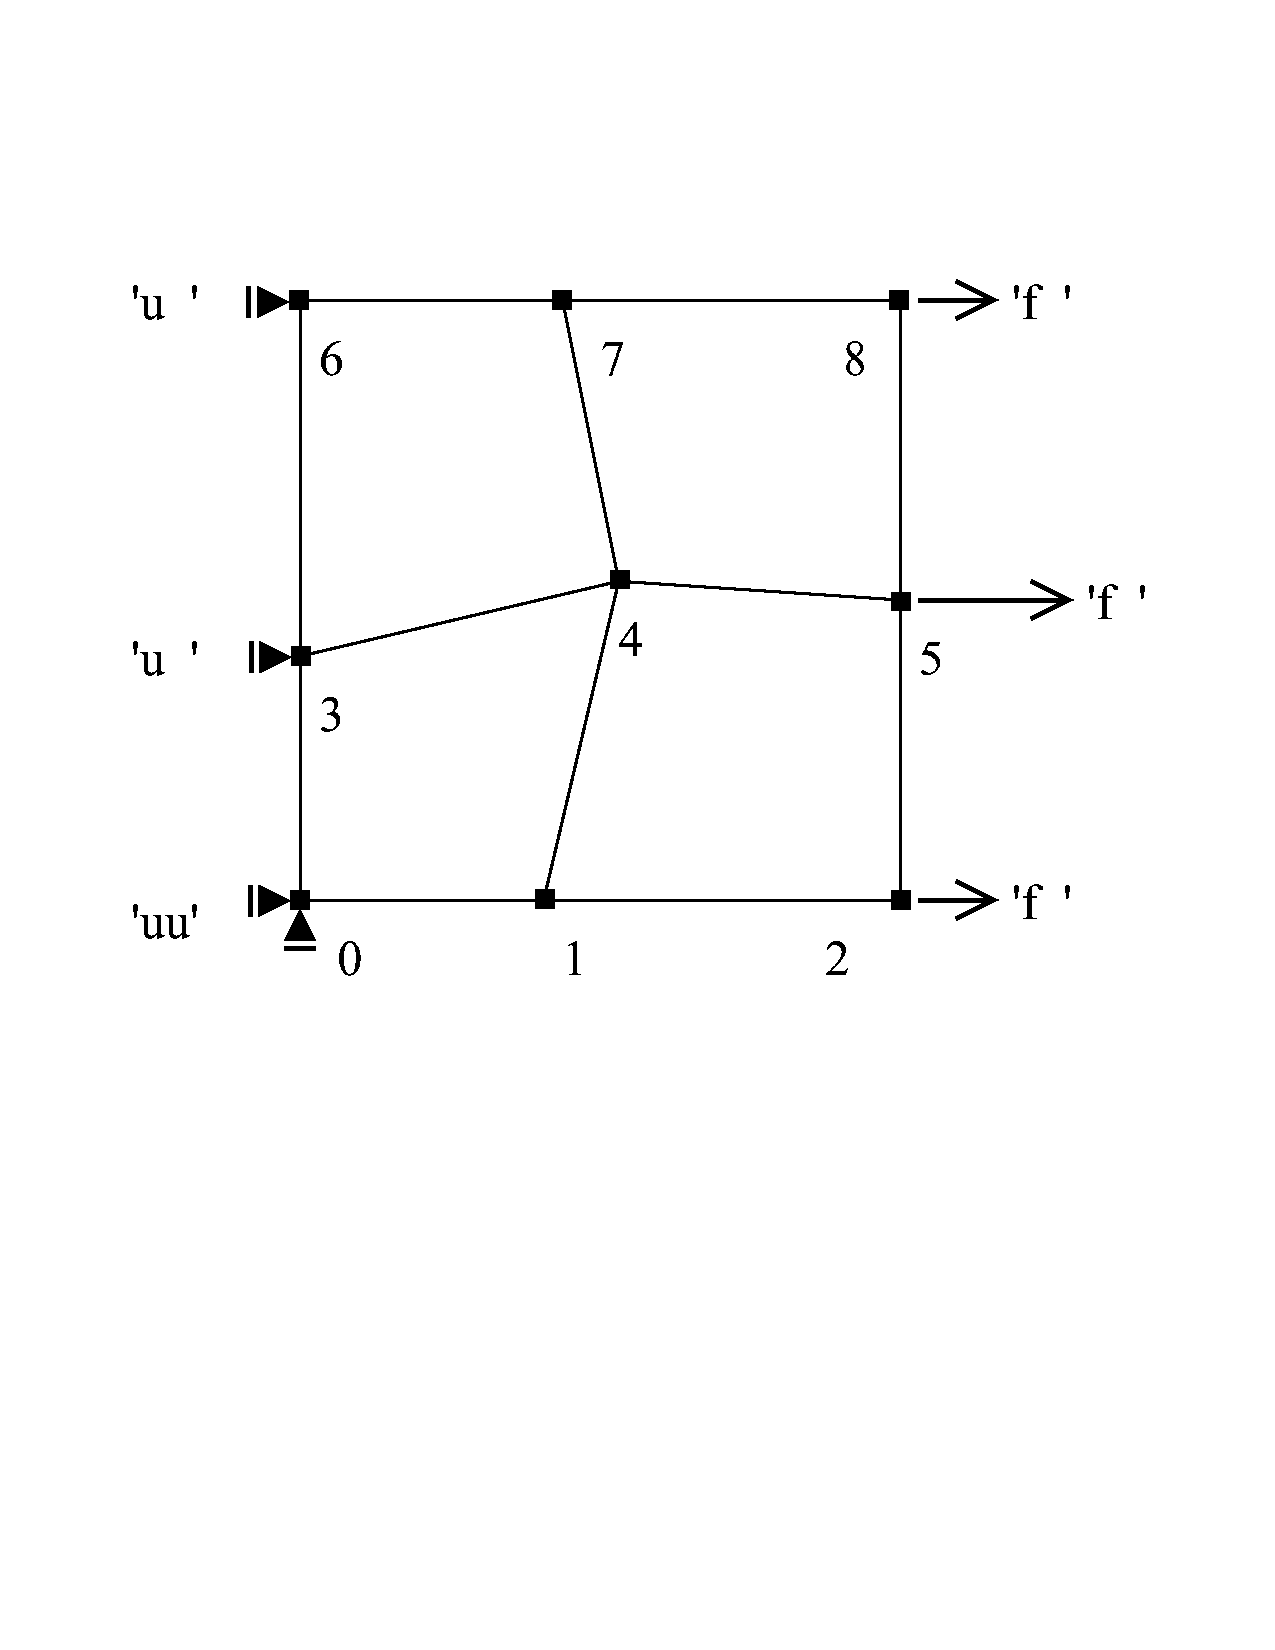
\includegraphics[trim = 0mm 10cm 0mm 1cm, clip, height=8cm]{fig/patchtest.pdf}
  \caption{Patch Test Mesh}
  \label{fig:PatchTestMesh}
\end{figure}

This linear elastic problem is solved under
plane strain assumptions. The material parameters
selected are the following: Youngs's modulus (E)
1000, Poisson ratio (nu) 0.25. The exact solution 
is given as,
\begin{eqnarray}
  u = 0.009375x; ~~ v=-0.003125y \nonumber
\end{eqnarray} 
and stresses are,
\begin{eqnarray}
  \sigma_{xx} = 1.0;~~\sigma_{yy} = 0.0;~~
  \sigma_{xy} = 0.0;~~\sigma_{zz} = 0.25~. \nonumber
\end{eqnarray}

\clearpage
\subsubsection*{Input file (LUA)}
\begin{flushleft}
  \textbf{Inputfile:}
  \ttt{\ttilde/hiqlab/models/tutorial/patch\_test/patch\_test.lua}\\
\end{flushleft}
\hspace{1in}
{\footnotesize
\listinginput[10]{1}{../../../models/tutorial/patch_test/patch_test.lua}
}

\clearpage
\begin{itemize}

  \item{\textbf{Include function definition file:}}
  To use the predefined functions, the definition files
  must be included throught the command \ttt{require}.
  (See section on \ttt{require} command and file \ttt{common.lua}
  for further details).

  \item{\textbf{Construct mesh:}}
  The first line defines and constructs 
  a new \ttt{Mesh} object, where the
  argument "2" defines the physical dimension of
  the mesh ( x,y coordinates). The assignment to 
  {\tt mesh}, passes a reference to the variable.

  \item{\textbf{Construct element:}}
  First a material table \ttt{mtype} is defined. The
  required fields for a static mechanical problem are 
  the Youngs modulus \ttt{E} and Poisson ration \ttt{nu}.
  This material type, along with the string defining the 
  type of analysis is given to the command \ttt{make\_material\_e}
  which produces an elastic material named \ttt{etype}
  \begin{verbatim}
      etype = make_material_e( mtype, 'planestrain');
  \end{verbatim}
  This element is used when elements are added to the \ttt{mesh}.

  \item{\textbf{Define nodal coordinates and element connectivity:}}
  The following two portions of code define arrays of nodal 
  coordinates and element connectivity. The array \ttt{x}
  stores the x and y coordinates of each node consecutively.
  The array \ttt{con} stores the connectivity
  of each element consecutively. In this case, each set of 4 numbers 
  correspond to the connectivity of each 4-noded bilinear 
  quadrilateral element in the mesh. The order of the node 
  numbering for each quadrilateral is defined as fixing the x
  direction first and sweeping across y. For details on this
  see the section on node numbering for elements in the User's
  manual.
  The numbering of the nodes in Lua is zeros based, coinciding
  with that of C++.
  (See section on Mesh Description of the User's manual for details).

  \item{\textbf{Assign nodes and elements to the mesh:}}
  Nodes and elements are assigned to the mesh by the commands
  \ttt{add\_node} and \ttt{add\_element}. The
  array \ttt{x} with 9 nodes and 
  4 bilinear quadrilateral elements of \ttt{etype} with
  connectivity defined n {\tt con} are added to the mesh.

  \item{\textbf{Define and assign boundary conditions:}}
  Boundary conditions in Lua are defined by functions. Depending
  on the physical dimension of the mesh it takes from 1 (x coordinate)
  to 3 (x,y,z coordinate) arguments. The function should output 
  a string defining the boundary condition and numerical values.
  \ttt{u} denotes a fixed boundary condition, \ttt{f} denotes a 
  forced boundary condition, and a blank denotes that no boundary
  condition will be applied. (See Section on Mesh Description of
  User's manual for details. See Section on Helper Lua function for
  mesh for details on mesheq). The mapping between nodal degrees
  of freedom and order of these slots depends on the order in
  which the elements which link the degrees of freedom are 
  added. 

  Once the boundary condition function defined, it is assigned 
  to the mesh through the \ttt{set\_bc} command.

\end{itemize}

\clearpage
\subsubsection*{Solve static problem (MATLAB)}
\begin{flushleft}
  \textbf{Inputfile:}
  \ttt{\ttilde/hiqlab/models/tutorial/patch\_test/patch\_test.m}\\
\end{flushleft}
\hspace{1in}
{\footnotesize
\listinginput[10]{1}{../../../models/tutorial/patch_test/patch_test.m}
}

\clearpage
Once the mesh is defined, the next step is to solve the problem.
This can be done both in Lua and MATLAB. Here we present the MATLAB
interface. 

\begin{itemize}

  \item{\textbf{Load input file}}
  First the Lua mesh input file must be loaded.
  This is conducted by the \ttt{Mesh\_load} command
  which returns a reference to the \ttt{mesh} object 
  and a reference to the variables in the Lua file. 
  One can interact with the Lua input file through 
  this handle \ttt{L}.

  \item{\textbf{View mesh}}
  The mesh can be viewed with the \ttt{plotmesh} command. 
  An optional structure \ttt{opt} can be passed as
  an argument for several options. In this case the
  axis equal feature is activated. 
  The mesh plot for this example
  is shown in Figure \ref{fig:PatchTestMeshMATLAB}. The
  nodes with displacement boundary conditions have a green cross,
  and the nodes with forced boundary conditions have a red cross
  overlayed. 

  \item{\textbf{Solve static problem}}
  The stiffness matrix and forcing vectors are formed and
  and solved for the displacements by the \ttt{static\_state}
  function. The residual of the equilibrium equations is 
  defined as,
  \begin{eqnarray}
  R(u) &=& P(u) - F
  \end{eqnarray}
  where $F$ is the vector of applied forces, $u$
  is the vector of displacments, and for a static
  linear elastic problem $P$ is defined as,
  \begin{eqnarray}
  P   &=& K u~~.
  \end{eqnarray}
  \ttt{static\_state} solves this equation in both the
  linear case and nonlinear case. To invoke the nonlinear 
  case an option must be passed.

  \item{\textbf{Display results}}
  The displacements can be visualized by the command 
  \ttt{plotfield2d}.
  An optional structure \ttt{opt} can be passed as
  an argument for several options. In this case the
  the displacements are magnified 10 times in the 
  visualization.  
  The $x,y$ displacements for this example
  are shown in Figure \ref{fig:PatchTestDisplacements}. The
  top figure shows the $x$ displacements and the bottom shows
  the $y$ displacements. The colors represent the magnitude
  of the displacements, red for positive and blue for negative
  displacements.

\end{itemize}

\begin{figure}[htbp]
  \begin{minipage}{0.45\linewidth}
    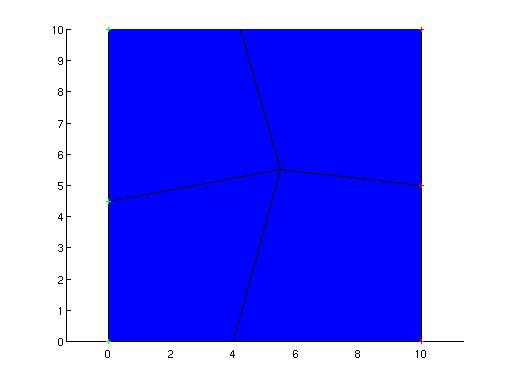
\includegraphics[width=\linewidth]{fig/patch_test_mesh_matlab.jpg}
    \caption{Patch Test Mesh from MATLAB}
    \label{fig:PatchTestMeshMATLAB}
  \end{minipage}
  \hfill
  \begin{minipage}{0.45\linewidth}
    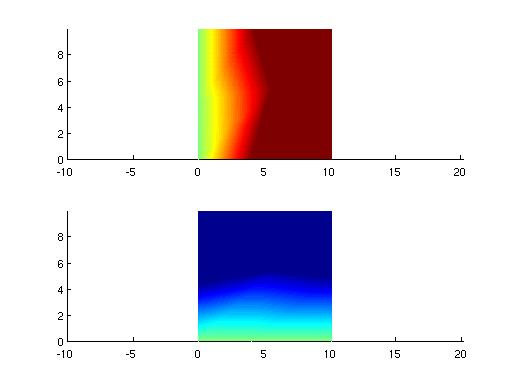
\includegraphics[width=\linewidth]{fig/patch_test_disp_matlab.jpg}
    \caption{Patch Test Displacements}
    \label{fig:PatchTestDisplacements}
  \end{minipage}
\end{figure}

\clearpage
\subsection{2D Cantilever Beam}
\begin{flushleft}
  \textbf{Inputfile:}
  \ttt{\ttilde/hiqlab/models/tutorial/cantilever\_beam}\\
  \textbf{Lua features introduced:}
  \ttt{blocks2d, blocks2dn, mesheq, order, dense}\\
  \textbf{MATLAB features introduced:}
\end{flushleft}
Here we present the analysis of a cantilever beam subjected
to a point load at the end. This example exhibits
the easy to use block commands to define the mesh, as well as 
global parameters that are used for convenience. 

The 10-by-2 2D cantilever beam in Figure \ref{fig:CantileverBeam}, 
which is fixed on the left end and has a unit force applied at the 
right end, is analyzed. 
\begin{figure}[htbp]
  \centering
  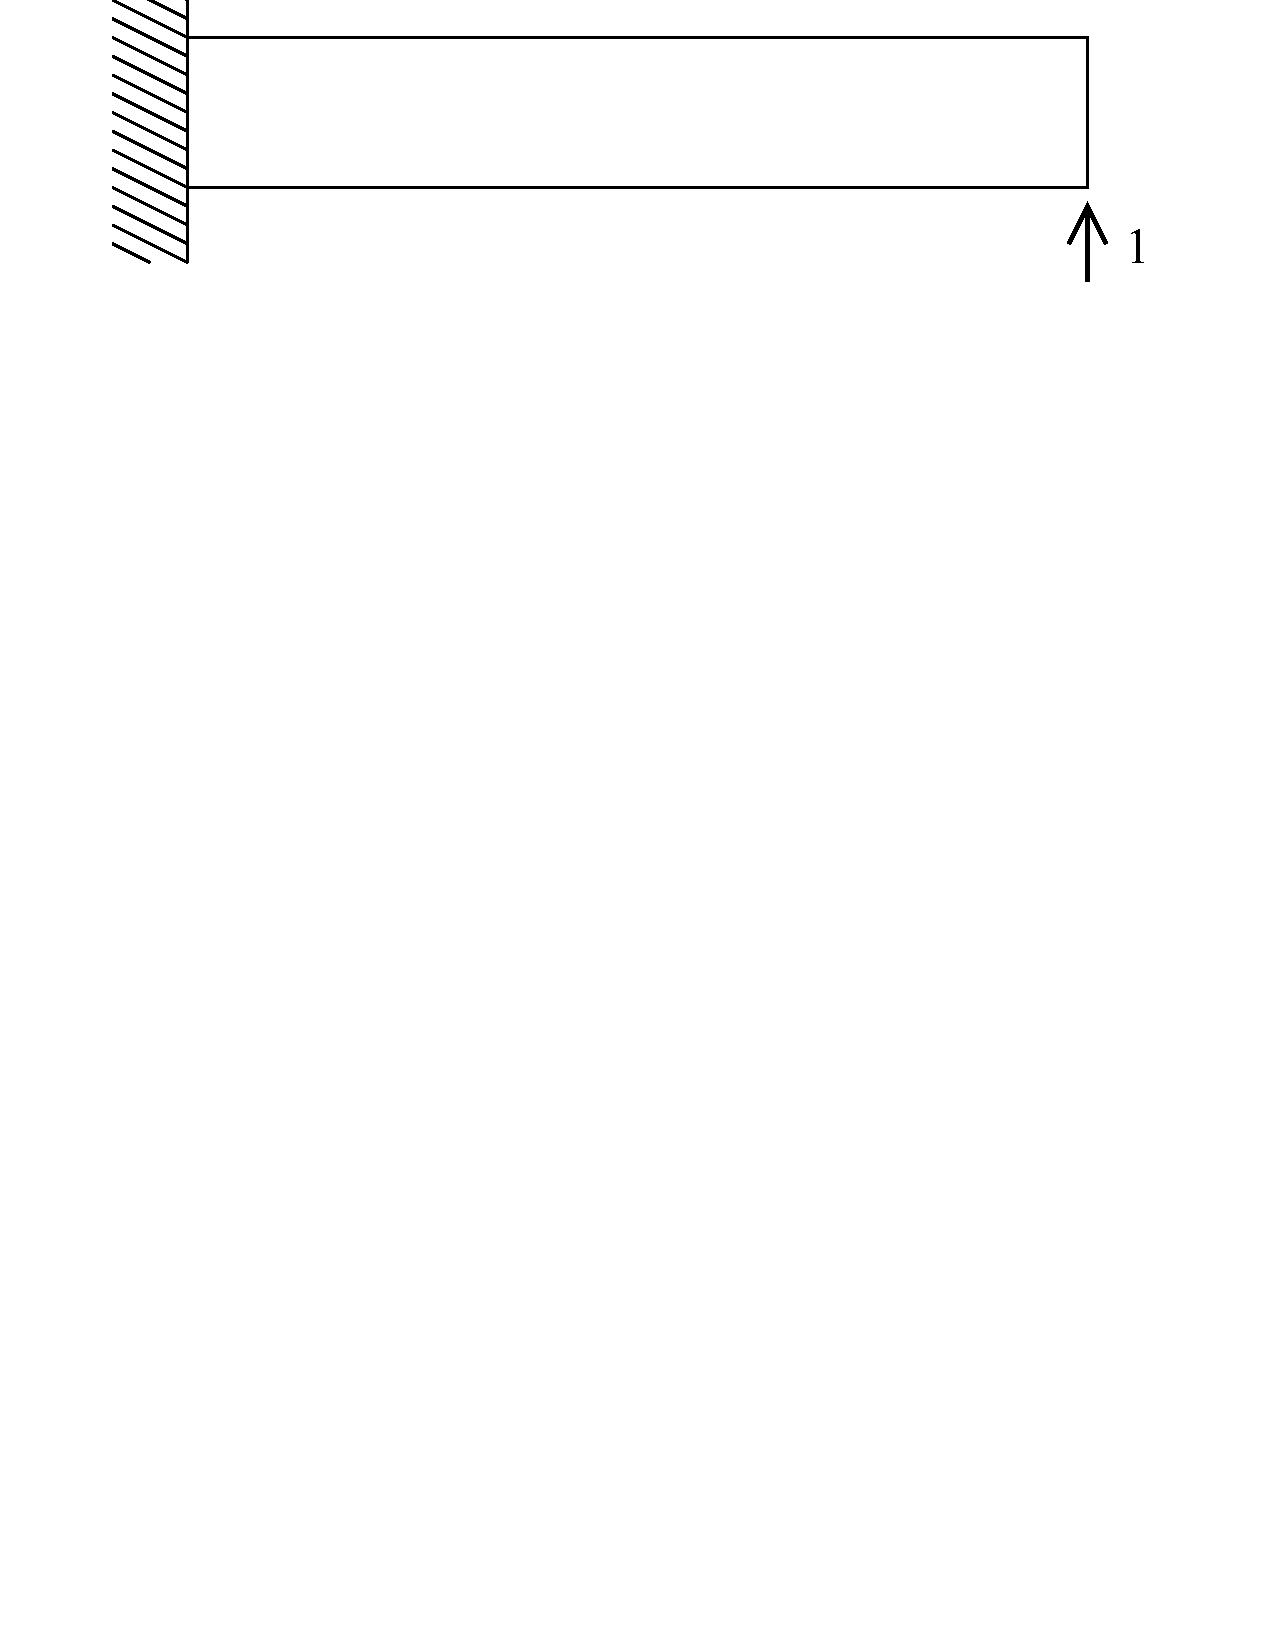
\includegraphics[trim = 0mm 9in 0mm 0cm, clip, height=1in]{fig/cantileverbeam.pdf}
  \caption{Cantilever Beam}
  \label{fig:CantileverBeam}
\end{figure}

Three different Lua mesh input files are presented to solve 
the same problem.
\begin{enumerate}

  \item{\ttt{beam\_test.lua}}: Uses standard \ttt{add\_nodes} and
  \ttt{add\_elements} commands to construct mesh.

  \item{\ttt{beam\_test\_blocks2dn.lua}}: Uses the \ttt{add\_blocks2dn}
  command to construct mesh.

  \item{\ttt{beam\_test\_blocks2d.lua}}: Uses the \ttt{add\_blocks2d}
  command to construct mesh.

\end{enumerate}
The first file is presented to express the tedium involved in
using the \ttt{add\_nodes} and \ttt{add\_elements} command when
the number of nodes and elements increases. This tedium can be 
avoided by using the block generators that are available. The
latter two files use two of these to generate the mesh. All
three files use the same MATLAB file to execute,
\begin{enumerate}
  \item{\ttt{beam\_test.m}}
\end{enumerate}
since only the Lua mesh input file differ. 

\clearpage

\subsubsection*{Input file (LUA)}
\begin{flushleft}
  \textbf{Inputfile:}
  \ttt{\ttilde/hiqlab/models/tutorial/cantilever\_beam/beam\_test.lua}\\
  \ttt{\ttilde/hiqlab/models/tutorial/cantilever\_beam/beam\_test\_blocks2dn.lua}\\
  \ttt{\ttilde/hiqlab/models/tutorial/cantilever\_beam/beam\_test\_blocks2d.lua}\\
\end{flushleft}
\hspace{1in}
\begin{figure}[htbp]
  {\footnotesize
  \listinginput[10]{1}{lua/beam_test_mutual.lua.tex}
  }
  \caption{Matching part of Lua Input file for cantilever beam}
  \label{fig:LuaFile:beam_test_mutual.lua}
\end{figure}

\clearpage
Figure \ref{fig:LuaFile:beam_test_mutual.lua} is the
part of the Lua file that overlap within the three input
files. The portion 'Define nodes and elements' and 
'Add nodes and elements to mesh' differs between the three files. 

\begin{itemize}

  \item{\textbf{Include function definition file:}}
  To use the predefined functions, the definition files
  must be included throught the command \ttt{require}.
  (See section on \ttt{require} command and file \ttt{common.lua}
  for further details).

  \item{\textbf{Construct mesh:}}
  The first line defines and constructs 
  a new \ttt{Mesh} object, where the
  argument "2" defines the physical dimension of
  the mesh ( x,y coordinates). The assignment to 
  \ttt{mesh}, passes a reference to the variable.

  \item{\textbf{Construct element:}}
  First a material table \ttt{mtype} is defined. The
  required fields for a static mechanical problem are 
  the Youngs modulus \ttt{E} and Poisson ration \ttt{nu}.
  This material type, along with the string defining the 
  type of analysis is given to the command \ttt{make\_material\_e}
  which produces an elastic material named \ttt{etype}.
  \begin{verbatim}
      etype = make_material_e( mtype, 'planestrain');
  \end{verbatim}
  This element is used when elements are added to the \ttt{mesh}.

  \item{\textbf{Define nodal coordinates and element connectivity:}}
  \item{\textbf{Assign nodes and elements to the mesh:}}
  This portion of the code differs between the three files.
  Each code generate a beam with 8 quadrilateral bilinear 
  elements, but the amount of code required to define this
  greatly differ. What should be emphasized is the short
  amount of code required when block generators are used.
  (See section on block generators for more details).

  In each case \ttt{div\_x, div\_y} define the number of 
  elements along the $x,y$ direction, \ttt{order} defines the
  order of the elements to be used which is in this case one(linear),
  \ttt{dense\_x,dense\_y} define the approximate size of an 
  element. 
  \begin{enumerate}

    \item{\ttt{beam\_test.lua}}
    Uses standard for loops to define the nodal array \ttt{x} and
    connectivity array \ttt{con}, and then adds these to the 
    mesh through the commands \ttt{add\_node} and \ttt{add\_element}.
    Due to the various indices, this code is error prone. 

    \item{\ttt{beam\_test\_blocks2dn.lua}}
    Uses the \ttt{add\_blocks2d} command to define a block of 
    elements with linear order. The block is defined to have 
    \ttt{div\_x+1=5} nodes along the $x$ direction and 
    \ttt{div\_y+1=3} nodes along the $y$ direction.

    \item{\ttt{beam\_test\_blocks2d.lua}}
    Uses the \ttt{add\_blocks2d} command to define a block of 
    elements with linear order. The block is defined to have 
    \ttt{div\_x+1=5} nodes along the $x$ direction and 
    \ttt{div\_y+1=3} nodes along the $y$ direction.
  \end{enumerate}

  \item{\textbf{Define and assign boundary conditions:}}
  Boundary conditions in Lua are defined by functions. Depending
  on the physical dimension of the mesh it takes from 1 (x coordinate)
  to 3 (x,y,z coordinate) arguments. The function should output 
  a string defining the boundary condition and numerical values.
  \ttt{u} denotes a fixed boundary condition, \ttt{f} denotes a 
  forced boundary condition, and a blank denotes that no boundary
  condition will be applied. (See Section on Mesh Description of
  User's manual for details. See Section on Helper Lua function for
  mesh for details on mesheq).

  Once the boundary condition function defined, it is assigned 
  to the mesh through the \ttt{set\_bc} command.

\end{itemize}


\clearpage
\begin{figure}[htbp]
  {\footnotesize
  \listinginput[10]{1}{lua/beam_test_orig.lua.tex}
  }
  \caption{Differing part of Lua Input file for cantilever 
                                     beam(\ttt{beam\_test.lua})}
  \label{fig:LuaFile:beam_test.lua}
%\end{figure}
%\begin{figure}[htbp]
  {\footnotesize
  \listinginput[10]{1}{lua/beam_test_blocks2dn.lua.tex}
  }
  \caption{Differing part of Lua Input file for cantilever 
                         beam(\ttt{beam\_test\_blocks2dn.lua})}
  \label{fig:LuaFile:beam_test_blocks2dn.lua}
%\end{figure}
%\begin{figure}[htbp]
  {\footnotesize
  \listinginput[10]{1}{lua/beam_test_blocks2d.lua.tex}
  }
  \caption{Differing part of Lua Input file for cantilever 
                         beam(\ttt{beam\_test\_blocks2d.lua})}
  \label{fig:LuaFile:beam_test_blocks2d.lua}
\end{figure}

\clearpage
\subsubsection*{Solve static problem (MATLAB)}
\begin{flushleft}
  \textbf{Inputfile:}
  \ttt{\ttilde/hiqlab/models/tutorial/cantilever\_beam/beam\_test.m}\\
\end{flushleft}
\hspace{1in}
{\footnotesize
\listinginput[10]{1}{../../../models/tutorial/cantilever_beam/beam_test.m}
}
Once the mesh is defined, the next step is to solve the problem.
This can be done both in Lua and MATLAB. Here we present the MATLAB
interface. This file is identical
to the patch\_test and we refer to the section for details.
The mesh and displacements are shown in 
Figure \ref{fig:CantileverBeamMeshMATLAB}
and Figure \ref{fig:CantileverBeamDisplacements}.

\begin{figure}[htbp]
  \begin{minipage}{0.45\linewidth}
    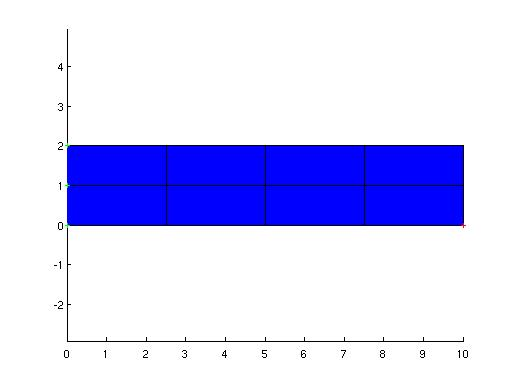
\includegraphics[width=\linewidth]{fig/cantilever_beam_mesh_matlab.jpg}
    \caption{Cantilever Beam mesh from MATLAB}
    \label{fig:CantileverBeamMeshMATLAB}
  \end{minipage}
  \hfill
  \begin{minipage}{0.45\linewidth}
    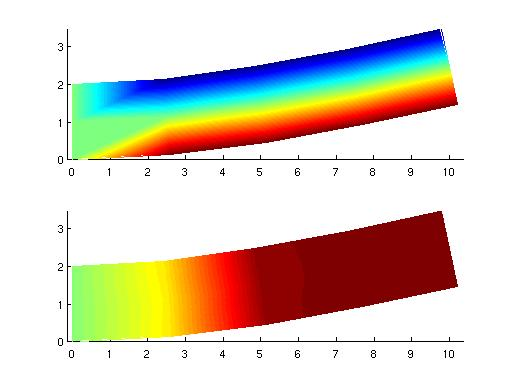
\includegraphics[width=\linewidth]{fig/cantilever_beam_disp_matlab.jpg}
    \caption{Cantilever Beam Displacements}
    \label{fig:CantileverBeamDisplacements}
  \end{minipage}
\end{figure}

\clearpage
\subsection{Circular Disk}
\begin{flushleft}
  \textbf{Inputfile:}
  \ttt{\ttilde/hiqlab/models/tutorial/circular\_disk}\\
  \textbf{Lua features introduced:}
  \ttt{add\_block\_shape, add\_curved\_block\_shape2d, tie, meshtol, or}
  \textbf{MATLAB features introduced:}
  Using params in \ttt{Mesh\_load}
\end{flushleft}
Here we present the analysis of a circular disk subjected
to a point load at the top and bottom. This example exhibits
the easy to use block commands to define the curved meshes,
the ability to pass values into the Lua mesh input file, and 
global parameters that are used for convenience. 

The unit circular disk in Figure \ref{fig:CircularDisk}, which
is 4-fold symmetric is analyzed. Due to this symmetry, only
the quarter in Figure \ref{fig:CircularDiskQuarter} is meshed.
The $y$ displacements of the bottom edge is set to zero, as well as
the $x$ displacements of the left edge. A force of -5 is applied
at the top most node in the $x$ direction. 

In this example, block generators are used  to mesh this disk.
The disk is divided into the 3 parts with corresponding control
nodes shown in Figure \ref{fig:CircularDiskQuarter}.

\begin{figure}[htbp]
  \begin{minipage}{0.45\linewidth}
    \centering
    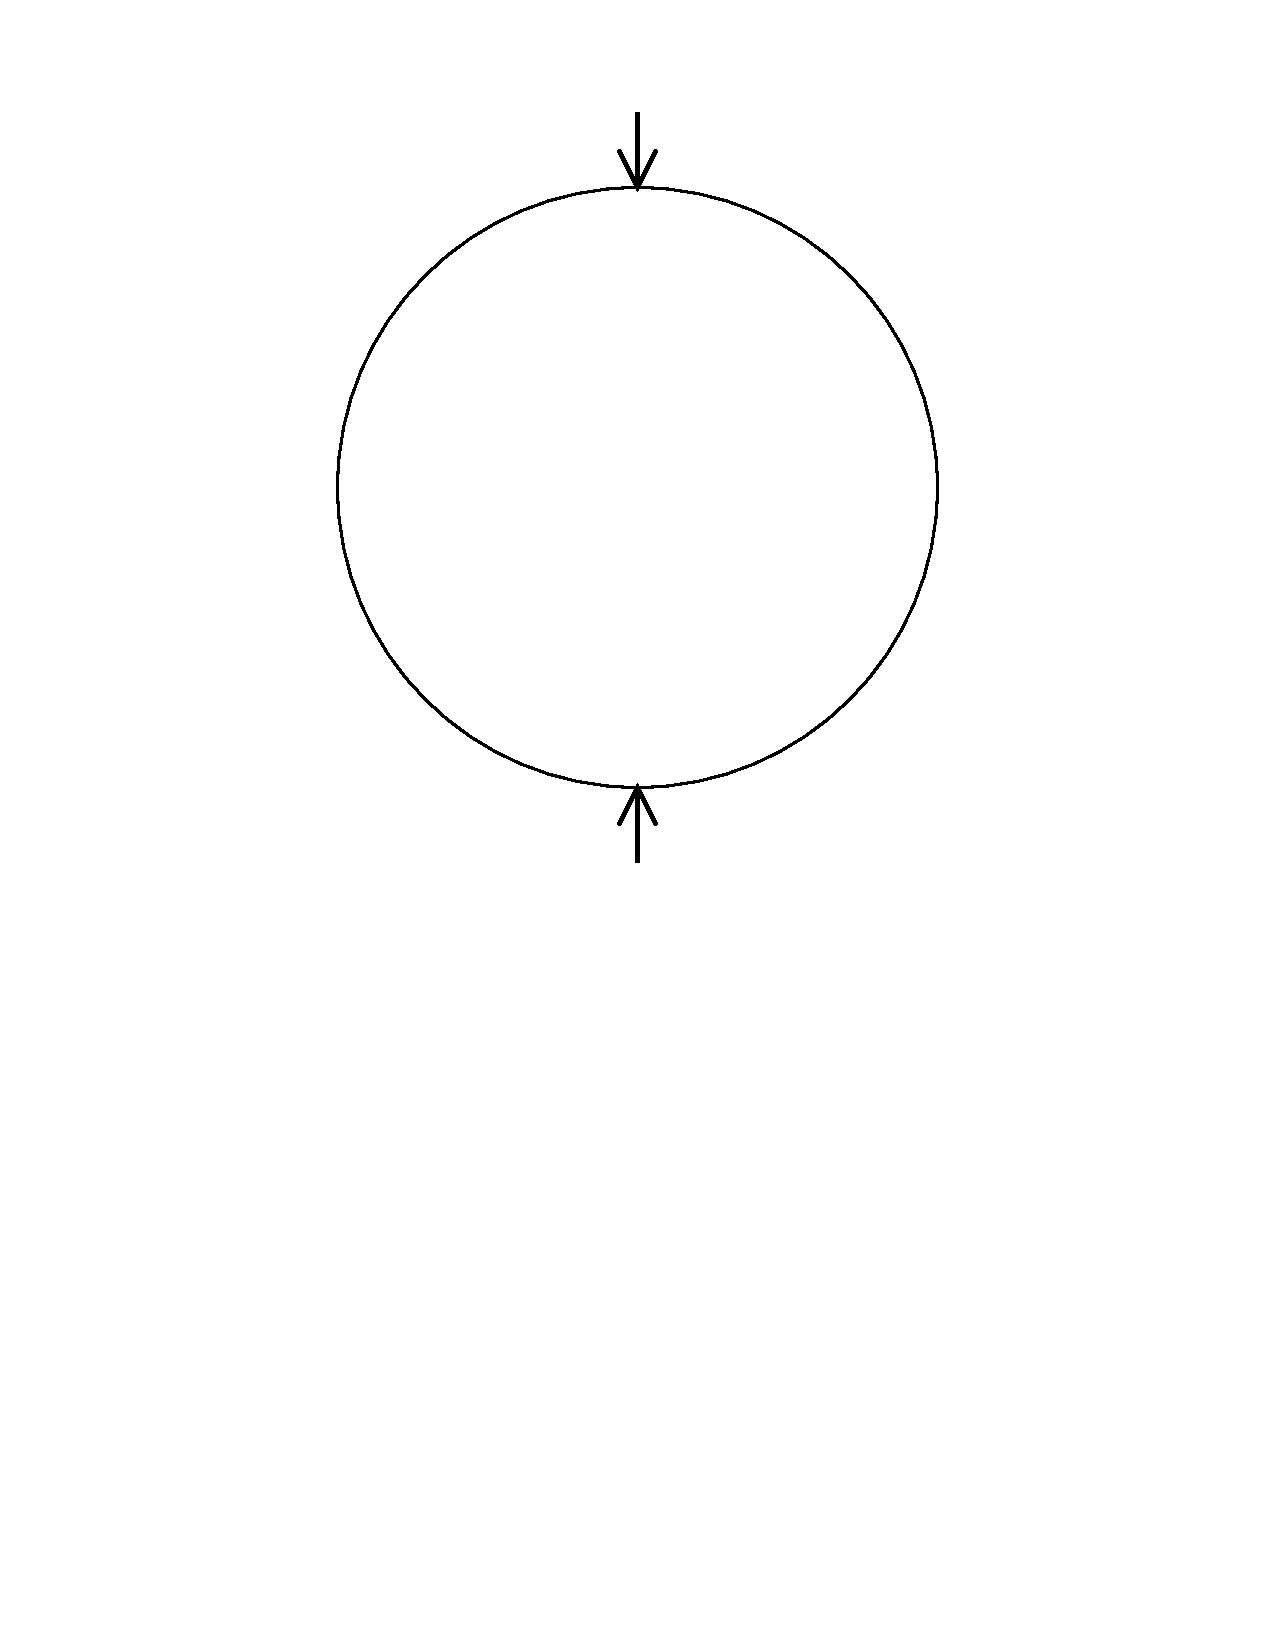
\includegraphics[trim = 1in 5in 1in 0cm, clip, height=2in]{fig/circulardisk.pdf}
    \caption{Circular Disk}
    \label{fig:CircularDisk}
  \end{minipage}
  \begin{minipage}{0.45\linewidth}
    \centering
    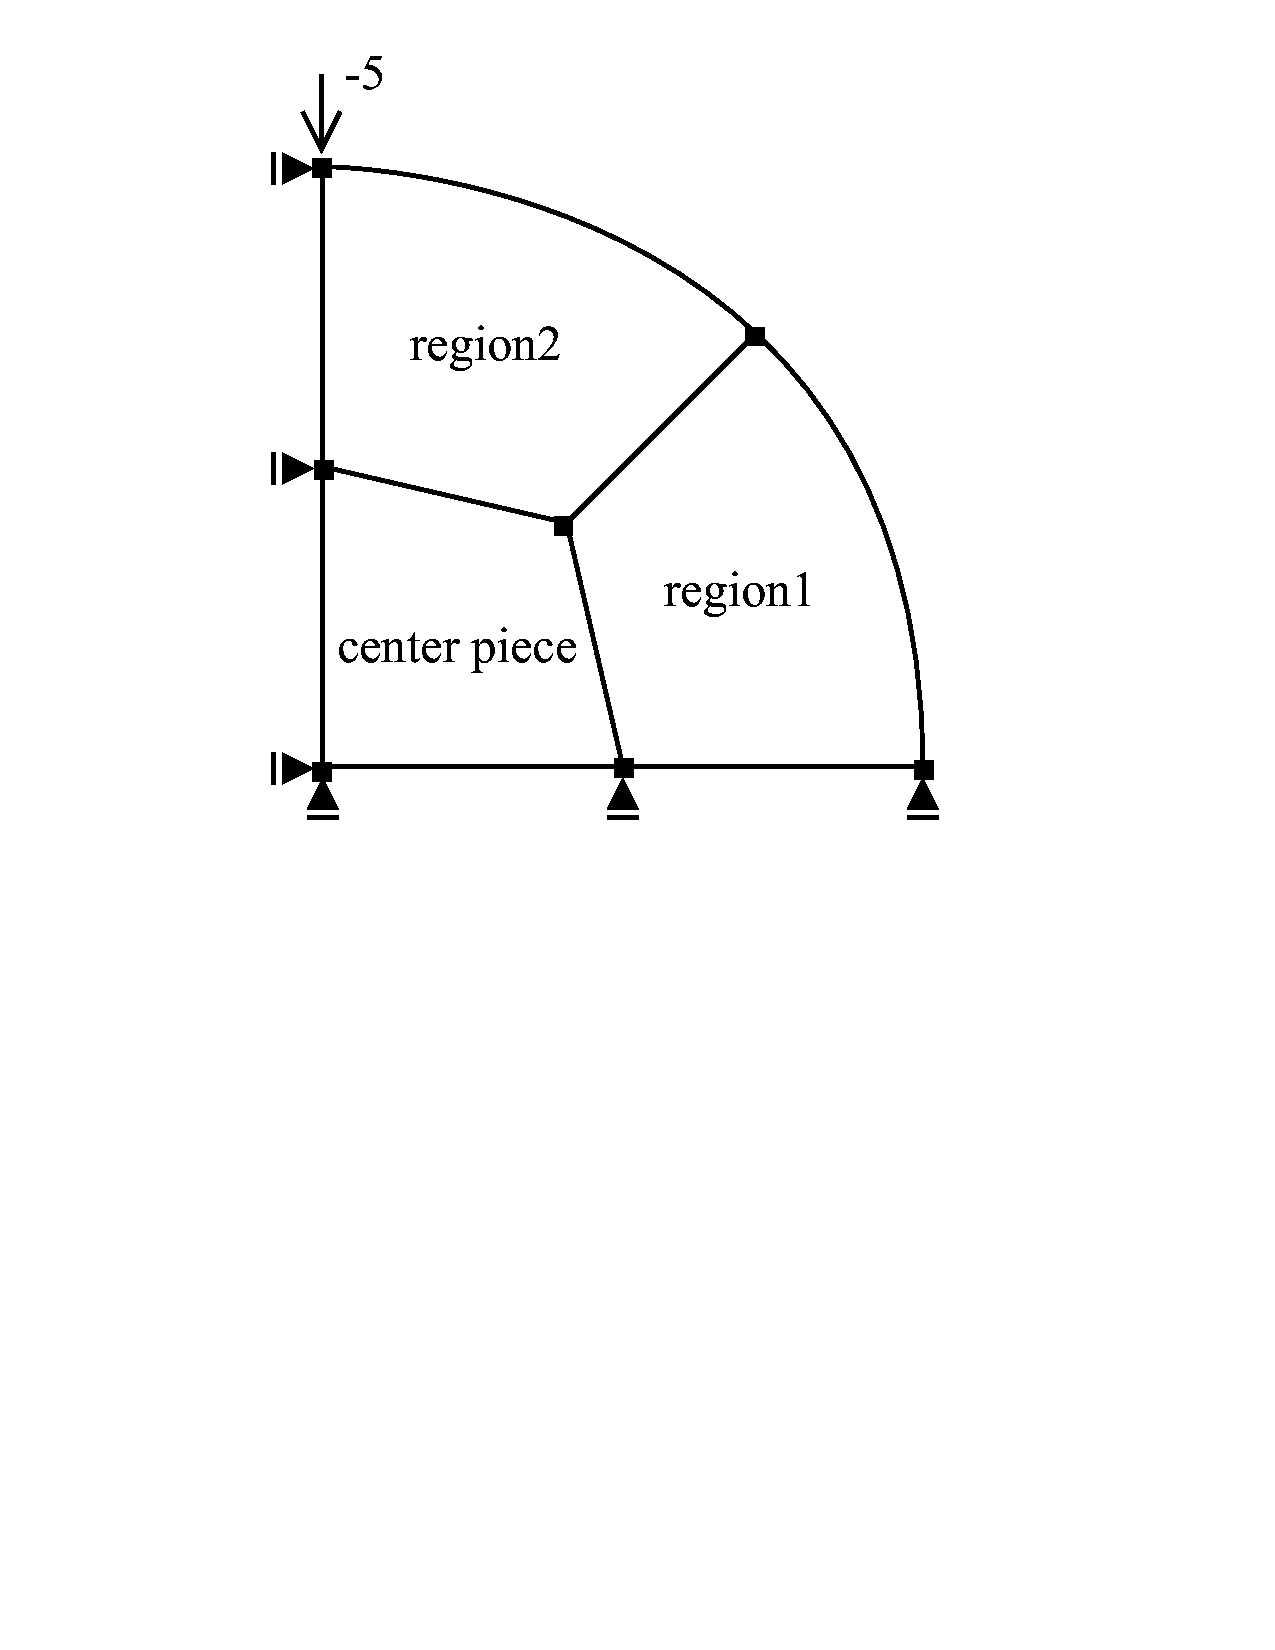
\includegraphics[trim = 0.5in 5in 0.5in 0cm, clip, height=2in]{fig/circulardiskquarter.pdf}
    \caption{Quarter of the Circular Disk}
    \label{fig:CircularDiskQuarter}
  \end{minipage}
\end{figure}

\clearpage
\subsubsection*{Input file (LUA)}
\begin{flushleft}
  \textbf{Inputfile:}
  \ttt{\ttilde/hiqlab/models/tutorial/circular\_disk/circular\_disk.lua}\\
\end{flushleft}
\hspace{1in}
{\footnotesize
\listinginput[10]{1}{../../../models/tutorial/circular_disk/circular_disk.lua}
}

\clearpage
\begin{itemize}

  \item{\textbf{Include function definition file:}}
  To use the predefined functions, the definition files
  must be included throught the command \ttt{require}.
  (See section on \ttt{require} command and file \ttt{common.lua}
  for further details).

  \item{\textbf{Construct mesh:}}
  The first line defines and constructs 
  a new \ttt{Mesh} object, where the
  argument "2" defines the physical dimension of
  the mesh ( x,y coordinates). The assignment to 
  \ttt{mesh}, passes a reference to the variable.

  \item{\textbf{Construct element:}}
  First a material table \ttt{mtype} is defined. The
  required fields for a static mechanical problem are 
  the Youngs modulus \ttt{E} and Poisson ration \ttt{nu}.
  This material type, along with the string defining the 
  type of analysis is given to the command \ttt{make\_material\_e}
  which produces an elastic material.
  \begin{verbatim}
      etype = make_material_e( mtype, 'planestrain');
  \end{verbatim}
  named \ttt{etype}.
  This element is used when elements are added to the \ttt{mesh}.

  \item{\textbf{Define number of elements along the blocks and element order:}}
  \ttt{num\_elem} defines the number of elements that are placed along
  the $x,y$ directions of the 3 blocks, center piece, region1 and region2.
  \ttt{order} defines the order of each of these elements. By defining
  these variables with the \ttt{or} statement, it allows one to pass
  parameters from the running MATLAB environment into the Lua environment.
  If the variables \ttt{num\_elem,order} are not predefined, they are 
  set to 1 respectively. \ttt{div\_x,div\_y} define how many nodes the 
  blocks have along each edge. 

  \item{\textbf{Define mesh tolerance:}}
  When the variable \ttt{meshtol} is defined, functions such as 
  \ttt{tie, mesheq, meshle, meshge, meshbetween} take this as a default
  value when no argument considering tolerance is given. This can be 
  observed in the boundary function definition.

  \item{\textbf{Define nodal coordinates:}}
  The control nodes for the blocks are defined. \ttt{xc} defines the 
  control nodes for the center piece, \ttt{xr1} for region1, and 
  \ttt{xr2} for region2. Since region1 and region2 are curved blocks,
  curved block generators are applied. This function requires that
  the curvature on the 4 edges be defined. These values are stored in
  \ttt{curv1} and \ttt{curv2} respectively. (see section on block
  generators for details).

  \item{\textbf{Define mesh using block command:}}
  \ttt{add\_block\_shape} is used to isoparametrically map a square
  block to mesh the center piece. Region1 and region2 are meshed by
  the \ttt{add\_curved\_block\_shape2d}.

  \item{\textbf{Tie the mesh together:}}
  The three blocks, center piece, region1, and region2 are tied
  together by the \ttt{tie} command. This function ties together 
  nodes that are within a determined tolerance. Since \ttt{meshtol} 
  is predefined, no argument is required.(See section on mesh
  description for details).

  \item{\textbf{Define and assign boundary conditions:}}  
  Boundary conditions in Lua are defined by functions. Depending
  on the physical dimension of the mesh it takes from 1 (x coordinate)
  to 3 (x,y,z coordinate) arguments. The boundary condition for
  this problem requires that the node at (0,1) have fixed $x$ displacement
  of zero and force of $-5$ in the $y$ direction. The first \ttt{return}
  argument corresponds to this condition. The second \ttt{return} argument
  defines the zero $x$ displacement boundary condition for the left edge,
  and the third the zero $y$ displacement boundary condition for the 
  bottom edge. (See Section on Mesh Description of
  User's manual for details. See Section on Helper Lua function for
  mesh for details on mesheq).

  Once the boundary condition function defined, it is assigned 
  to the mesh through the \ttt{set\_bc} command.

\end{itemize}

\clearpage
\subsubsection*{Solve static problem (MATLAB)}
\begin{flushleft}
  \textbf{Inputfile:}
  \ttt{\ttilde/hiqlab/models/tutorial/circular\_disk/circular\_disk.m}\\
\end{flushleft}
\hspace{1in}
{\footnotesize
\listinginput[10]{1}{../../../models/tutorial/circular_disk/circular_disk.m}
}

\clearpage
Once the mesh is defined, the next step is to solve the problem.
This can be done both in Lua and MATLAB. Here we present the MATLAB
interface. 

\begin{itemize}

  \item{\textbf{Pass parameters into Lua file}}
  Variables from Matlab can be passed into the Lua input file
  by the optional \ttt{params} structure. For this problem, the
  variables \ttt{num\_elem} and \ttt{order} are passed. In the
  Lua input file, the \ttt{or} argument makes this possible. 
  By constructing the Lua input file in this manner, parameteric
  studies such as mesh refinement are easily conducted. For this
  problem, the two parameters are varied to show this. 

  \item{\textbf{Load input file}}
  The optional structure \ttt{params} is given as an argument,
  to the function \ttt{Mesh\_load}
  to pass variables into the Lua input file environment.

\end{itemize}

\clearpage
\subsubsection*{Parametric study (MATLAB)}
Parametric study conducted by varying the variable 
\ttt{num\_elem} and \ttt{order} in the structure \ttt{params}
passed into the Lua environment is presented in this
section. The mesh and displacement plot obtained for each case
is shown in the figures.

\begin{figure}[htbp]
  \begin{minipage}{0.45\linewidth}
    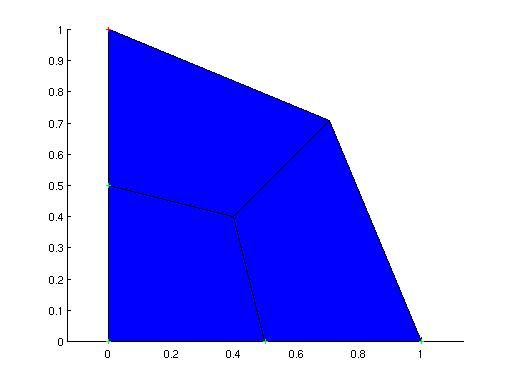
\includegraphics[width=\linewidth]{fig/circular_disk11_mesh_matlab.jpg}
    \caption{Circular Disk mesh from MATLAB(\ttt{num\_elem=1,order=1})}
    \label{fig:CircularDisk11MeshMATLAB}
  \end{minipage}
  \hfill
  \begin{minipage}{0.45\linewidth}
    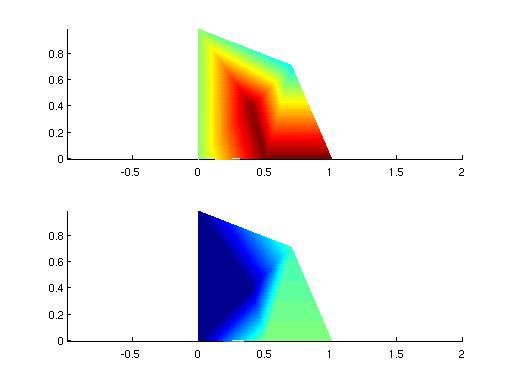
\includegraphics[width=\linewidth]{fig/circular_disk11_disp_matlab.jpg}
    \caption{Circular Disk Displacements(\ttt{num\_elem=1,order=1})}
    \label{fig:CircularDisk11Displacements}
  \end{minipage}
  \begin{minipage}{0.45\linewidth}
    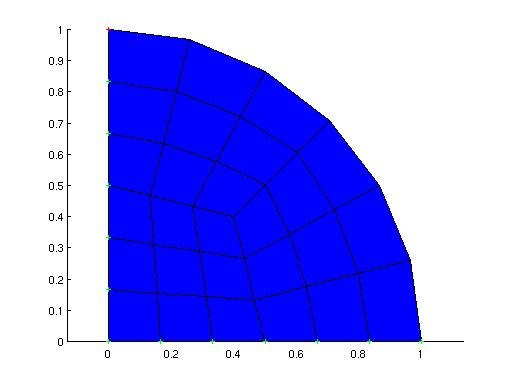
\includegraphics[width=\linewidth]{fig/circular_disk13_mesh_matlab.jpg}
    \caption{Circular Disk mesh from MATLAB(\ttt{num\_elem=1,order=3})}
    \label{fig:CircularDisk13MeshMATLAB}
  \end{minipage}
  \hfill
  \begin{minipage}{0.45\linewidth}
    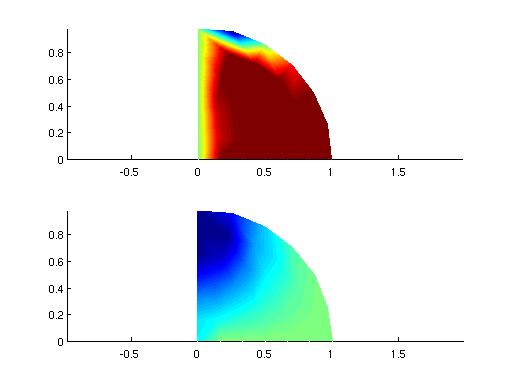
\includegraphics[width=\linewidth]{fig/circular_disk13_disp_matlab.jpg}
    \caption{Circular Disk Displacements(\ttt{num\_elem=1,order=3})}
    \label{fig:CircularDisk13Displacements}
  \end{minipage}
  \begin{minipage}{0.45\linewidth}
    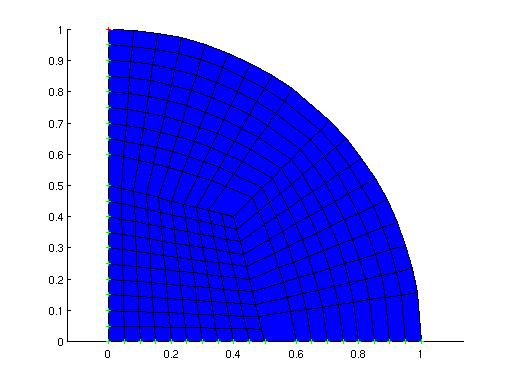
\includegraphics[width=\linewidth]{fig/circular_disk52_mesh_matlab.jpg}
    \caption{Circular Disk mesh from MATLAB(\ttt{num\_elem=5,order=2})}
    \label{fig:CircularDisk52MeshMATLAB}
  \end{minipage}
  \hfill
  \begin{minipage}{0.45\linewidth}
    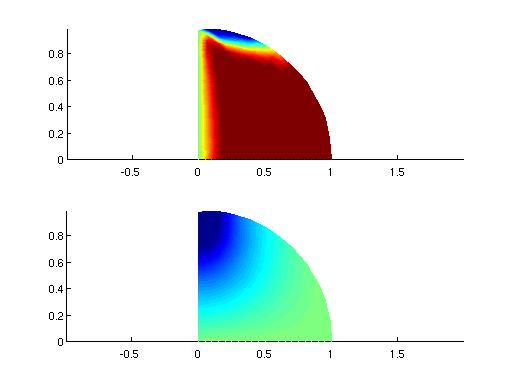
\includegraphics[width=\linewidth]{fig/circular_disk52_disp_matlab.jpg}
    \caption{Circular Disk Displacements(\ttt{num\_elem=5,order=2})}
    \label{fig:CircularDisk52Displacements}
  \end{minipage}
\end{figure}

\clearpage
\subsection{Arch}
\begin{flushleft}
  \textbf{Inputfile:}
  \ttt{\ttilde/hiqlab/models/tutorial/arch}\\
  \textbf{Lua features introduced:}
  \ttt{add\_block\_transform}\\
  \textbf{MATLAB features introduced:}
\end{flushleft}
Here we present the analysis of an arch subjected
to a point load at the top. This example exhibits
the easy to use block commands to define the curved meshes,
the ability to pass values into the Lua mesh input file, and 
global parameters that are used for convenience. 

The arch in Figure \ref{fig:Arch} is analyzed. 
The $x,y$ displacements at the bottom edge is set to zero, and
a force of -5 is applied at the top most node in the $y$ direction. 

In this example, a block generators is used  to mesh this arch.
The control nodes are shown as black squares in  Figure 
\ref{fig:Arch}.

\begin{figure}[htbp]
  \centering
  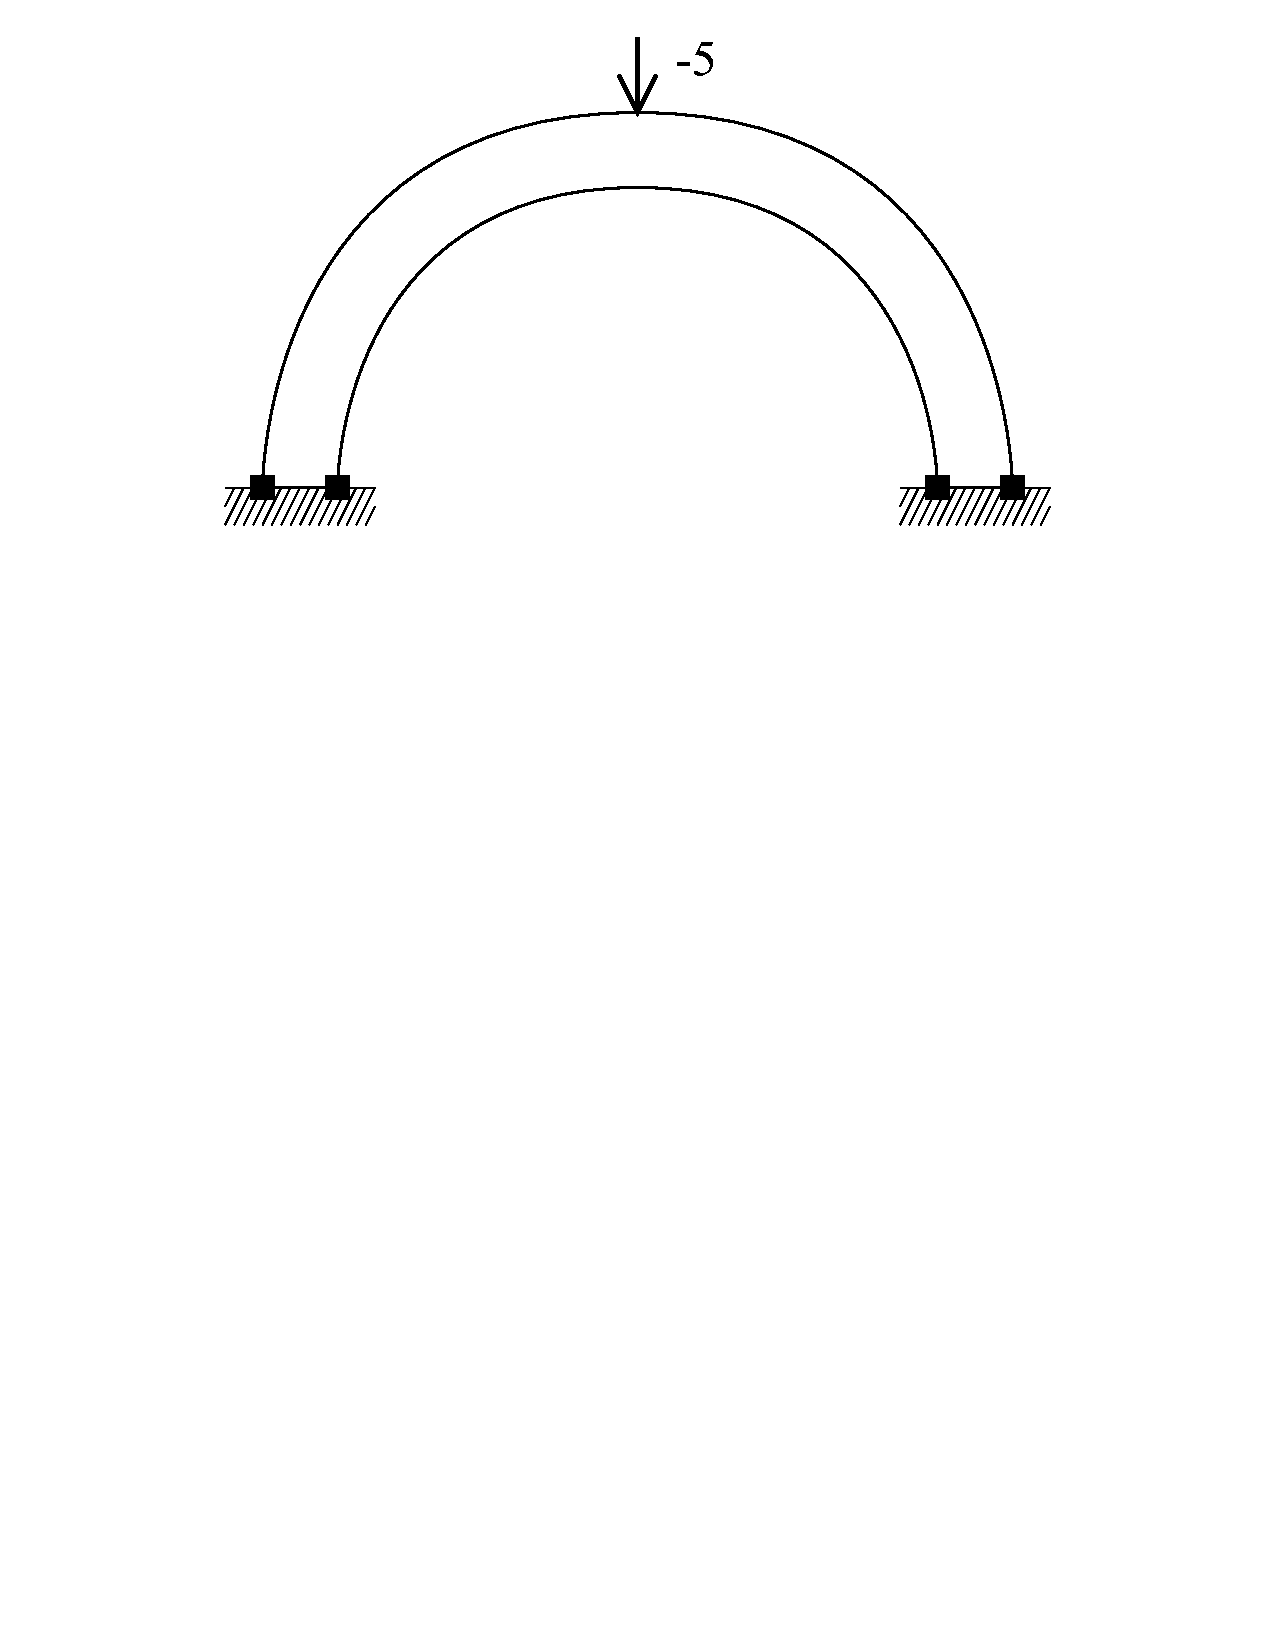
\includegraphics[trim = 1in 5.5in 1in 0cm, clip, height=2in]{fig/arch.pdf}
  \caption{Arch}
  \label{fig:Arch}
\end{figure}

\clearpage
\subsubsection*{Input file (LUA)}
\begin{flushleft}
  \textbf{Inputfile:}
  \ttt{\ttilde/hiqlab/models/tutorial/arch/arch.lua}\\
\end{flushleft}
\hspace{1in}
{\footnotesize
\listinginput[10]{1}{../../../models/tutorial/arch/arch.lua}
}

\clearpage
\begin{itemize}

  \item{\textbf{Define number of elements along the blocks and element order:}}
  \ttt{num\_elem} defines the number of elements that are placed along
  the $y$ directions of the block. The number elements that are placed
  along the $x$ is defined as \ttt{6 num\_elem}.
  \ttt{order} defines the order of each of these elements. By defining
  these variables with the \ttt{or} statement, it allows one to pass
  parameters from the running MATLAB environment into the Lua environment.
  If the variables \ttt{num\_elem,order} are not predefined, they are 
  set to 1 respectively. \ttt{div\_x,div\_y} define how many nodes the 
  blocks have along each edge. 

  \item{\textbf{Define size of arch:}}
  The inner radius of the arch is defined as \ttt{Ri} and the thickness
  by \ttt{Rt}.

  \item{\textbf{Define ring function for block transform:}}
  The function \ttt{ring} which maps a square block to an arch by
  polar coordinate transformation is defined. This function must take
  the $x,y$ coordinates and return new $x,y$ coordinates.

  \item{\textbf{Define mesh using block command:}}
  \ttt{add\_block\_transfor} is used to map a square
  block to an arch by means of polar coordinate transformation.

  \item{\textbf{Define and assign boundary conditions:}}  
  Boundary conditions in Lua are defined by functions. Depending
  on the physical dimension of the mesh it takes from 1 (x coordinate)
  to 3 (x,y,z coordinate) arguments. The boundary condition for
  this problem requires that along the bottom edge the $x,y$ displacements
  are fixed and a force of $-5$ in the $y$ direction at the top node.
  The first \ttt{return} argument corresponds to this condition. 
  The second \ttt{return} argument
  defines the zero $x,y$ displacement boundary condition along the 
  bottom edge.
  (See Section on Mesh Description of
  User's manual for details. See Section on Helper Lua function for
  mesh for details on mesheq).

  Once the boundary condition function defined, it is assigned 
  to the mesh through the \ttt{set\_bc} command.

\end{itemize}

\clearpage
\subsubsection*{Solve static problem (MATLAB)}
\begin{flushleft}
  \textbf{Inputfile:}
  \ttt{\ttilde/hiqlab/models/tutorial/arch/arch.m}\\
\end{flushleft}
\hspace{1in}
{\footnotesize
\listinginput[10]{1}{../../../models/tutorial/arch/arch.m}
}

\clearpage
Once the mesh is defined, the next step is to solve the problem.
This can be done both in Lua and MATLAB. Here we present the MATLAB
interface. 
The mesh and displacement plot obtained for \ttt{node\_num=3,order=2}
is shown in the Figures \ref{fig:Arch32MeshMATLAB} and 
\ref{fig:Arch32Displacements}.

\begin{figure}[htbp]
  \begin{minipage}{0.45\linewidth}
    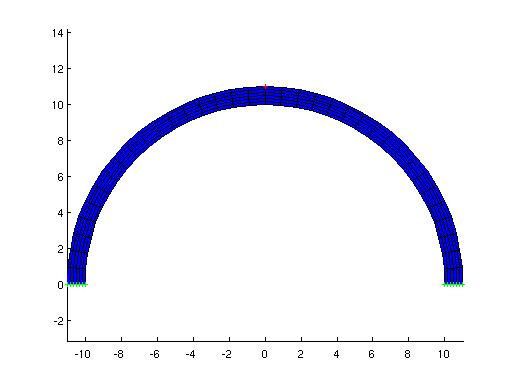
\includegraphics[width=\linewidth]{fig/arch32_mesh_matlab.jpg}
    \caption{Arch mesh from MATLAB (\ttt{num\_elem=3,order=2})}
    \label{fig:Arch32MeshMATLAB}
  \end{minipage}
  \hfill
  \begin{minipage}{0.45\linewidth}
    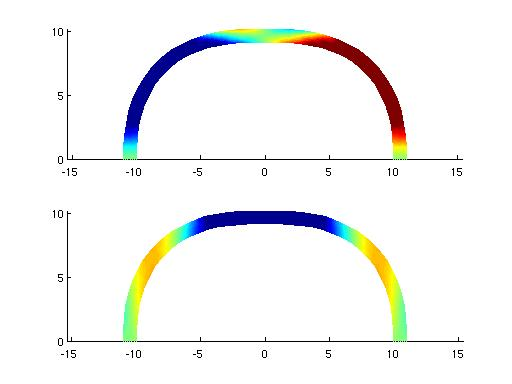
\includegraphics[width=\linewidth]{fig/arch32_disp_matlab.jpg}
    \caption{Arch32 Displacements  (\ttt{num\_elem=3,order=2})}
    \label{fig:Arch32Displacements}
  \end{minipage}
\end{figure}

\clearpage
\section{Anchor loss analysis}
\subsection{1D waves}
\begin{flushleft}
  \textbf{Inputfile:}
  \ttt{\ttilde/hiqlab/models/tutorial/pml1d}\\
  \textbf{Lua features introduced:}
  \ttt{make\_material\_s, add\_block, set\_stretch, f0}\\
  \textbf{MATLAB features introduced:}
  \ttt{Mesh\_assemble\_R, harmonic\_state, plotfield1d, plotcycle1d},
  plotting the stretch function
\end{flushleft}
This example illustrates basic anchor loss
modeling using Perfect Matched Layers. Though
this problem is 1 dimensional, the idea extends
to the multidimensional case. 

Ideally we would like to simulate the situation
shown in part A of Figure \ref{fig:PropagatingWaves},
where a wave propagates into an infinite domain,
resulting in only outgoing waves. Computationally
we cannot model and infinite domain and must truncate
it at a finite length. Blindly applying a fixed boundary
condition at the end results in part B of Figure
\ref{fig:PropagatingWaves}, where we obtain unphysical
standing waves. By applying this method of PML on a 
layer close to the boundary as is shown in light gray in 
Figure \ref{fig:PropagatingWaves}, we are able to regain
the situation in A, where we again have propagating waves.
Waves propagating through the PML layer are exponentially
damped. If the PML layer and a parameter \ttt{f0} that
we mention later are chosen properly, the waves are fully
damped by the time they reach the boundary and produce 
close to zero wave reflections. 

To define this PML we assign the \ttt{stretch\_function} 
mentioned in section ?? to the elements that the PML 
region is defined. The form of the \ttt{stretch\_function}
that is applied for this 1D case is shown in 
Figure \ref{fig:1DPMLSchematic}. The actual equation is,
\begin{eqnarray}
\text{stretch\_function(x)}
&=& \text{max}\left(0, \text{f0} \frac{\text{x-xpml}}
                                      {\text{xrad-xpml}}\right)
\end{eqnarray}
which is a linear function that takes 0 at the initiation of
the PML and \ttt{f0} at the boundary. The performance of the 
PML depends on the length of the PML and parameter \ttt{f0} and
they can be selected heuristically as shown in paper ???. 
In general a long PML and large \ttt{f0} desired, though
increasing the length will increase computational costs and 
as will be seen in the example, increasing the \ttt{f0} without
increasing the mesh density of the elements degrades performance.
In MEMS applications a value of approximately 40 is observed to
give standard performance.
There exists a function in MATLAB named \ttt{estimate\_pml} which
does this. (See section on ????).

\begin{figure}[htbp]
  \begin{minipage}{0.45\linewidth}
  \centering
  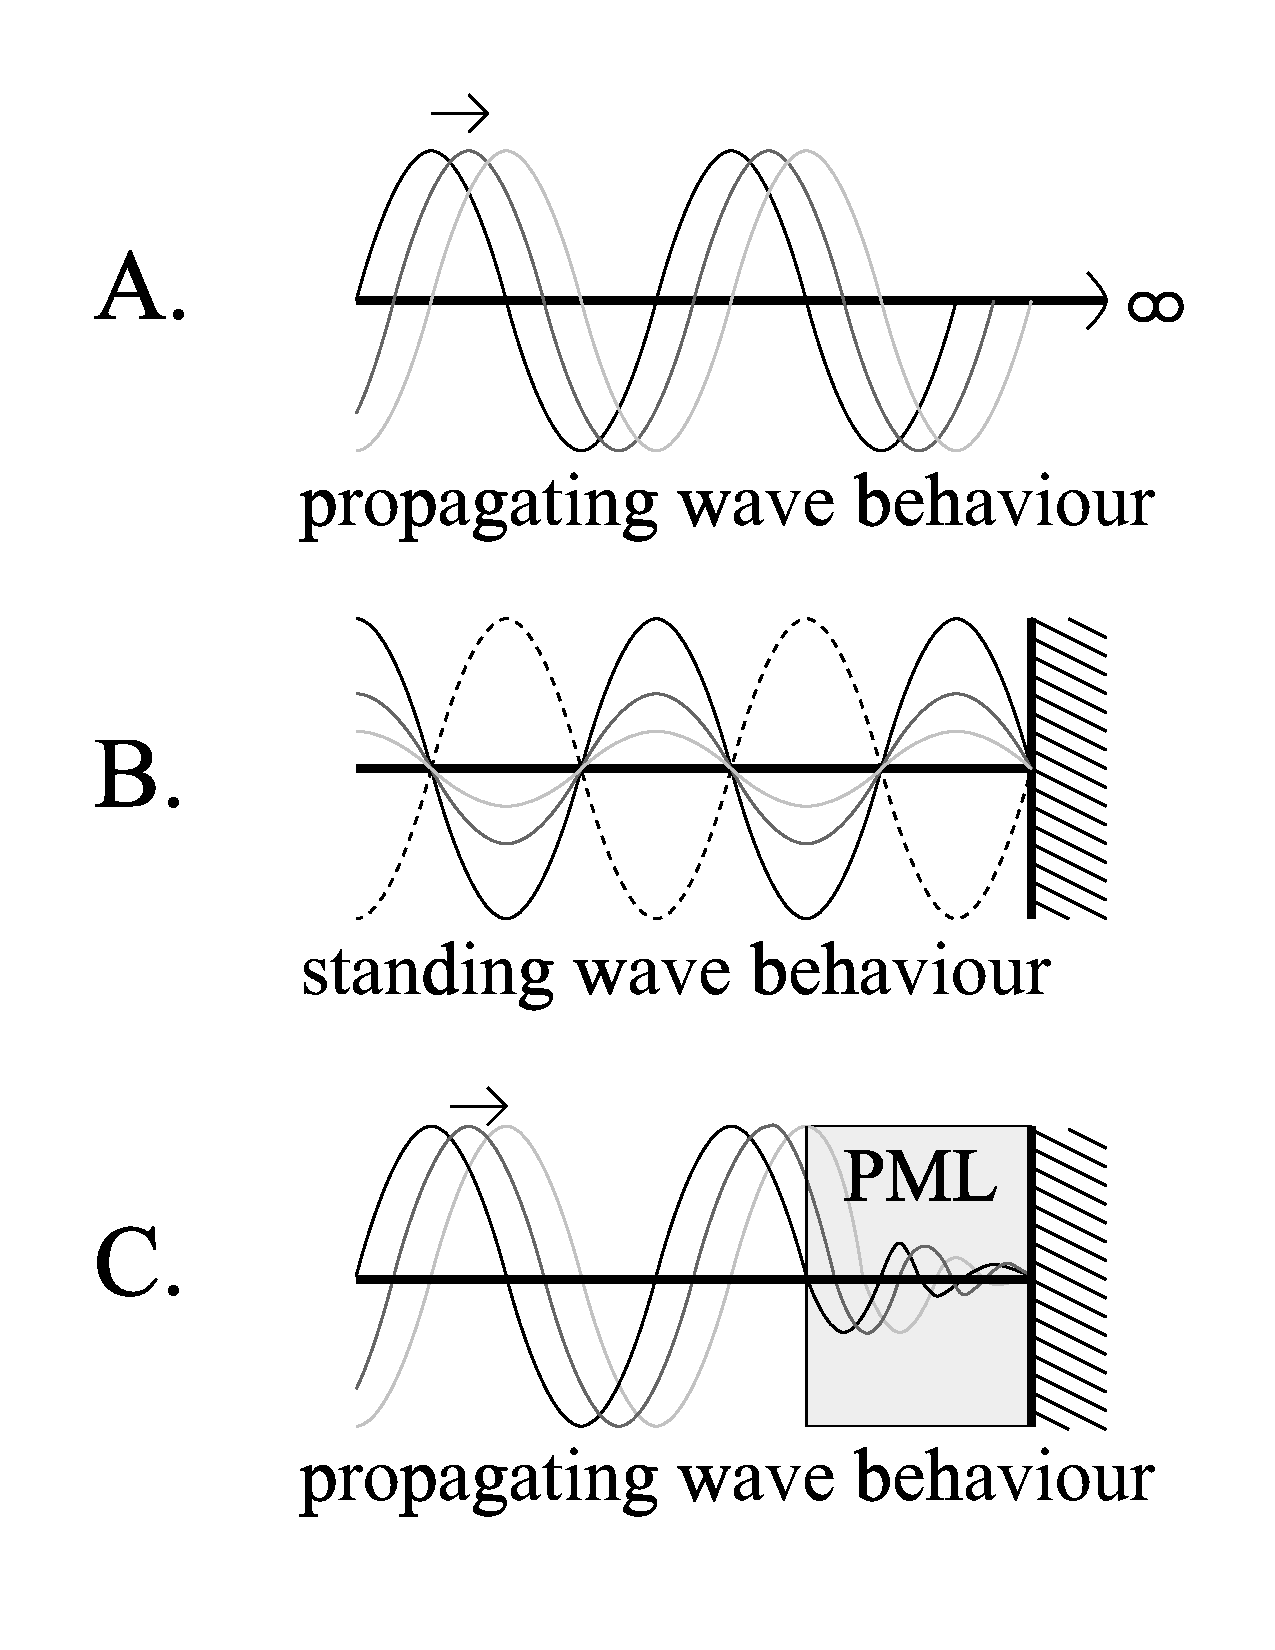
\includegraphics[trim = 0in 0in 0in 0in, clip, height=4in]{fig/propagatingwaves.pdf}
  \caption{Propagating Waves}
  \label{fig:PropagatingWaves}
  \end{minipage}
%\end{figure}
%\begin{figure}[htbp]
  \begin{minipage}{0.45\linewidth}
  \centering
  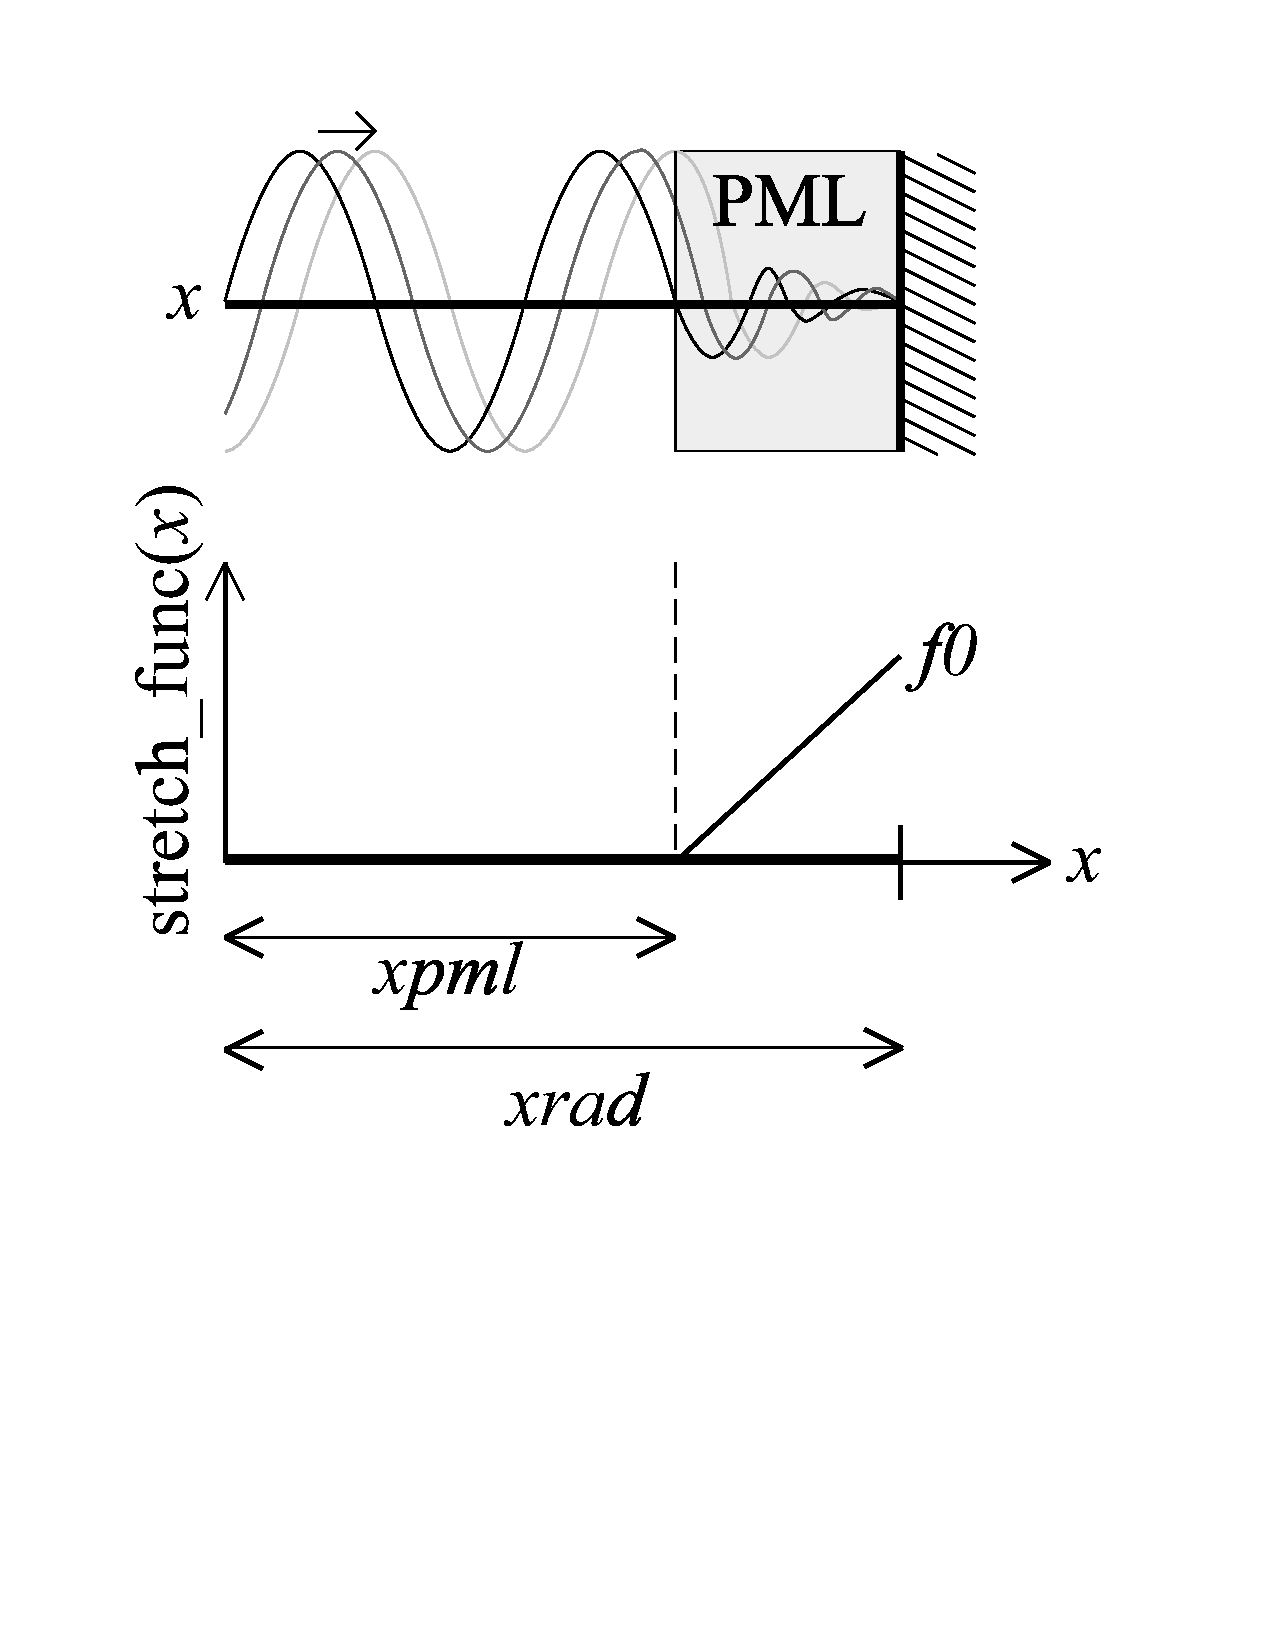
\includegraphics[trim = 0in 1in 0in 0in, clip, height=4in]{fig/1dpml.pdf}
  \caption{1D PML schematic}
  \label{fig:1DPMLSchematic}
  \end{minipage}
\end{figure}

\clearpage
\subsubsection*{Input file (LUA)}
\begin{flushleft}
  \textbf{Inputfile:}
  \ttt{\ttilde/hiqlab/models/tutorial/pml1d/pml1d.lua}\\
\end{flushleft}
\hspace{1in}
{\footnotesize
\listinginput[10]{1}{../../../models/tutorial/pml1d/pml1d.lua}
}

\clearpage
\begin{itemize}

  \item{\textbf{Construct element:}}
  First a material table \ttt{mtype} is defined. The
  required fields for a scalar static problem are 
  the Youngs modulus \ttt{E} and mass density \ttt{rho}.
  This material type, along with the string defining the 
  type of analysis is given to the command \ttt{make\_material\_s}
  which produces a scalar material.
  \begin{verbatim}
      etype = make_material_e( mtype, '1d');
  \end{verbatim}
  named \ttt{etype}.
  This element is used when elements are added to the \ttt{mesh}.

  \item{\textbf{Define PML parameter:}}
  The performance of the PML depends on the parameter \ttt{f0} and
  must be selected in accordance with the PML length.
  This value can be selected heuristically as shown in paper ???. 
  In general a long PML and large \ttt{f0} desired, though
  increasing the length will increase computational costs and 
  as will be seen in the example, increasing the \ttt{f0} without
  increasing the mesh density of the elements degrades performance.
  In MEMS applications a value of approximately 40 is observed to
  give standard performance.

  \item{\textbf{Define mesh using block command:}}
  The function \ttt{add\_block} adds a block of elements in the 
  range \ttt{[0, xrad]}. There are \ttt{num\_elem+1} nodes and 
  the elements have the order \ttt{order}.

  \item{\textbf{Define stretch function for PML:}}
  The stretch function to define the PML is defined here.
  The function must have the following structure, where
  the input is the physical coordinates of the mesh \ttt{x}, 
  and the output parameters are the stretching amount
  in each direction \ttt{sx}.
  \begin{verbatim}
     function stretch_function(x)
       -- compute sx
       return sx
     end
  \end{verbatim}

  \item{\textbf{Assign stretch function to element:}}
  The stretch function must be assigned to all elements that
  are defined as the PML region by the command,
  \begin{verbatim}
     etype:set_stretch(stretch_function)
  \end{verbatim}

  \item{\textbf{Define and assign boundary conditions:}}  
  A forced displacement boundary condition is set at the left end,
  and a fixed zero displacement boundary condition at the right end.

  Once the boundary condition function defined, it is assigned 
  to the mesh through the \ttt{set\_bc} command.

\end{itemize}

\clearpage
\subsubsection*{Solve harmonic problem (MATLAB)}
\begin{flushleft}
  \textbf{Inputfile:}
  \ttt{\ttilde/hiqlab/models/tutorial/pml1d/pml1d.m}\\
\end{flushleft}
\hspace{1in}
{\footnotesize
\listinginput[10]{1}{../../../models/tutorial/pml1d/pml1d.m}
}

\clearpage
Once the mesh is defined, the next step is to solve the problem.
This can be done both in Lua and MATLAB. Here we present the MATLAB
interface. 
The mesh obtained for this model is shown in 
Figure \ref{fig:PML1dMeshMATLAB}.

\begin{itemize}

  \item{\textbf{Define forcing frequency}}
  The computation conducted is a forced response. The 
  forcing frequency \ttt{w} is defined here in radians.

  \item{\textbf{Plot stretch function}}
  The stretch function should always be inspected for error.
  The function is visualized by the \ttt{plofield1d} command.
  This is done by assigning the string name of the stretch function, 
  in this case \ttt{stretch\_function}, to the field \ttt{cfields}
  in the optional structure \ttt{popt} and passing it to the 
  function \ttt{plotfield1d}. 

  \item{\textbf{Construct matrices and solve for harmonice displacements}}
  Here the matrices and forcing vectors are formed. The mathematical 
  structure of ordinary differential equation of the problem is
  \begin{eqnarray}
     \bfM\ddot{\bfu} + \bfK\bfu = \bff \nonumber
  \end{eqnarray} 
  By assuming harmonic displacements of the form,
  \begin{eqnarray}
     \bfu &=& \bfU \exp\left(iwt\right) \nonumber \\
     \bff &=& \bfF \exp\left(iwt\right) \nonumber
  \end{eqnarray}
  the equation,
  \begin{eqnarray}
    \bfU &=& \left(\bfK-w^2\bfM\right)^{-1}\bfF \nonumber
  \end{eqnarray}
  is obtained. 
  The function \ttt{harmonic\_state} solves this equation, given
  the forcing pattern $\bfF$.

  \item{\textbf{Display results}}
  The animation of the time-harmonic motion is displayed through
  the function \ttt{plotcycle1d}. (See section on plots for details).

\end{itemize}

\begin{figure}[htbp]
    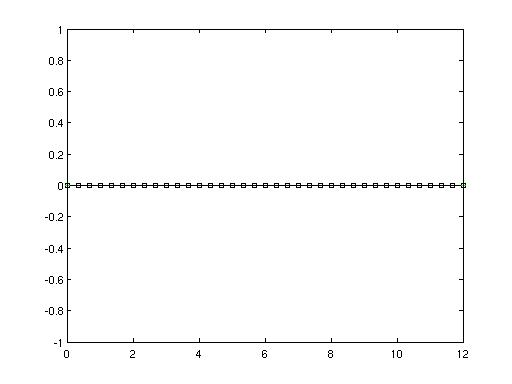
\includegraphics[width=\linewidth]{fig/pml1d_mesh_matlab.jpg}
    \caption{PML1d mesh from MATLAB}
    \label{fig:PML1dMeshMATLAB}
\end{figure}

\clearpage
\subsubsection*{Parametric study (MATLAB)}
Parametric study conducted by varying the variable 
\ttt{f0}. The stretch function values and mode shape plots
obtained for each case is shown in the figures.
For \ttt{f0=0} we see standing wave behavior, for \ttt{f0=40}
propagating wave behavior, and for \ttt{f0=4e6} again
standing wave behavior. 

\begin{figure}[htbp]
  \begin{minipage}{0.45\linewidth}
    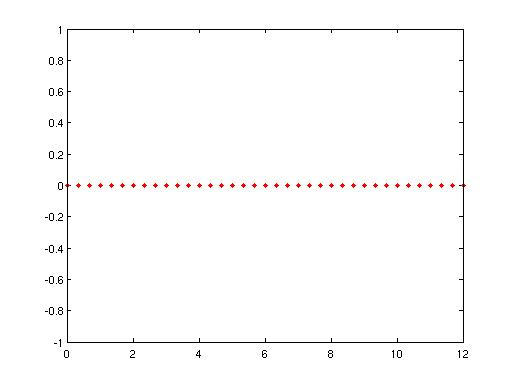
\includegraphics[width=\linewidth]{fig/pml1d_stretch0_matlab.jpg}
    \caption{PML1d stretch function from MATLAB(\ttt{f0=0})}
    \label{fig:PML1dStretchFunction0MATLAB}
  \end{minipage}
  \hfill
  \begin{minipage}{0.45\linewidth}
    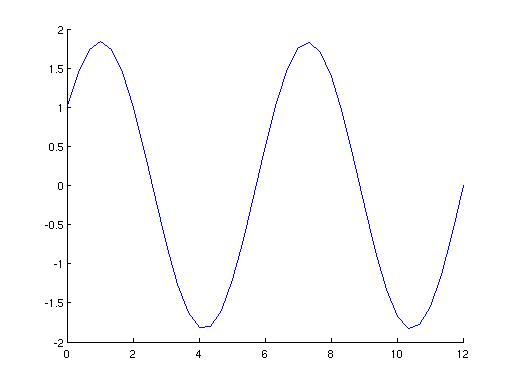
\includegraphics[width=\linewidth]{fig/pml1d_mode0_matlab.jpg}
    \caption{PML1d mode shape from MATLAB(\ttt{f0=0})}
    \label{fig:PML1dModeShape0MATLAB}
  \end{minipage}
  \begin{minipage}{0.45\linewidth}
    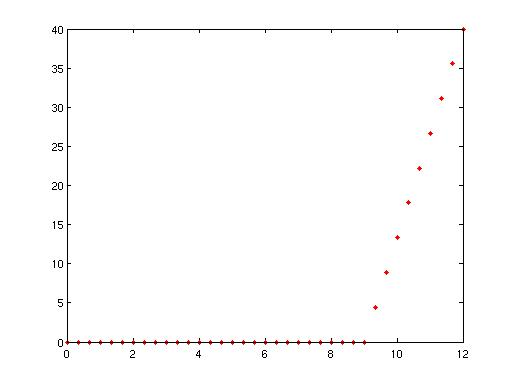
\includegraphics[width=\linewidth]{fig/pml1d_stretch40_matlab.jpg}
    \caption{PML1d stretch function from MATLAB(\ttt{f0=40})}
    \label{fig:PML1dStretchFunction40MATLAB}
  \end{minipage}
  \hfill
  \begin{minipage}{0.45\linewidth}
    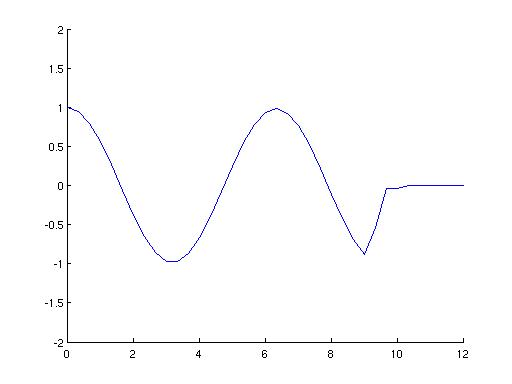
\includegraphics[width=\linewidth]{fig/pml1d_mode40_matlab.jpg}
    \caption{PML1d mode shape from MATLAB(\ttt{f0=40})}
    \label{fig:PML1dModeShape40MATLAB}
  \end{minipage}
  \begin{minipage}{0.45\linewidth}
    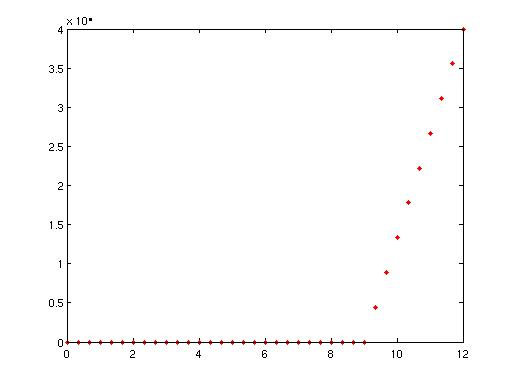
\includegraphics[width=\linewidth]{fig/pml1d_stretch4e6_matlab.jpg}
    \caption{PML1d stretch function from MATLAB(\ttt{f0=4e6})}
    \label{fig:PML1dStretchFunction4e6MATLAB}
  \end{minipage}
  \hfill
  \begin{minipage}{0.45\linewidth}
    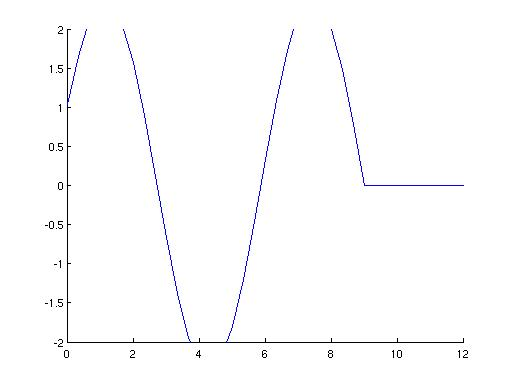
\includegraphics[width=\linewidth]{fig/pml1d_mode4e6_matlab.jpg}
    \caption{PML1d mode shape from MATLAB(\ttt{f0=4e6})}
    \label{fig:PML1dModeShape4e6MATLAB}
  \end{minipage}
\end{figure}

\clearpage
\subsection{2D waves}
\begin{flushleft}
  \textbf{Inputfile:}
  \ttt{\ttilde/hiqlab/models/tutorial/pml2d}\\
  \textbf{Lua features introduced:pml\_blocks2d}\\
  \textbf{MATLAB features introduced:}\\
  \ttt{plotfield2d, plotcycle2d}
\end{flushleft}
This example illustrates basic anchor loss
modeling using Perfect Matched Layers for the 
2D dimensional case. Two wave problems can
be considered for the 2 dimensional case, the
scalar wave and elastic wave. Both cases take
the same form for the stretch function required
to implement the PML. The functions are linear 
as in the 1 dimensional case, and their form
is shown in the schematic in Figure
\ref{fig:PML2dSchematic}. The mesh and stretch
function for both cases are shown in 
Figure \ref{fig:PML2dMeshMATLAB} and 
Figure \ref{fig:PML2dStretchFunctionMATLAB}.

\begin{figure}[htbp]
  \centering
  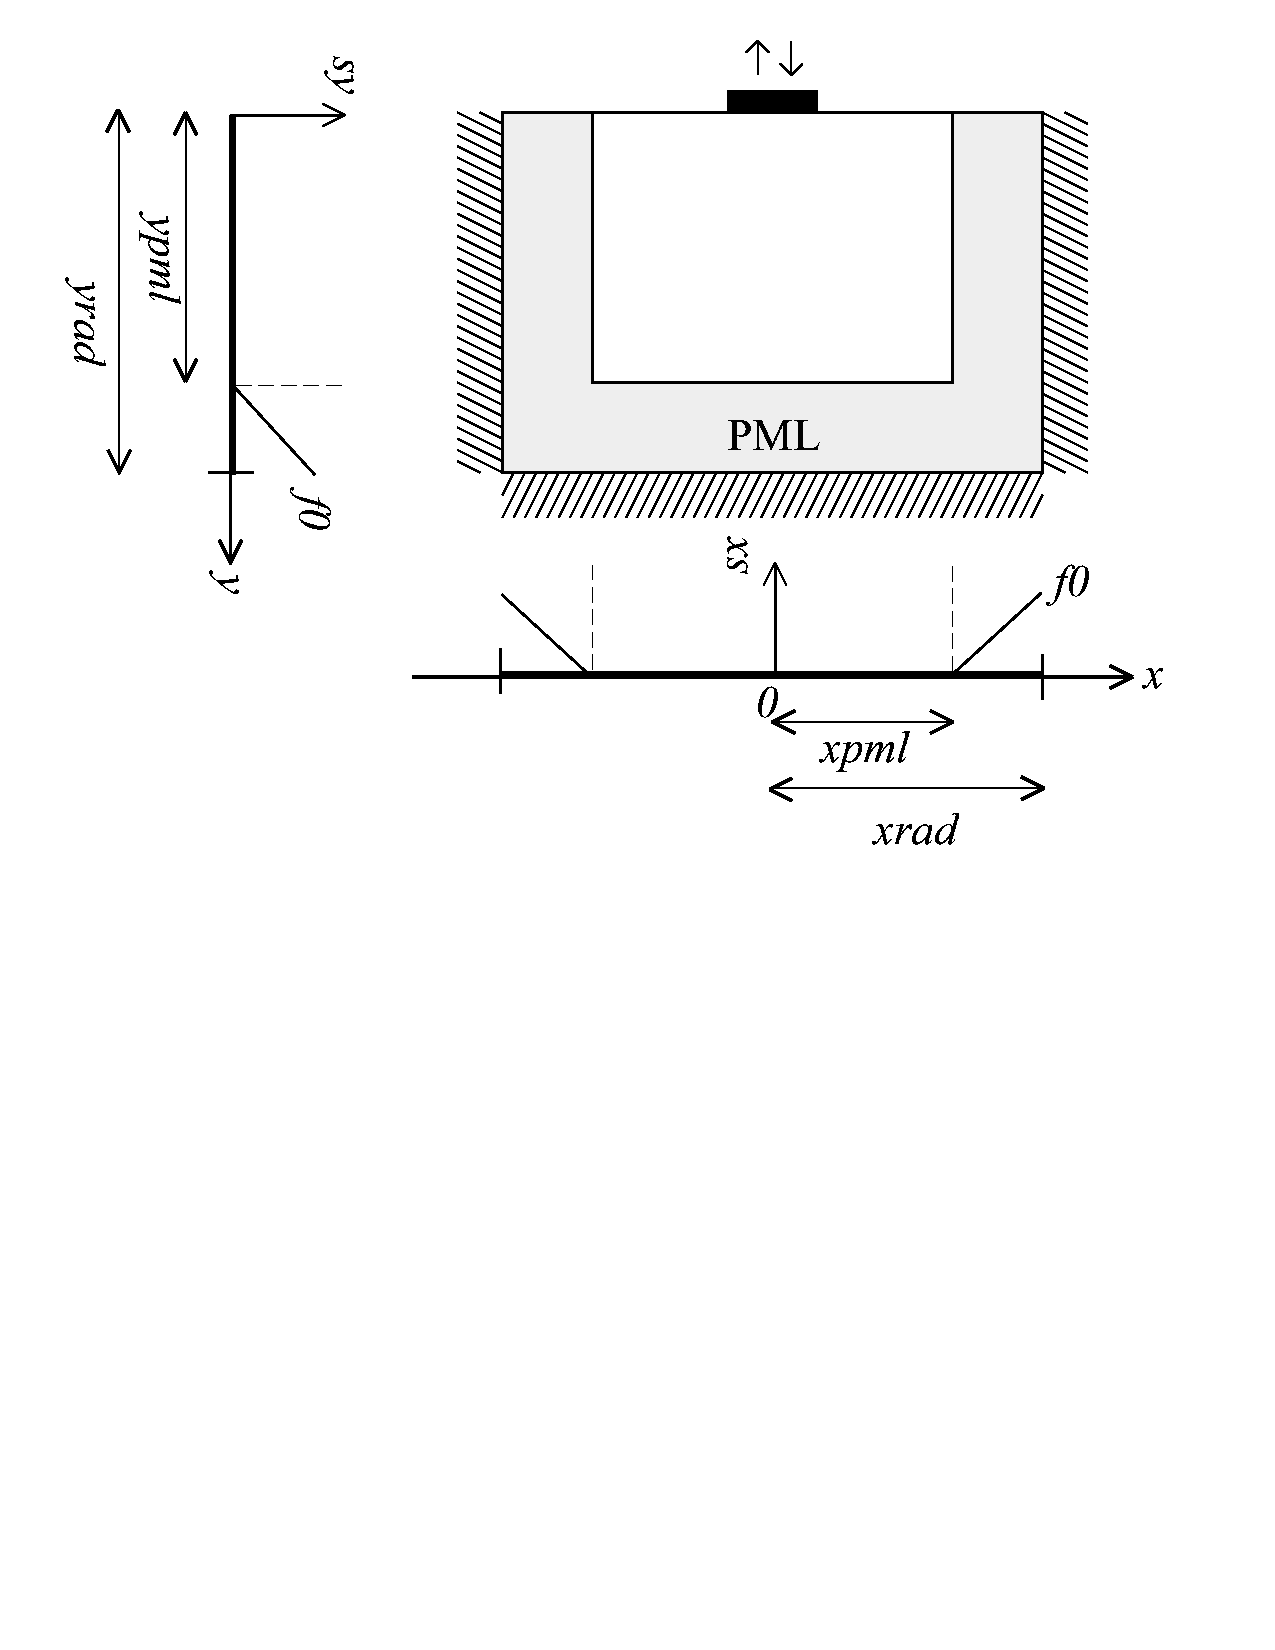
\includegraphics[trim = 0in 5in 0in 0in, clip, height=3.5in]{fig/2dpml.pdf}
  \caption{PML2d schematic}
  \label{fig:PML2dSchematic}
%\end{figure}
%\begin{figure}[htbp]
  \begin{minipage}{0.45\linewidth}
    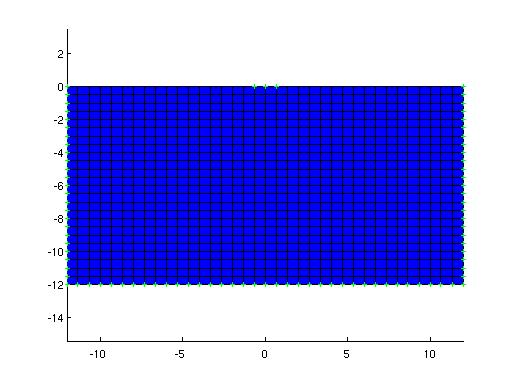
\includegraphics[width=\linewidth]{fig/pml2d_mesh_matlab.jpg}
    \caption{PML2d mesh from MATLAB}
    \label{fig:PML2dMeshMATLAB}
  \end{minipage}
  \hfill
  \begin{minipage}{0.45\linewidth}
    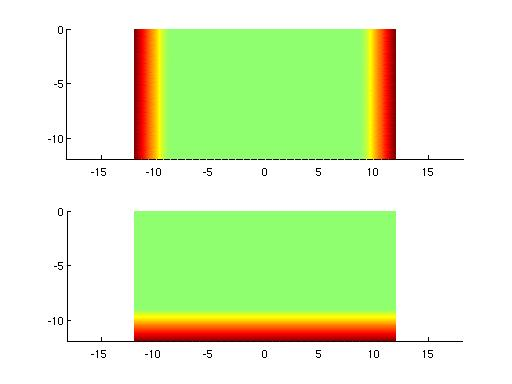
\includegraphics[width=\linewidth]{fig/pml2d_stretch_matlab.jpg}
    \caption{PML2d stretch function from MATLAB(\ttt{f0=40})}
    \label{fig:PML2dStretchFunctionMATLAB}
  \end{minipage}
\end{figure}

\clearpage
\subsubsection{Elastic waves in a half space}
\subsubsection*{Input file (LUA)}
\begin{flushleft}
  \textbf{Inputfile:}
  \ttt{\ttilde/hiqlab/models/tutorial/pml2d/pml2d.lua}\\
\end{flushleft}
\hspace{1in}
{\footnotesize
\listinginput[10]{1}{../../../models/tutorial/pml2d/pml2d.lua}
}

\clearpage
There is an additional file which uses the \ttt{pml\_blocks2d}
command to simply construct the pml anchor block.

\begin{itemize}

  \item{\textbf{Define Forcing parameters:}}
  Parameter \ttt{a} defines a pulling type of motion and 
  \ttt{b} a rocking type of motion. An example of 
  each is shown in the figures.

  \item{\textbf{Define stretch function for PML:}}
  The stretch function to define the PML is defined here.
  The function must have the following structure, where
  the input is the physical coordinates of the mesh \ttt{x,y}, 
  and the output parameters are the stretching amount
  in each direction \ttt{sx,sy}.
  \begin{verbatim}
     function stretch_function(x,y)
       -- compute sx,sy
       return sx,sy
     end
  \end{verbatim}
  The equations are,
  \begin{eqnarray}
  \text{sx}
        &=& \text{max}\left(0, \text{f0} \frac{\text{abs(x)-xpml}}{\text{xrad-xpml}}\right) \nonumber \\
  \text{sy}
        &=& \text{max}\left(0, \text{f0} \frac{\text{abs(y)-ypml}}{\text{yrad-ypml}}\right) \nonumber 
  \end{eqnarray}

  \item{\textbf{Assign stretch function to element:}}
  The stretch function must be assigned to all elements that
  are defined as the PML region by the command,
  \begin{verbatim}
     etype:set_stretch(stretch_function)
  \end{verbatim}

  \item{\textbf{Define and assign boundary conditions:}}  
  A forced displacement boundary condition is set at the middle with
  width 2, and fixed zero displacement boundary conditions are 
  defined on the bottom, left, and right edges.

  Once the boundary condition function is defined, it is assigned 
  to the mesh through the \ttt{set\_bc} command.

\end{itemize}

\clearpage
\subsubsection*{Input file using \ttt{pml\_blocks2d}(LUA)}
\begin{flushleft}
  \textbf{Inputfile:}
  \ttt{\ttilde/hiqlab/models/tutorial/pml2d/pml2d\_pmlblocks2d.lua}\\
\end{flushleft}
\hspace{1in}
{\footnotesize
\listinginput[10]{1}{../../../models/tutorial/pml2d/pml2d_pmlblocks2d.lua}
}

\clearpage
By using the function \ttt{pml\_blocks2d} this becomes,
\begin{itemize}

  \item{\textbf{Define pml block by function:}}
  The function creates a block of pml and returns the boundary 
  condition on the perimeter of the block \ttt{bc\_pmlfunc} and 
  the required stretch function \ttt{pml\_pmlfunc}. The input
  arguments are the nodes on the interface that the pml block is 
  to connect to. In this case nodes $(x,y) = (-1,0),(1,0)$. The
  first argument requires the x positions of these nodes and the 
  second the y positions. The third 2 denotes the degrees of freedom
  clamped at the edge by the boundary condition. In this case it is
  2 since it is a purely mechanical problem. The next two argument
  define the width and height of the pml block. \ttt{dpml} defines
  the depth of the pml layer from the fixed edges, \ttt{f0} is the
  damping parameter, \ttt{etype} the type of element used to construct
  the block, \ttt{order} is the order of interpolation, and 
  \ttt{densex,densey} are the approximate size of the elements in the 
  x and y direction.

  \item{\textbf{Set boundary condition}}
  In this case two boundary conditions must be set. One for the 
  forced boundary condition \ttt{bc\_function}, and the other for
  the anchor boundary condition \ttt{bc\_pmlfunc}. Thus a table
  bracketed by \{ and \} is passed to the function \ttt{set\_bc}.

\end{itemize}

\clearpage
\subsubsection*{Solve harmonic problem (MATLAB)}
\begin{flushleft}
  \textbf{Inputfile:}
  \ttt{\ttilde/hiqlab/models/tutorial/pml2d/pml2d.m}\\
\end{flushleft}
\hspace{1in}
{\footnotesize
\listinginput[10]{1}{../../../models/tutorial/pml2d/pml2d.m}
}

\clearpage
Once the mesh is defined, the next step is to solve the problem.
This can be done both in Lua and MATLAB. Here we present the MATLAB
interface. 
The mesh obtained for this model is shown in 
Figure \ref{fig:PML2dMeshMATLAB}.

\begin{itemize}

  \item{\textbf{Define forcing frequency}}
  The computation conducted is a forced response. The 
  forcing frequency \ttt{w} is defined here in radians.

  \item{\textbf{Define forcing pattern}}
  Additional parameters to define the forcing pattern are passed.
  The difference between these are shown in the figures.
  
  \item{\textbf{Plot stretch function}}
  The stretch function should always be inspected for error.
  The function is visualized by the \ttt{plofield1d} command.
  This is done by assigning the string name of the stretch function, 
  in this case \ttt{stretch\_function}, to the field \ttt{cfields}
  in the optional structure \ttt{popt} and passing it to the 
  function \ttt{plotfield2d}. 

  \item{\textbf{Display results}}
  The animation of the time-harmonic motion is displayed through
  the function \ttt{plotcycle2d}. (See section on plots for details).

\end{itemize}

\begin{figure}[htbp]
    \centering
    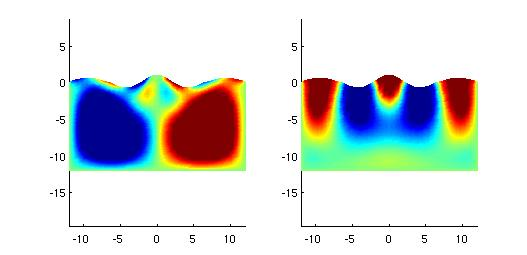
\includegraphics[width=0.7\linewidth]{fig/pml2d_mode0_matlab.jpg}
    \caption{PML2d mode shape from MATLAB(\ttt{f0=0})}
    \label{fig:PML2dModeShape0MATLAB}
    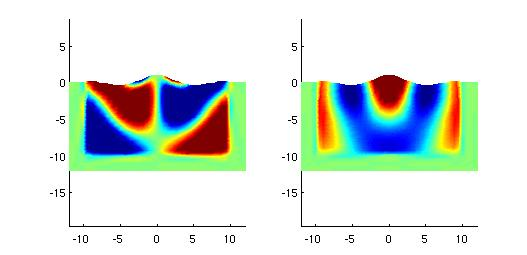
\includegraphics[width=0.7\linewidth]{fig/pml2d_mode40_matlab.jpg}
    \caption{PML2d mode shape from MATLAB(\ttt{f0=40})}
    \label{fig:PML2dModeShape40MATLAB}
    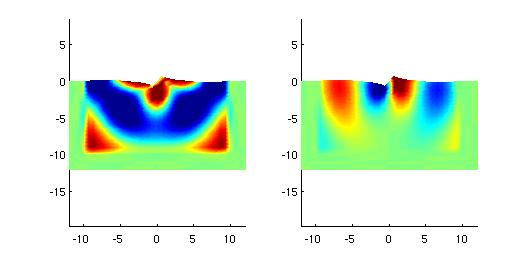
\includegraphics[width=0.7\linewidth]{fig/pml2d_mode40r_matlab.jpg}
    \caption{PML2d rocking mode shape from MATLAB(\ttt{f0=40})}
    \label{fig:PML2dModeShape40RockingMATLAB}
\end{figure}

\clearpage
\subsubsection{Scalar waves in a half space}
Since this is almost identical to the elastic case we
will only present the Lua input file and corresponding 
Matlab file.

\clearpage
\subsubsection*{Input file (LUA)}
\begin{flushleft}
  \textbf{Inputfile:}
  \ttt{\ttilde/hiqlab/models/tutorial/pml2d/pml2ds.lua}\\
\end{flushleft}
\hspace{1in}
{\footnotesize
\listinginput[10]{1}{../../../models/tutorial/pml2d/pml2ds.lua}
}

\clearpage
\subsubsection*{Solve harmonic problem (MATLAB)}
\begin{flushleft}
  \textbf{Inputfile:}
  \ttt{\ttilde/hiqlab/models/tutorial/pml2d/pml2ds.m}\\
\end{flushleft}
\hspace{1in}
{\footnotesize
\listinginput[10]{1}{../../../models/tutorial/pml2d/pml2ds.m}
}


\clearpage
\subsection{Axis-symmetric waves}
\begin{flushleft}
  \textbf{Inputfile:}
  \ttt{\ttilde/hiqlab/models/tutorial/pmlaxis}\\
  \textbf{Lua features introduced:}\\
  \textbf{MATLAB features introduced:}
\end{flushleft}
This example illustrates basic anchor loss
modeling using Perfect Matched Layers for the 
axis symmetric dimensional case. Two wave problems can
be considered for the 2 dimensional case, the
scalar wave and elastic wave. Both cases take
the same form for the stretch function required
to implement the PML. The functions are linear 
as in the 1 dimensional case, and their form
is shown in the schematic in Figure
\ref{fig:PMLAxisSchematic}. The mesh and stretch
function for both cases are shown in 
Figure \ref{fig:PMLAxisMeshMATLAB} and 
Figure \ref{fig:PMLAxisStretchFunctionMATLAB}.

\begin{figure}[htbp]
  \centering
  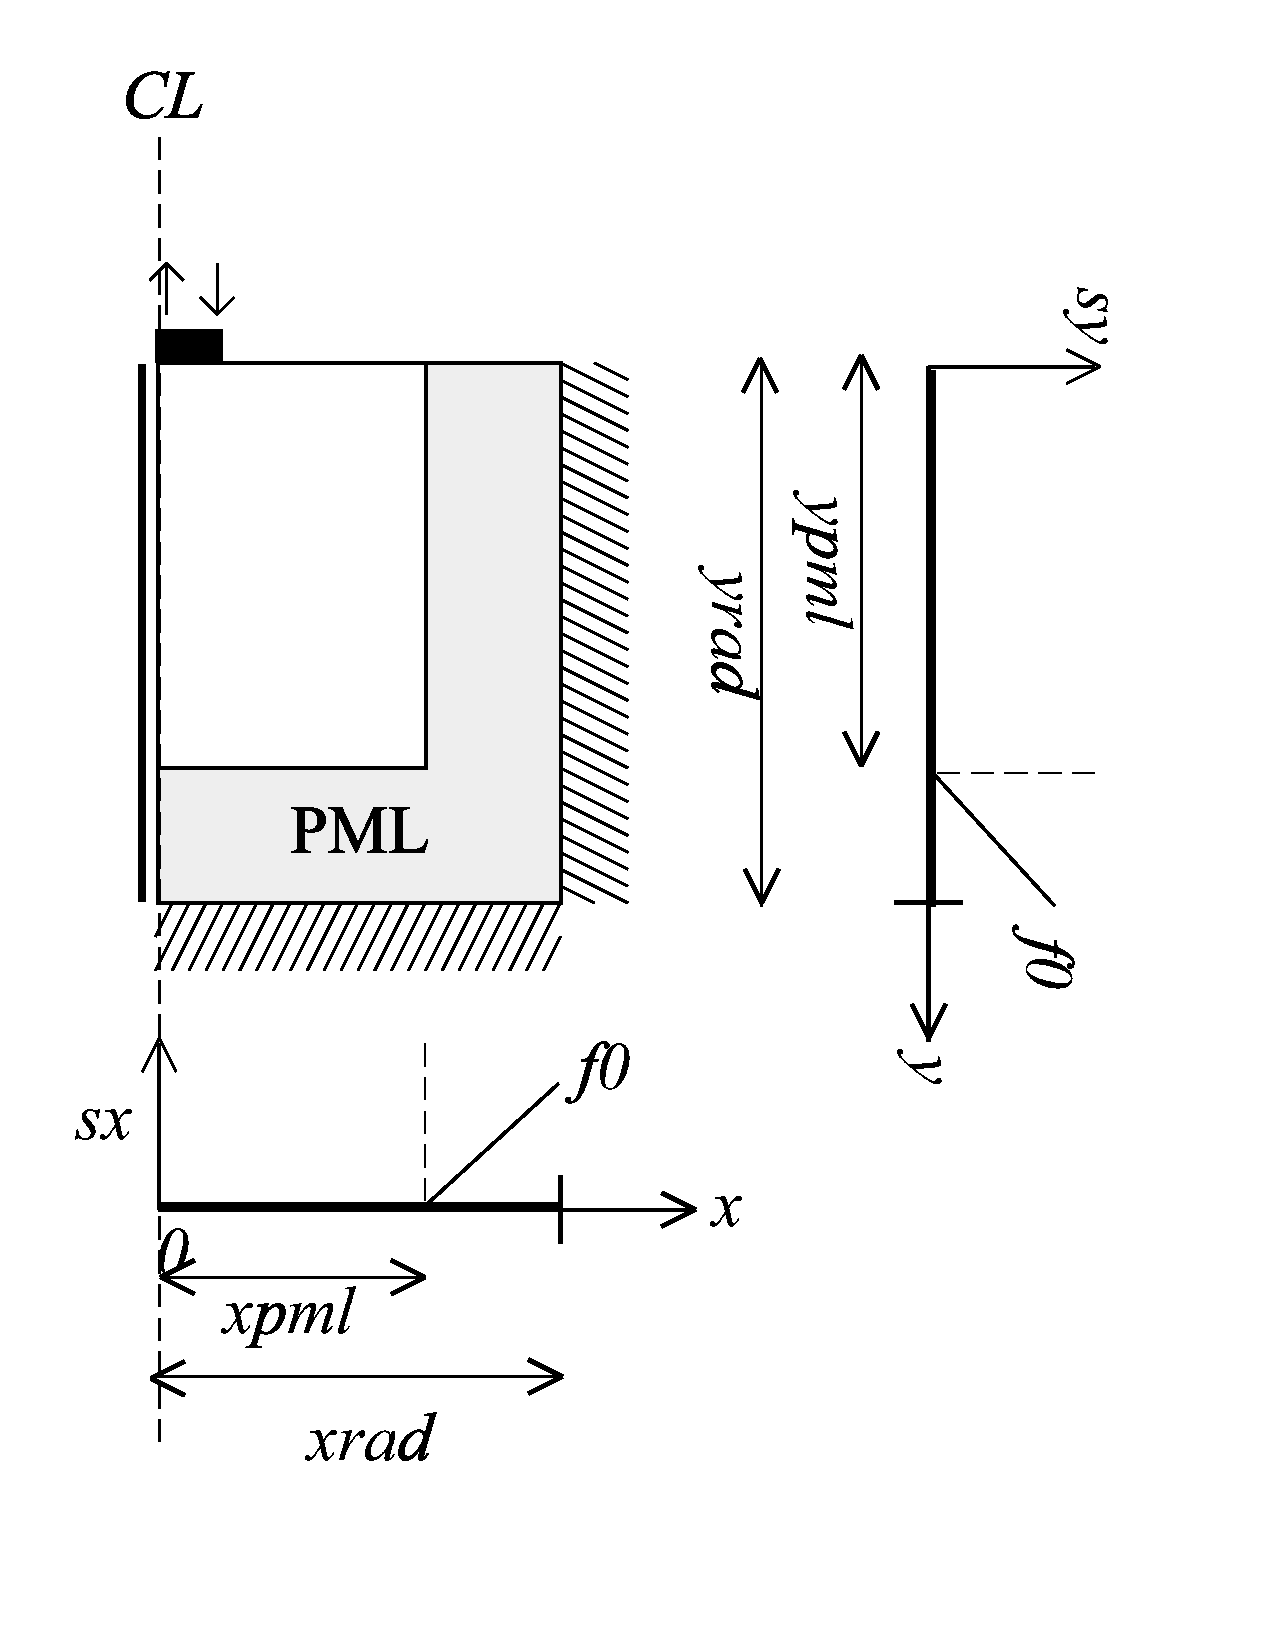
\includegraphics[trim = 0in 2in 0in 0in, clip, height=4in]{fig/2daxispml.pdf}
  \caption{PML Axis Schematic}
  \label{fig:PMLAxisSchematic}
%\end{figure}
%\begin{figure}[htbp]
  \begin{minipage}{0.45\linewidth}
    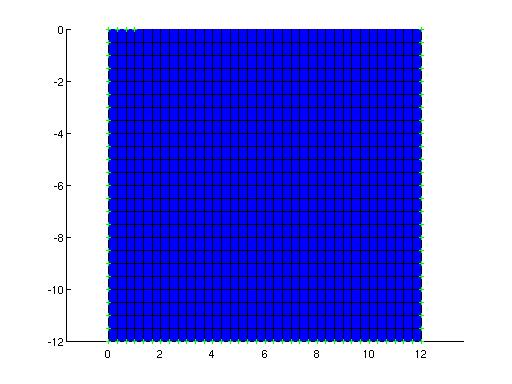
\includegraphics[width=\linewidth]{fig/pmlaxis_mesh_matlab.jpg}
    \caption{PMLAxis mesh from MATLAB}
    \label{fig:PMLAxisMeshMATLAB}
  \end{minipage}
  \hfill
  \begin{minipage}{0.45\linewidth}
    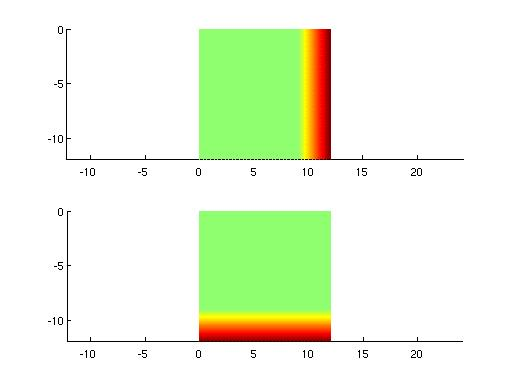
\includegraphics[width=\linewidth]{fig/pmlaxis_stretch_matlab.jpg}
    \caption{PMLAxis stretch function from MATLAB(\ttt{f0=40})}
    \label{fig:PMLAxisStretchFunctionMATLAB}
  \end{minipage}
\end{figure}


\clearpage
\subsubsection{Elastic waves in a half space}
Since this is almost identical to the 2d case we
will only present the Lua input file and corresponding 
Matlab file. 

\clearpage
\subsubsection*{Input file (LUA)}
\begin{flushleft}
  \textbf{Inputfile:}
  \ttt{\ttilde/hiqlab/models/tutorial/pmlaxis/pmlaxis.lua}\\
\end{flushleft}
\hspace{1in}
{\footnotesize
\listinginput[10]{1}{../../../models/tutorial/pmlaxis/pmlaxis.lua}
}

\clearpage
\subsubsection*{Solve harmonic problem (MATLAB)}
\begin{flushleft}
  \textbf{Inputfile:}
  \ttt{\ttilde/hiqlab/models/tutorial/pmlaxis/pmlaxis.m}\\
\end{flushleft}
\hspace{1in}
{\footnotesize
\listinginput[10]{1}{../../../models/tutorial/pmlaxis/pmlaxis.m}
}


\clearpage
\subsubsection{Scalar waves in a half space}
Since this is almost identical to the 2D case we
will only present the Lua input file and corresponding 
Matlab file. 

\clearpage
\subsubsection*{Input file (LUA)}
\begin{flushleft}
  \textbf{Inputfile:}
  \ttt{\ttilde/hiqlab/models/tutorial/pmlaxis/pmlaxis\_s.lua}\\
\end{flushleft}
\hspace{1in}
{\footnotesize
\listinginput[10]{1}{../../../models/tutorial/pmlaxis/pmlaxis_s.lua}
}

\clearpage
\subsubsection*{Solve harmonic problem (MATLAB)}
\begin{flushleft}
  \textbf{Inputfile:}
  \ttt{\ttilde/hiqlab/models/tutorial/pmlaxis/pmlaxis\_s.m}\\
\end{flushleft}
\hspace{1in}
{\footnotesize
\listinginput[10]{1}{../../../models/tutorial/pmlaxis/pmlaxis_s.m}
}


\clearpage
\section{Coupled analysis: MEMS cantilever beam}
In this section the MEMS cantilever beam is used to introduce
the coupled analysis features that exist. Three types of 
coupled problems are solved,
\begin{enumerate}
\item Mechanical problem
\item Thermoelastic problem
\item Electromechanical problem
\end{enumerate} 
For each, three types of analyses are conducted,
\begin{enumerate}
\item Static analysis              (\ttt{mems\_cant\_sta.m})
\item Dynamic modal analysis       (\ttt{mems\_cant\_dyn.m})
\item Transfer function evaluation (\ttt{mems\_cant\_tra.m})
\end{enumerate} 
where the file in the parantheses denotes the MATLAB execution file.
The Lua inputfiles along with the a short description of the aim of the
example is summarized in Table~\ref{table:LuaFilesForMEMSBeam}.

\begin{table}[htbp]
\centering
\caption{Lua files for a MEMS beam}
\label{table:LuaFilesForMEMSBeam}
\begin{tabular}{|l|l|l|m{2.5in}|}
\hline
Problem domain    & Lua filename                     
& MATLAB file       & Objective \\
\hhline{|=|=|=|=|}
Mechanical        & \ttt{mems\_cant\_m.lua}          
& \ttt{sta,dyn,tra} & simple mechanical problem \\
                  & \ttt{mems\_cant\_m\_nondim.lua}  
& \ttt{sta,dyn,tra} & nondimensionalization of problem \\
                  & \ttt{mems\_cant\_wa\_m.lua}      
& \ttt{sta,dyn,tra} & mechanical problem with anchor loss \\
\hline
Thermoelastic     & \ttt{mems\_cant\_te\_sta.lua}    
& \ttt{sta}         & simple static thermoelastic problem \\
                  & \ttt{mems\_cant\_te.lua}         
& \ttt{dyn,tra}     & thermoelastic problem with anchor loss \\
                  & \ttt{mems\_cant\_wa\_te\_sta.lua}
& \ttt{sta}         & static thermoelastic problem with anchor \\
                  & \ttt{mems\_cant\_wa\_te.lua}     
& \ttt{dyn,tra}     & thermoelastic problem with anchor loss \\
\hline
Electromechanical & \ttt{mems\_cant\_em.lua}         
& \ttt{sta,dyn,tra} & simple electromechanical problem \\
\hline
\end{tabular}
\end{table}

Throughout this section, the user is assumed to have worked through 
the previous two sections. Minor details of the Lua input files and 
MATLAB script files are omitted. 

\clearpage
\subsection{Mechanical analysis}
\begin{flushleft}
  \textbf{Inputfile:}
  \ttt{\ttilde/hiqlab/models/tutorial/mems\_cantilever\_beam}\\
  \textbf{Lua features introduced:}
  \ttt{mech\_nondim}(Non-dimensionalization), 
  material database in \ttt{'materials.lua'},
  \ttt{get\_dim\_scale}\\
  \textbf{MATLAB features introduced:}
  \ttt{Mesh\_get\_x, Mesh\_get\_disp, Mesh\_get\_sense\_disp,
       Mesh\_get\_u, Mesh\_get\_sense\_u, mechmode, second\_order\_bode,
       Mesh\_get\_drive\_f, Mesh\_get\_sense\_u, plot\_bode}  
\end{flushleft}
This example is used to illustrate the basic analysis methods,
the procedure for nondimensionalization and methods to extract
useful information from the analysis. A schematic of the cantilever
is shown in Figure~\ref{fig:MEMSCantileverBeam_Mech}. The beam thickness
\ttt{t} is considered to be small compared to the length \ttt{l} and
width \ttt{w}, which justifies the plane stress analysis conducted.
A point load of \ttt{P} is applied for the static analysis. For the
transfer function evaluation, the beam is forced at this tip and the
displacement is also sensed at this point.

\begin{figure}[htbp]
\centering
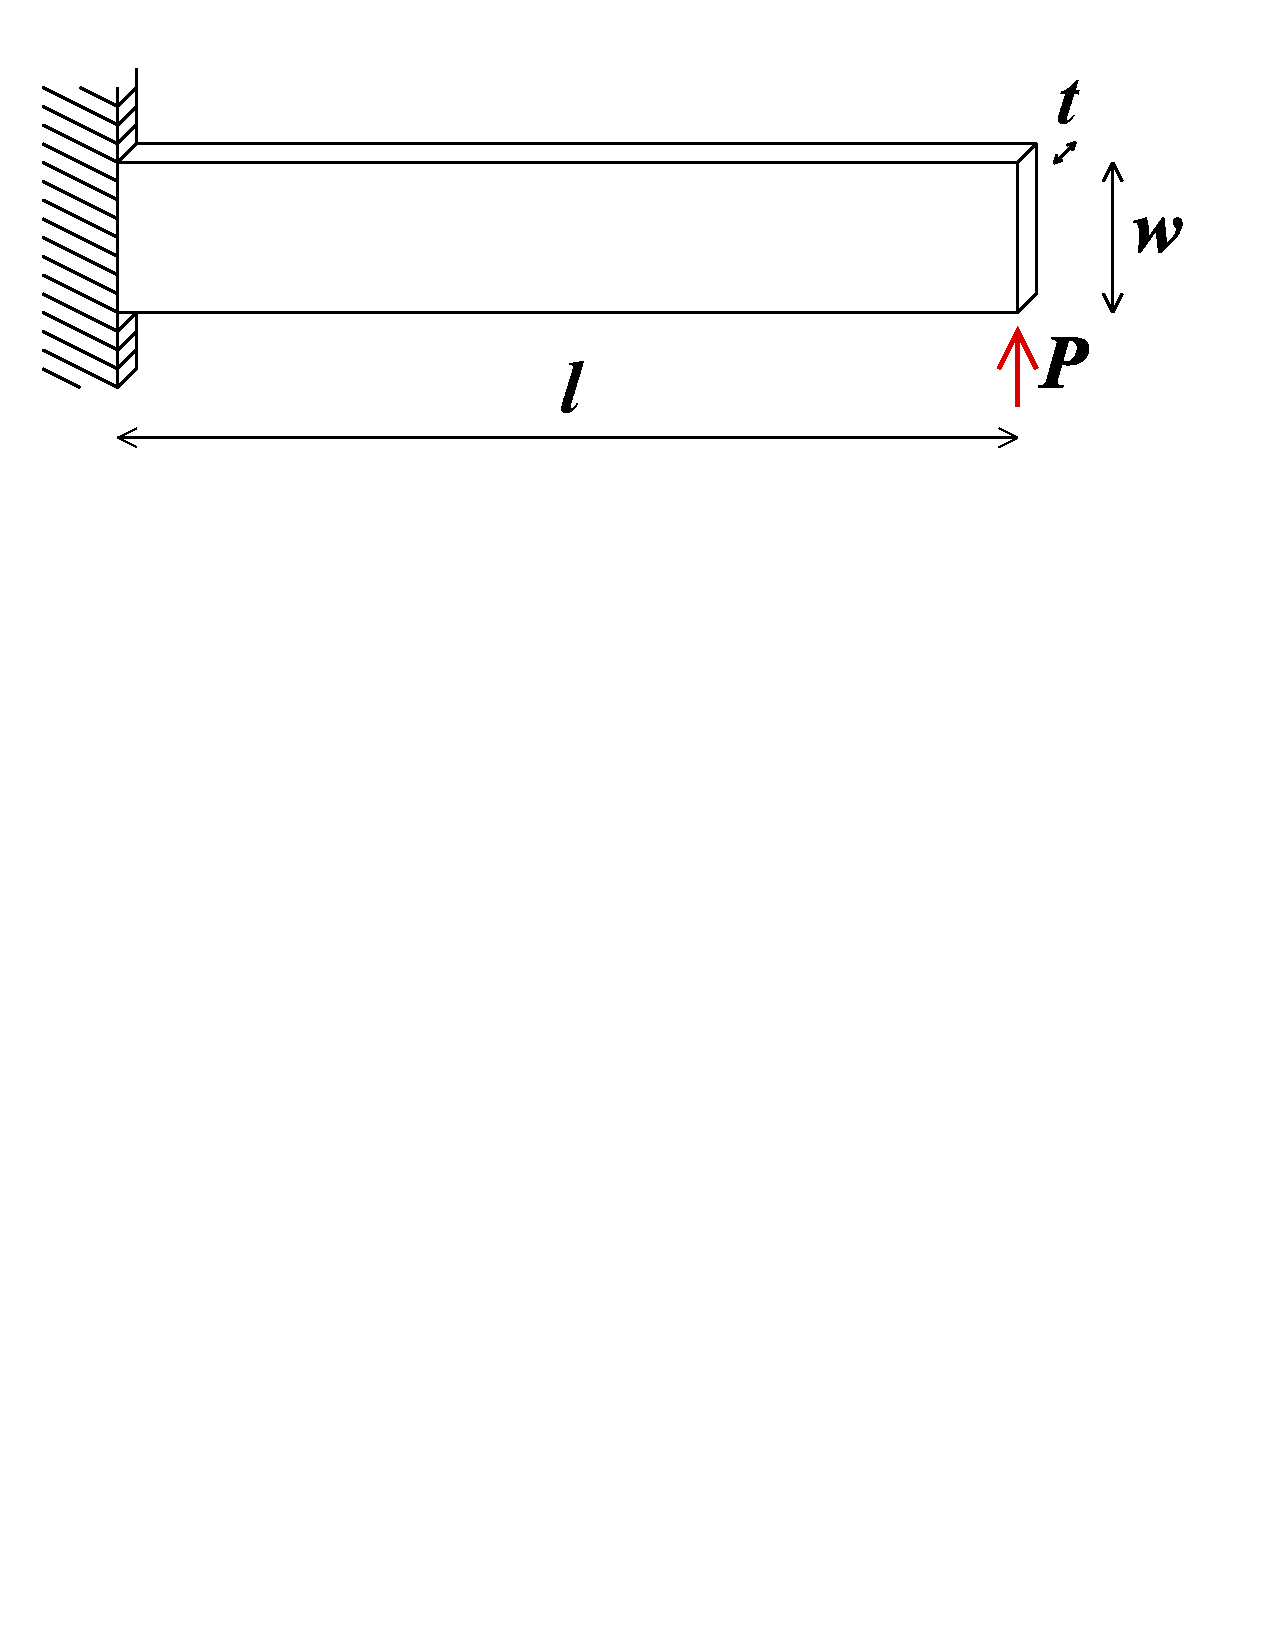
\includegraphics[trim = 0in 7in 0.5in 0in, clip, height = 2in]{fig/memscantileverbeam_mech.pdf}
\caption{Schematic of the MEMS cantilever beam}
\label{fig:MEMSCantileverBeam_Mech}
\end{figure}

\clearpage
\subsubsection*{Dimensional input file (LUA)}
\begin{flushleft}
  \textbf{Inputfile:}
  \ttt{\ttilde/hiqlab/models/tutorial/mems\_cantilever\_beam/mems\_cant\_m.lua}
\end{flushleft}
\hspace{1in}
{\footnotesize
\listinginput[10]{1}{../../../models/tutorial/mems_cantilever_beam/mems_cant_m.lua}
}

\clearpage
The analysis is conducted in dimensional form as opposed to the
Lua input file introduced in the next section.

\begin{itemize}

  \item{\textbf{Define order and approximate size of element :}}
  The default order of interpolation can be defined by a variable named
  \ttt{order}. When elements are produced by block generation without
  specification of the order of interpolation, this variable is used.
  Additionally it is convenient to set this parameter globally to
  control the interpolation of all elements.

  Similarly, the default approximate size of the elements produced by
  block generation are defined by the variable \ttt{dense}. 

  \item{\textbf{Define geometry of domain:}}
  The additional variable \ttt{t} is set for the thickness.
  Though this analysis is 2D, this variable is required to 
  define forces.

  \item{\textbf{Define force at the tip:}}
  The force is defined here not as a force per length. Thus
  when the force boundary conditions are applied, it will be
  divided by the thickness to obtain the force per unit length.  

  \item{\textbf{Define element type:}}
  Here we use the material database library. The material 
  parameters are set in the file \ttt{materials.lua} located
  in the \ttt{models} directory. See ??? for details.

\begin{verbatim}
        mtype = 'silicon2'
\end{verbatim}

  \item{\textbf{Define boundary condition:}}
  As noted above, the force boundary conditions are applied per
  unit length, since this is 2D analysis.

\begin{verbatim}
     mesheq( y, -w/2) then return ' f',  P/t; end
\end{verbatim}

  \item{\textbf{Define a sensing function to evaluate tip displacement:}}
  Displacements at nodes can be extracted by searching for the id of the
  node of interest from the nodal array. This process can be tedious when
  the number of nodes increases. As in the case of boundary conditions,
  one can extract the information of a specific node by a function of
  the form exactly the same as the boundary condition.

  The \ttt{' u'} denotes that the displacement in the $y$ direction 
  is what we would like to extract from the node. The $1$ denotes that
  we would like this value multiplied by unity. By invoking this function
  through MATLAB, a sensing vector is produced, with which the inner 
  product with displacement vector results in the desired quantity. 

  \item{\textbf{Define a sensing and forcing functions for producing 
                                                      a bode plott:}}
  As in the prevous function definition, these functions are used to 
  define the forcing and sensing patterns used to generate the bode plot.

  In the definition of the force function, the force $P$ has again been
  modified appropriately to reflect the 2D analysis.

\end{itemize}


\clearpage
\subsubsection*{Construct non-dimensional input file (LUA)}
\begin{flushleft}
  \textbf{Inputfile:}
  \ttt{\ttilde/hiqlab/models/tutorial/mems\_cantilever\_beam/mems\_cant\_m\_nondim.lua}\\
\end{flushleft}
\hspace{1in}
{\footnotesize
\listinginput[10]{1}{../../../models/tutorial/mems_cantilever_beam/mems_cant_m_nondim.lua}
}

\clearpage
The input file for the MEMS cantilever for analysis in nondimensional 
form is presented. The user can observe that the difference between the 
dimensional case is subtle. Below the differences are explained.

\begin{itemize}

  \item{\textbf{Define nondimensionalization parameters:}}
  Nondimensionalization is defined through the function \ttt{mech\_nondim}. 
  \begin{verbatim}
      -- Define nondimensionalization parameters
      mech_nondim('silicon2',7e-6)
  \end{verbatim}
  The first argument defines the material parameters used to define 
  the characteristic parameters; The second defines the characteristic 
  length scale. Dimensional parameters can also be set manually by
  directly manipulating the table \ttt{dim\_scales} which contain these
  constants.(See section on non-dimensionalization for details).

  \item{\textbf{Define boundary condition:}}
  As noted above, in 2D analysis the force boundary conditions are applied per
  unit length. The nondimensionalization does not
  take into account the 2D analysis feature, that the forces should be 
  per unit length. Thus forces when given, must be given in terms of 
  force per normalized unit length.
  \begin{verbatim}
      mesheq( y, -w/2) then return ' f',  P/t*get_dim_scale('L'); end
  \end{verbatim}

  The function \ttt{get\_dim\_scale} returns the characteristic scale 
  for \ttt{'L'} which is the length scale. The number returned is 
  extracted from a table defined as \ttt{dim\_scales}. See section on
  non-dimensionalization for details.

\end{itemize}
\clearpage
\subsubsection*{Construct non-dimensional input file (Beam with anchors)(LUA)}
\begin{flushleft}
  \textbf{Inputfile:}
  \ttt{\ttilde/hiqlab/models/tutorial/mems\_cantilever\_beam/mems\_cant\_wa\_m.lua}\\
\end{flushleft}
\hspace{1in}
{\footnotesize
\listinginput[10]{1}{../../../models/tutorial/mems_cantilever_beam/mems_cant_wa_m.lua}
}

\clearpage
The input file for the MEMS cantilever beam with anchors is 
presented. The only difference with the previous input file
is the use of the function \ttt{pml\_blocks2d}, which constructs
an anchor and returns the appropriate boundary conditions and
stretch function.
\begin{itemize}

  \item{\textbf{Construct anchor:}}
  The \ttt{pml\_blocks2d} function frees the user from the tedium
  of meshing the anchor block and generating appropriate boundary
  condition functions and stretch functions.
  \begin{verbatim}
      bc_func, st_func = pml_blocks2d({0,0},{w/2,-w/2},2,Pw,Ph,Pd,
                                      f0,etype,order,dense,dense)
  \end{verbatim}


\end{itemize}

\clearpage
\subsubsection*{Solve static problem (MATLAB)}
\begin{flushleft}
  \textbf{Inputfile:}
  \ttt{\ttilde/hiqlab/models/tutorial/mems\_cantilever\_beam/mems\_cant\_sta.m}\\
\end{flushleft}
\hspace{1in}
{\footnotesize
\listinginput[10]{1}{../../../models/tutorial/mems_cantilever_beam/mems_cant_sta.m}
}

\clearpage
This script extracts the displacement at the tip in 3 different methods. 
The method using sensing functions is strongly recommended.

\begin{itemize}

  \item{\textbf{Obtain tip displacements(MATLAB)}}
  This method shows the crude way of extracting the displacement
  at the tip. First the nodal array is obtained. Then variables
  \ttt{l} and \ttt{w} defining the length and width of the beam 
  are extracted from the Lua environment. From this, the tip nodes 
  are obtained by the \ttt{find} command in MATLAB.

  Next the displacement vector at the nodes are extracted. Finally 
  the displacement in the second direction at the node is found.

  \item{\textbf{Obtain tip displacements through 
                                    \ttt{Mesh\_get\_sense\_disp}}}
  This method is slightly more efficient. The sense vector is obtained 
  at each node by the function \ttt{Mesh\_get\_sense\_disp}. This 
  returns sense vector which is unreduced, i.e., has entries from each 
  degree of freedom at each node. This vector is contracted with the 
  displacement vector to obtain the displacement at the node.

  \item{\textbf{Obtain tip displacements through \ttt{Mesh\_get\_sense\_u}}}
  This is the method that is most recommended if the node of interest 
  is a free degree of freedom.  The function \ttt{Mesh\_get\_sense\_u} 
  returns a sense vector in reduced form, containing only the free 
  degrees of freedom. This is contracted with the $U$ vector which also 
  contains only the free degrees of freedom to obtain the desired 
  displacement.

\end{itemize}

In the case where the nondimensionalized input file is used, nothing 
needs to be modified for the MATLAB script file which is used to solve 
the problem. The only thing that one must be aware of is which functions 
return dimensional quantaties from the mesh. This is noted in the 
section concerning non-dimensionalization.

The results obtained for the three input files are shown in 
Figures 
\ref{fig:MEMSCantileverBeamMesh},
\ref{fig:MEMSCantileverBeamWaMesh},
\ref{fig:MEMSCantileverBeamStatic},
\ref{fig:MEMSCantileverBeamWaStatic}.
The top two figures show the mesh for the no-anchor and anchor
case, and the bottom two figures show their static deflections.
Only one result is presented for the non-anchor case since
the dimensional and non-dimensional case return the same 
results. 

Though convergence of the solution is not obtained at this
mesh, the tip displacements are presented for reference.
\begin{verbatim}
Tip displacement for no-anchor :6.860000e-09
Tip displacement for    anchor :8.227792e-09
\end{verbatim}


\begin{figure}[htbp]
\begin{minipage}{0.45\linewidth}
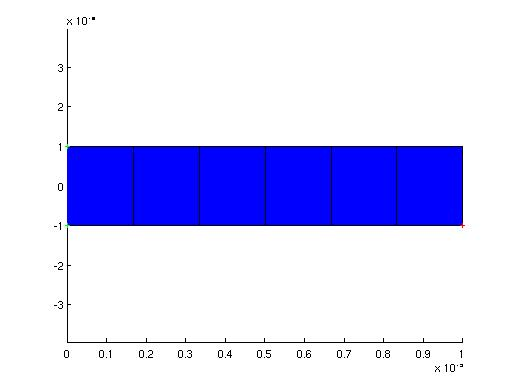
\includegraphics[height = 2in]{fig/mems_cant_m_mesh.jpg}
\caption{Mesh for a MEMS cantilever beam}
\label{fig:MEMSCantileverBeamMesh}
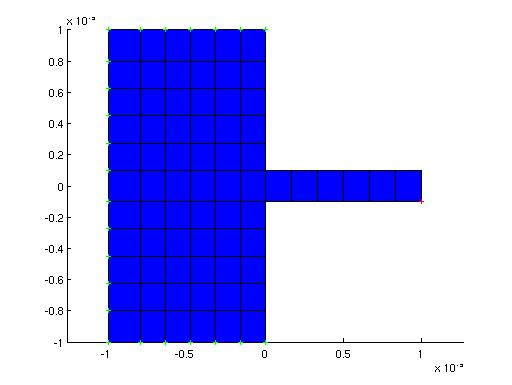
\includegraphics[height = 2in]{fig/mems_cant_wa_m_mesh.jpg}
\caption{Mesh for a MEMS cantilever beam with anchor}
\label{fig:MEMSCantileverBeamWaMesh}
\end{minipage}
\hfill
\begin{minipage}{0.45\linewidth}
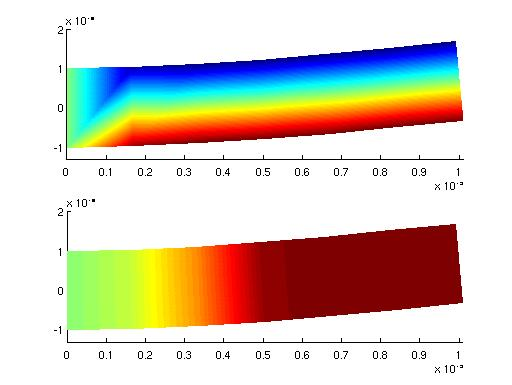
\includegraphics[height = 2in]{fig/mems_cant_m_sta.jpg}
\caption{Static deformation of a MEMS cantilever beam}
\label{fig:MEMSCantileverBeamStatic}
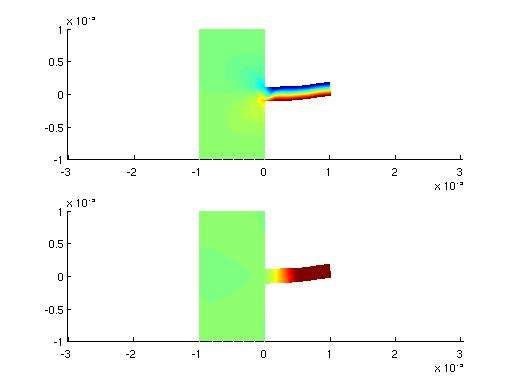
\includegraphics[height = 2in]{fig/mems_cant_wa_m_sta.jpg}
\caption{Static deformation of a MEMS cantilever beam with anchor}
\label{fig:MEMSCantileverBeamWaStatic}
\end{minipage}
\end{figure}



\clearpage
\subsubsection*{Solve dynamic modal problem (MATLAB)}
\begin{flushleft}
  \textbf{Inputfile:}
  \ttt{\ttilde/hiqlab/models/tutorial/mems\_cantilever\_beam/mems\_cant\_dyn.m}\\
\end{flushleft}
\hspace{1in}
{\footnotesize
\listinginput[10]{1}{../../../models/tutorial/mems_cantilever_beam/mems_cant_dyn.m}
}

\clearpage
The script conducts modal analysis and extracts the modes and 
frequencies of the beam.

\begin{itemize}

  \item{\textbf{Solve dynamic problem}}
  The variable \ttt{w0} defines the approximate value of the frequency 
  in radians that we are interested in. In this case we specify zero to 
  find those that are the smallest. \ttt{nev} eigenfrequencies are sought. 
  These are obtained by the function \ttt{mechmode}. The function returns 
  the mode shape, frequency[rad/s] and the $Q$. In this case, we have 
  not incorporated any damping and results will give us close to 
  infinite $Q$ values. For the case of anchor loss, a nonzero \ttt{w0}
  is given, since zero would not give the first bending mode as a result.

\end{itemize}

In the case where the nondimensionalized input file is used, nothing 
needs to be modified for the MATLAB script file which is used to solve 
the problem. The only thing that one must be aware of is which functions 
return dimensional quantaties from the mesh. This is noted in the section 
concerning non-dimensionalization.

The results obtained for the three input files are shown in 
Figures 
\ref{fig:MEMSCantileverBeamDynamic},
\ref{fig:MEMSCantileverBeamWaDynamic}.
The two figures show the mode obtained for the first bending mode
of the structure. 
Again, only one result is presented for the non-anchor case since
the dimensional and non-dimensional case return the same 
results. 

Though convergence of the solution is not obtained at this
mesh, the results are presented for reference.
\begin{verbatim}
No-anchor
------------------------------
Freq [Hz]   :3.101849e+07
            :2.181131e-07
Q           :7.110644e+13

Anchor
------------------------------
Freq [Hz]   :2.737977e+07
            :7.727477e+04
Q           :1.771592e+02
\end{verbatim}

\begin{figure}
\centering
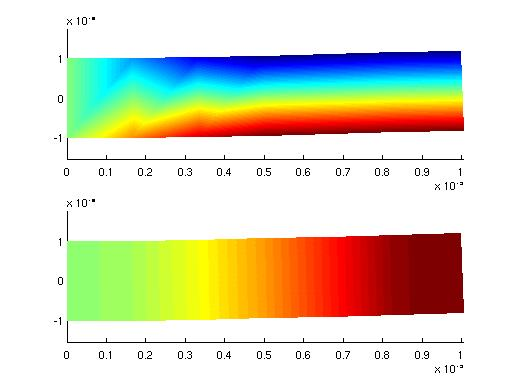
\includegraphics[height = 2in]{fig/mems_cant_m_dyn.jpg}
\caption{Dynamic mode of a MEMS cantilever beam}
\label{fig:MEMSCantileverBeamDynamic}
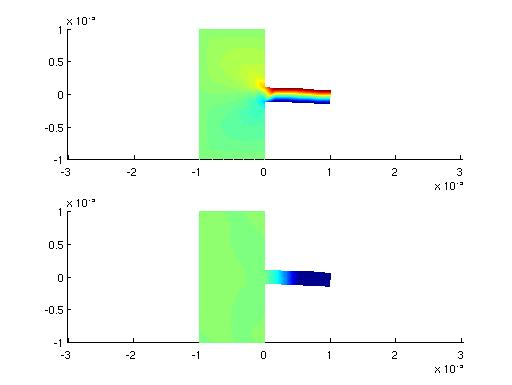
\includegraphics[height = 2in]{fig/mems_cant_wa_m_dyn.jpg}
\caption{Dynamic mode of a MEMS cantilever beam with anchor}
\label{fig:MEMSCantileverBeamWaDynamic}
\end{figure}


\clearpage
\subsubsection*{Solve for transfer function (MATLAB)}
\begin{flushleft}
  \textbf{Inputfile:}
  \ttt{\ttilde/hiqlab/models/tutorial/mems\_cantilever\_beam/mems\_cant\_tra.m}\\
\end{flushleft}
\hspace{1in}
{\footnotesize
\listinginput[10]{1}{../../../models/tutorial/mems_cantilever_beam/mems_cant_tra.m}
}

\clearpage
The script computes the transfer function between the force and 
displacement at the tip.

\begin{itemize}

  \item{\textbf{Compute forcing and sensing vectors}}
  The forcing and sensing vectors required for the transfer function 
  evaluation are obtained by the \ttt{Mesh\_get\_sense\_u} and 
  \ttt{Mesh\_get\_drive\_f} functions.

  \item{\textbf{Solve for transfer function}}
  \ttt{second\_order\_bode} is used to compute the transfer function.
  The range of the frequency that we would like to sweep across are 
  specified here. The variable \ttt{wc} defines the center frequency 
  of the sweep in [rad/s]. that we are interested in. The response and 
  frequency in [rad/s] are returned.

  \item{\textbf{Show bode plot}}
  The function \ttt{plot\_bode} is used to visualize the results.

\end{itemize}

In the case where the nondimensionalized input file is used, nothing 
needs to be modified for the MATLAB script file which is used to solve 
the problem. The only thing that one must be aware of is which functions 
return dimensional quantaties from the mesh. This is noted in the 
section concerning non-dimensionalization.

The results obtained for the three input files are shown in 
Figures 
\ref{fig:MEMSCantileverBeamTransfer},
\ref{fig:MEMSCantileverBeamWaTransfer}.
The two figures show the transfer function obtained for
the no-anchor and anchor case.
Again, only one result is presented for the non-anchor case since
the dimensional and non-dimensional case return the same 
results. 

Though convergence of the solution is not obtained at this
mesh, the results are presented for reference.

\begin{figure}
\centering
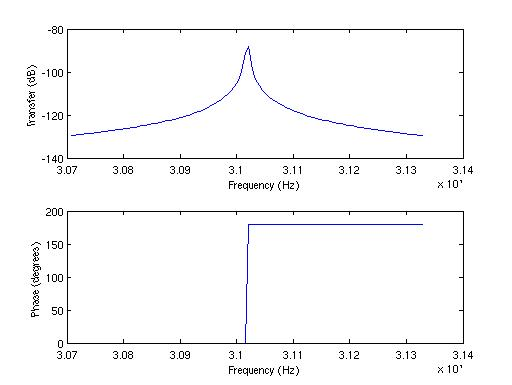
\includegraphics[height = 2in]{fig/mems_cant_m_tra.jpg}
\caption{Transfer function of a MEMS cantilever beam}
\label{fig:MEMSCantileverBeamTransfer}
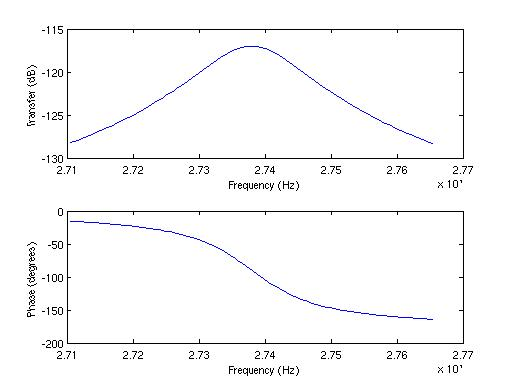
\includegraphics[height = 2in]{fig/mems_cant_wa_m_tra.jpg}
\caption{Transfer function of a MEMS cantilever beam with anchor}
\label{fig:MEMSCantileverBeamWaTransfer}
\end{figure}


\clearpage
\subsection{Thermomechanical analysis}
\begin{flushleft}
  \textbf{Inputfile:}
  \ttt{\ttilde/hiqlab/models/tutorial/mems\_cantilever\_beam}\\
  \textbf{Lua features introduced:}
  \ttt{ted\_nondim}\\
  \textbf{MATLAB features introduced:}
  \ttt{tedmode}
\end{flushleft}
This example is used to illustrate the analysis of the
thermo-mechanical response of a MEMS cantilever beam. For the coupled 
problem, the characteristic scales that govern the individual 
fields can vary greatly. Due to this fact, non-dimensionalization
should always be incorporated. For the thermoelastic case, this
can easily be done by defining the \ttt{ted\_nondim} function.

In this section, a differential temperature is applied to the
top and bottom of the beam to compute the static deflection
under this load. A schematic of this is shown in 
Figure~\ref{fig:MEMSCantileverBeam_Te_Sta}.
The modal analysis and transfer function response of this cantilever
beam in the configuration shown in 
Figure~\ref{fig:MEMSCantileverBeam_Mech} is also analyzed.

\begin{figure}[htbp]
\centering
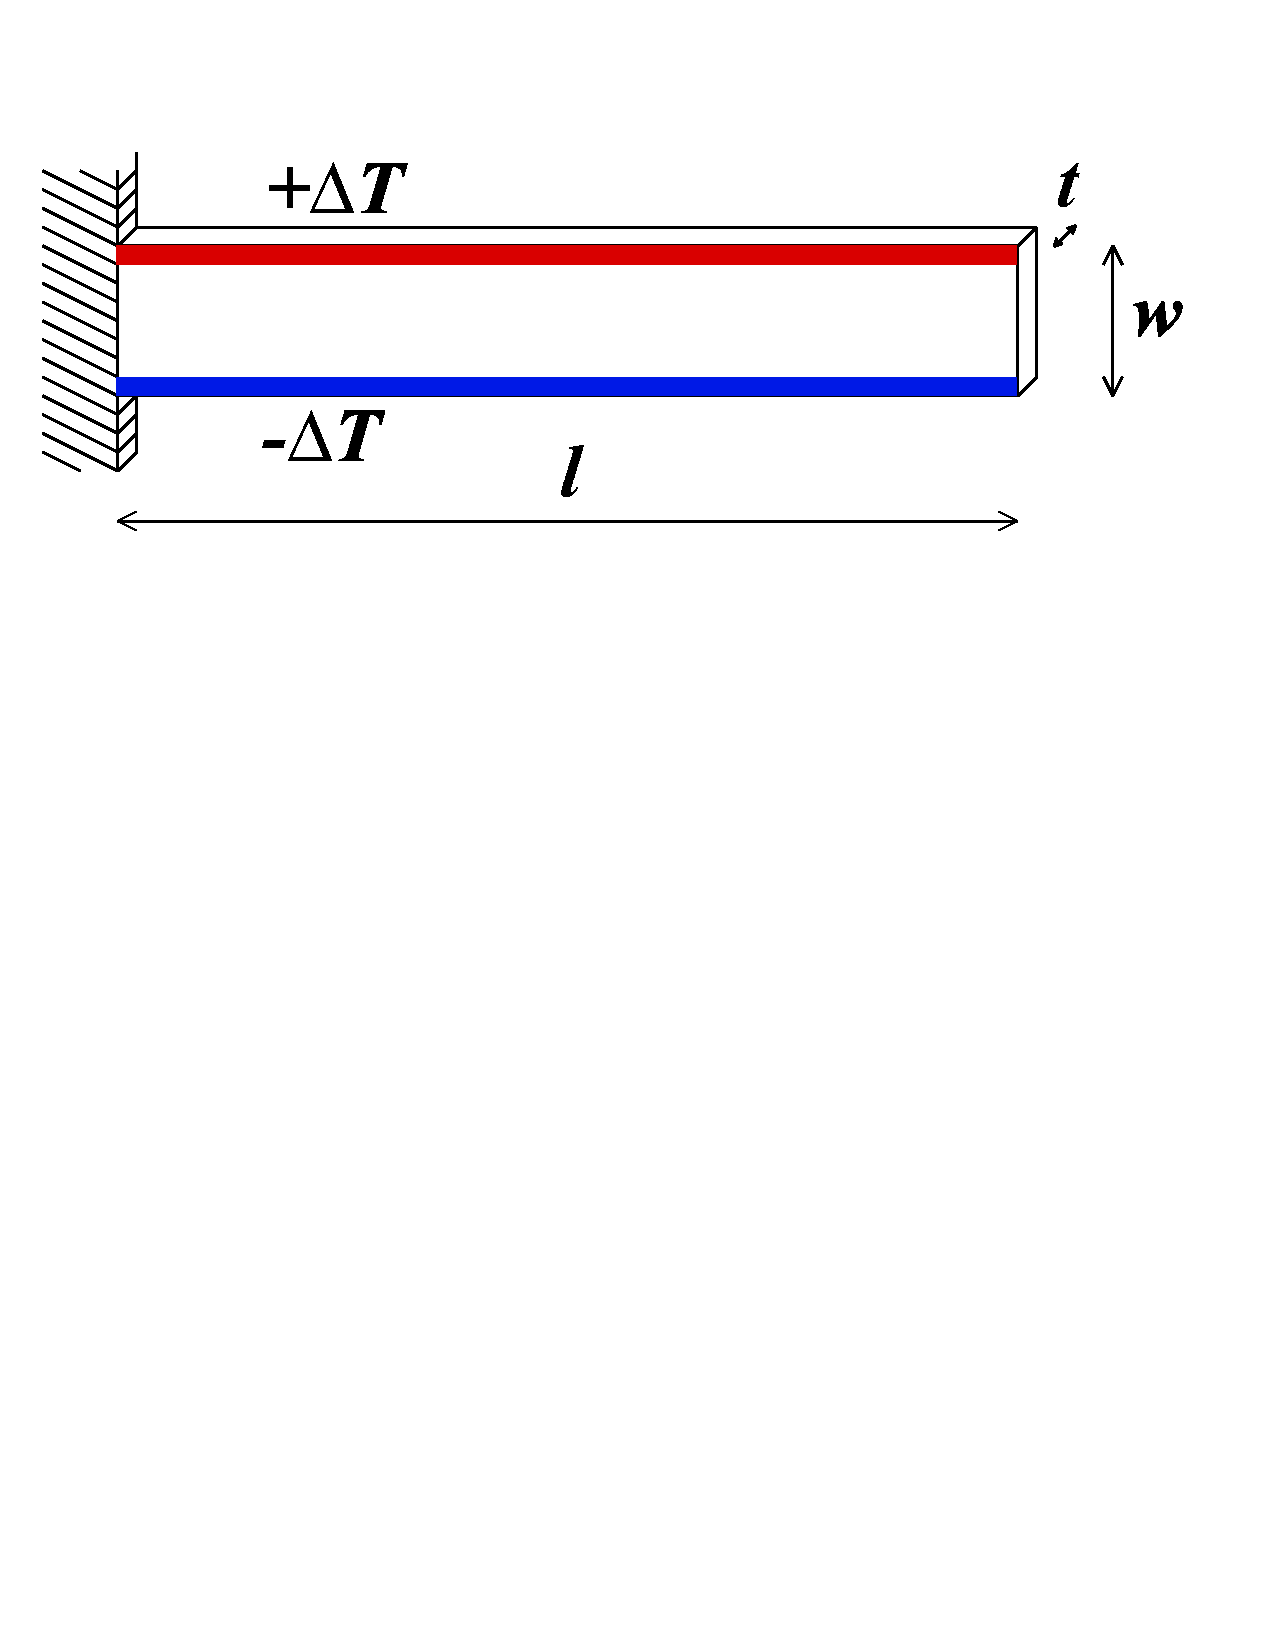
\includegraphics[trim = 0in 7in 0.5in 0in, clip, height = 2in]{fig/memscantileverbeam_te_sta.pdf}
\caption{Schematic of the MEMS cantilever beam (Thermoelastic static case)}
\label{fig:MEMSCantileverBeam_Te_Sta}
\end{figure}

\clearpage
\subsubsection*{Input file for static case (LUA)}
\begin{flushleft}
  \textbf{Inputfile:}
  \ttt{\ttilde/hiqlab/models/tutorial/mems\_cantilever\_beam/mems\_cant\_te\_sta.lua}\\
\end{flushleft}
\hspace{1in}
{\footnotesize
\listinginput[10]{1}{../../../models/tutorial/mems_cantilever_beam/mems_cant_te_sta.lua}
}

\clearpage
\begin{itemize}

  \item{\textbf{Define nondimensionalization parameters:}}
  Nondimensionalization is defined through the function \ttt{ted\_nondim}. 
  \begin{verbatim}
      -- Define nondimensionalization parameters
      ted_nondim('silicon2',7e-6)
  \end{verbatim}
  The first argument defines the material parameters used to define 
  the characteristic parameters; The second defines the characteristic 
  length scale.
  
  \item{\textbf{Define element type:}}
  For this analysis, a thermoelastic element is required. This can be 
  constructed by the function,
  \begin{verbatim}
      etype = make_material_te(mtype, 'planestress')
  \end{verbatim}

  \item{\textbf{Define boundary condition:}}
  For this case a constant temperature of 10 is applied to the top part 
  of the beam, and -10 to the bottom. The beam is fixed mechanically at 
  the left end.

\end{itemize}

\clearpage
\subsubsection*{Input file for dynamic modal and transfer function (LUA)}
\begin{flushleft}
  \textbf{Inputfile:}
  \ttt{\ttilde/hiqlab/models/tutorial/mems\_cantilever\_beam/mems\_cant\_te.lua}\\
\end{flushleft}
\hspace{1in}
{\footnotesize
\listinginput[10]{1}{../../../models/tutorial/mems_cantilever_beam/mems_cant_te.lua}
}

\clearpage
\subsubsection*{Solve static problem (MATLAB)}
Once the mesh is defined, the next step is to solve the problem.
Since this script is identical to the mechanical case we will only 
explain the parameters that are set.
\begin{itemize}

  \item{\textbf{Setting parameters:}}

\end{itemize}

\begin{figure}[htbp]
\begin{minipage}{0.45\linewidth}
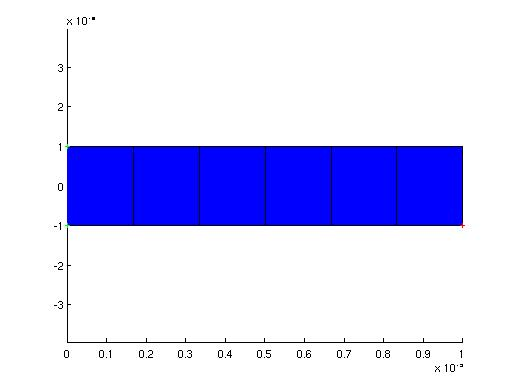
\includegraphics[height = 2in]{fig/mems_cant_m_mesh.jpg}
\caption{Mesh for a MEMS cantilever beam}
\label{fig:MEMSCantileverBeamTEMesh}
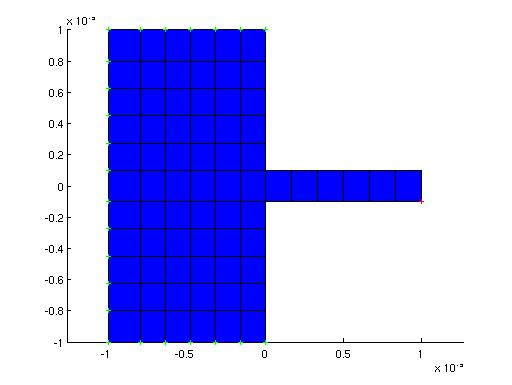
\includegraphics[height = 2in]{fig/mems_cant_wa_m_mesh.jpg}
\caption{Mesh for a MEMS cantilever beam with anchor}
\label{fig:MEMSCantileverBeamWaTEMesh}
\end{minipage}
\hfill
\begin{minipage}{0.45\linewidth}
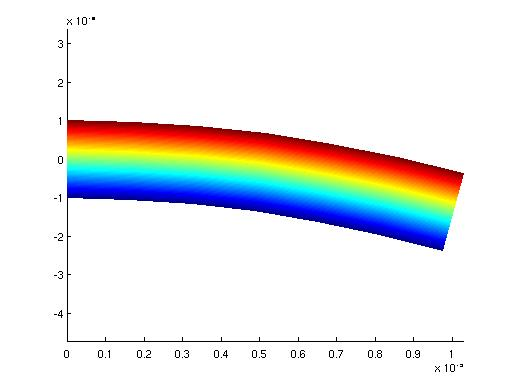
\includegraphics[height = 2in]{fig/mems_cant_te_sta.jpg}
\caption{Static deformation of a MEMS cantilever beam}
\label{fig:MEMSCantileverBeamTEStatic}
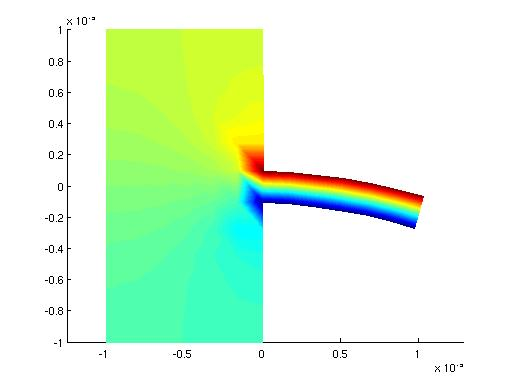
\includegraphics[height = 2in]{fig/mems_cant_wa_te_sta.jpg}
\caption{Static deformation of a MEMS cantilever beam with anchor}
\label{fig:MEMSCantileverBeamWaTEStatic}
\end{minipage}
\end{figure}

Results obtained were,
\begin{verbatim}
Tip displacement y:-1.359553e-09

Tip displacement y:-1.699258e-09
\end{verbatim}

\clearpage
\subsubsection*{Solve dynamic problem (MATLAB)}
Once the mesh is defined, the next step is to solve the problem.
Since this script is identical to the mechanical case we will only 
explain the parameters that are set.
\begin{itemize}

  \item{\textbf{Setting parameters:}}

\end{itemize}
Compared to the mechanical problem the value for \ttt{w0} is set to a
nonzero value. If \ttt{w0} were set to zero, there is a large possibility
that we would not obtain the mode of interest. By giving a close estimate
of the frequency of the mode of interest, the desired mode will be 
obtained with higher probability. This estimate \ttt{w0} may be obtained
from the purely mechanical analysis.

\begin{figure}
\centering
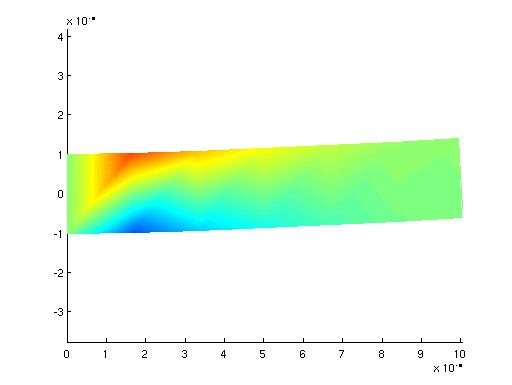
\includegraphics[height = 2in]{fig/mems_cant_te_dyn.jpg}
\caption{Dynamic mode of a MEMS cantilever beam}
\label{fig:MEMSCantileverBeamTEDynamic}
\includegraphics[height = 2in]{fig/mems_cant_wa_te_dyn.jpg}
\caption{Dynamic mode of a MEMS cantilever beam with anchor}
\label{fig:MEMSCantileverBeamWaTEDynamic}
\end{figure}

Results obtained were,
\begin{verbatim}
Freq [Hz]   :3.102175e+07
            :1.043208e+03
Q           :1.486844e+04

Freq [Hz]   :2.738287e+07
            :7.820706e+04
Q           :1.750672e+02
\end{verbatim}

\clearpage
\subsubsection*{Solve for transfer function  (MATLAB)}
Once the mesh is defined, the next step is to solve the problem.
Since this script is identical to the mechanical case we will only 
explain the parameters that are set.
\begin{itemize}

  \item{\textbf{Setting parameters:}}

\end{itemize}

\begin{figure}
\centering
\includegraphics[height = 2in]{fig/mems_cant_te_tra.jpg}
\caption{Transfer function of a MEMS cantilever beam}
\label{fig:MEMSCantileverBeamTETransfer}
\includegraphics[height = 2in]{fig/mems_cant_wa_te_tra.jpg}
\caption{Transfer function of a MEMS cantilever beam with anchor}
\label{fig:MEMSCantileverBeamWaTETransfer}
\end{figure}




\clearpage
\subsection{Electromechanical analysis}
\begin{flushleft}
  \textbf{Inputfile:}
  \ttt{\ttilde/hiqlab/models/tutorial/mems\_cantilever\_beam}\\
  \textbf{Lua functions used:}
\end{flushleft}
This example is used to illustrate the analysis of the
electro-mechanical response of a mems beam. For the coupled
problem, the characteristic scales that govern the individual
fields can vary greatly. Due to this fact, non-dimensionalization
should always be incorporated. For the electromechanical case, this
can easily be done by defining the \ttt{em\_nondim} function.

In this section, a voltage difference will be applied between the 
beam and the substrate. to compute the static deflection
under this load. Also, the dynamic response of this cantilever
beam, both the eigenvalues and transfer function response will
be evaluated. The model reduction technique for the electromechanical
problem will also be introduced.

\begin{figure}[htbp]
\centering
\includegraphics[trim = 0in 4in 0.5in 0in, clip, height = 2in]{fig/memscantileverbeam_em.pdf}
\caption{Schematic of the MEMS cantilever beam 
                              (Electromechanical static case)}
\label{fig:MEMSCantileverBeam_EM}
\end{figure}

\clearpage
\subsubsection*{Input file (LUA)}
\begin{flushleft}
  \textbf{Inputfile:}
  \ttt{\ttilde/hiqlab/models/tutorial/mems\_cantilever\_beam/mems\_cant\_em.lua}\\
\end{flushleft}
\hspace{1in}
{\footnotesize
\listinginput[10]{1}{../../../models/tutorial/mems_cantilever_beam/mems_cant_em.lua}
}

\clearpage
\begin{itemize}

  \item{\textbf{Define nondimensionalization parameters:}}
  Nondimensionalization is defined through the function \ttt{em\_nondim}.
  \begin{verbatim}
      -- Define nondimensionalization parameters
      em_nondim('silicon2',7e-6)
  \end{verbatim}
  The first argument defines the material parameters used to define 
  the characteristic parameters; The second defines the characteristic 
  length scale.

  \item{\textbf{Define element type:}}
  For this analysis, an electromechanical element is required besides 
  the elastic element. This can be constructed by the function,
  \begin{verbatim}
      etype = make_material_em(get_dim_scale('eps')*reps, 'planestress')
  \end{verbatim}
  By using the \ttt{get\_dim\_scale} function, the value of the 
  permitiviyt of free space can be extracted from the table 
  \ttt{dim\_scales}. 

  \item{\textbf{Define mesh using block command:}}
  Besides the mechanical beam, place electromechanical elements between 
  the underlying substrate and beam. Care must be taken in placing element 
  so that only one element is
  placed in this gap. Placing more than one element will introduce 
  hanging nodes.

  \item{\textbf{Define boundary condition:}}
  The beam is fixed mechanically at the left end. All mechanical 
  displacements within the gap are fixed to zero. A voltage of \ttt{V} 
  is applied to the beam and zero to the substrate through the 
  funtion \ttt{gap\_v\_bc}.

\end{itemize}

\clearpage
\subsubsection*{Solve static problem (MATLAB)}
Once the mesh is defined, the next step is to solve the problem.
Since this script is identical to the mechanical case we will only
explain the parameters that are set.
\begin{itemize}

  \item{\textbf{Setting parameters:}}

\end{itemize}
Since this electromechanical problem is nonlinear in the gap, 
a nonlinear iterative solve must be conducted. This is specified by 
the argument passed to the function \ttt{static\_state.m}.

Results obtained were,
\begin{verbatim}
Tip displacement y:-1.142867e-10
\end{verbatim}

\begin{figure}[htbp]
\centering
\includegraphics[height = 2in]{fig/mems_cant_em_mesh.jpg}
\caption{Mesh for a MEMS cantilever beam}
\label{fig:MEMSCantileverBeamEMMesh}
\includegraphics[height = 2in]{fig/mems_cant_em_sta.jpg}
\caption{Static deformation of a MEMS cantilever beam}
\label{fig:MEMSCantileverBeamEMStatic}
\end{figure}



\clearpage
\subsubsection*{Solve dynamic problem (MATLAB)}
Once the mesh is defined, the next step is to solve the problem.
Since this script is identical to the mechanical case we will only
explain the parameters that are set.
\begin{itemize}

  \item{\textbf{Setting parameters:}}

\end{itemize}
Compared to the mechanical problem the value for \ttt{w0} is set to a
nonzero value. If \ttt{w0} were set to zero, there is a large possibility
that we would not obtain the mode of interest. By giving a close estimate
of the frequency of the mode of interest, the desired mode will be
obtained with higher probability. This estimate \ttt{w0} may be obtained
from the purely mechanical analysis.

\begin{figure}
\centering
\includegraphics[height = 2in]{fig/mems_cant_em_dyn.jpg}
\caption{Dynamic mode of a MEMS cantilever beam}
\label{fig:MEMSCantileverBeamEMDynamic}
\end{figure}


\begin{verbatim}
Freq [Hz]   :2.791479e+07
            :3.452636e-11
Q           :4.042533e+17
\end{verbatim}

\clearpage
\subsubsection*{Solve for transfer function  (MATLAB)}
Once the mesh is defined, the next step is to solve the problem.
Since this script is identical to the mechanical case we will only
explain the parameters that are set.
\begin{itemize}

  \item{\textbf{Setting parameters:}}

\end{itemize}
The estimate for the center frequency should be obtained from the
previous dynamic eigenfrequency analysis. If model reduction is
required, only the value of \ttt{kmax} has to be set to a nonzero value.

\begin{figure}
\centering
\includegraphics[height = 2in]{fig/mems_cant_em_tra.jpg}
\caption{Transfer function of a MEMS cantilever beam}
\label{fig:MEMSCantileverBeamEMTransfer}
\end{figure}




\clearpage
\section{Device examples}
\subsection{An axisymmetric disk model}
\begin{flushleft}
  \textbf{Inputfile:}
  \ttt{\ttilde/hiqlab/models/developing/disk\_resonator/disk\_new}\\
  \textbf{Lua functions used:}
\end{flushleft}

\begin{figure}[htbp]
\centering
\includegraphics[trim = 0in 4in 0.1in 0in, clip, height = 3in]{fig/disk_resonator.pdf}
\caption{Schematic of the Disk resonator}
\label{fig:DiskResonator}
\end{figure}

\clearpage
\subsubsection*{Input file (LUA)}
\begin{flushleft}
  \textbf{Inputfile:}
  \ttt{\ttilde/hiqlab/models/developing/disk\_resonator/disk\_new/disk\_mesh.lua}\\
\end{flushleft}
\hspace{1in}
{\footnotesize
\listinginput[10]{1}{../../../models/developing/disk_resonator/disk_new/diskmesh.lua}
}

\clearpage
Only the portions emphasized are explained in detail.

\begin{itemize}

  \item{\textbf{Define element type:}}
  Two types of elastic material are defined, for modeling the 
  case where the post and disk material differ.

  \item{\textbf{Define driving and sensing functions:}}
  The disk is driven by a radial force at the perimeter and 
  sensed at the same location.

\end{itemize}

\clearpage
\subsubsection*{Solve dynamic modal problem (MATLAB)}
\begin{flushleft}
  \textbf{Inputfile:}
  \ttt{\ttilde/hiqlab/models/developing/disk\_resonator/disk\_new/disk\_dyn.m}\\
\end{flushleft}
\hspace{1in}
{\footnotesize
\listinginput[10]{1}{../../../models/developing/disk_resonator/disk_new/disk_dyn.m}
}

\clearpage
The steps to compute the dynamic modes of the disk resonator are 
explained here. 

\begin{itemize}

  \item{\textbf{Compute frequencies, Qs, and mode shapes:}}
  The function \ttt{mechmode} is used to compute \ttt{nev}
  modes closest to the frequence \ttt{w0}[rad/s]. The frequencies
  are sorted from proximity to \ttt{w0}.

  \item{\textbf{Show modes obtained:}}
  \ttt{plot\_mode} displays the obtained modes. Several options
  can be passed. In this case, the modes are animated by
  the \ttt{opt.animate} option which calls \ttt{plot\_cycle2d}. 

\end{itemize}

The modal values obtained for this problem are,
\begin{verbatim}
Freq [Hz]   :2.888937e+08
            :1.030763e+05
Q           :1.401359e+03
\end{verbatim}

\begin{figure}[htbp]
\centering
\includegraphics[height = 3in]{fig/disk_resonator_mesh.jpg}
\caption{Mesh of disk resonator}
\label{fig:DiskResonatorMesh}
\includegraphics[height = 3in]{fig/disk_resonator_mode.jpg}
\caption{Mode of disk resonator}
\label{fig:DiskResonatorMode}
\end{figure}

\clearpage
\subsubsection*{Solve for forced response (MATLAB)}
\begin{flushleft}
  \textbf{Inputfile:}
  \ttt{\ttilde/hiqlab/models/developing/disk\_resonator/disk\_new/disk\_for.m}\\
\end{flushleft}
\hspace{1in}
{\footnotesize
\listinginput[10]{1}{../../../models/developing/disk_resonator/disk_new/disk_for.m}
}

\clearpage
The steps to compute the dynamic response to a time harmonic
force of the disk resonator are explained here. 

\begin{itemize}

  \item{\textbf{Form driving pattern and obtain harmonic response:}}
  The driving pattern is obtained by \ttt{Mesh\_get\_drive\_f}
  which looks for the function \ttt{bode\_drive\_function} in 
  the Lua input file. Along with this driving pattern the 
  forcing frequency \ttt{w}[rad/s] is given to the 
  \ttt{harmonic\_state}.

\end{itemize}

\clearpage
\subsubsection*{Solve for transfer function (MATLAB)}
\begin{flushleft}
  \textbf{Inputfile:}
  \ttt{\ttilde/hiqlab/models/developing/disk\_resonator/disk\_new/disk\_tra.m}\\
\end{flushleft}
\hspace{1in}
{\footnotesize
\listinginput[10]{1}{../../../models/developing/disk_resonator/disk_new/disk_tra.m}
}

\clearpage
The steps to compute the transfer function of the disk 
resonator are explained here. 

\begin{itemize}

  \item{\textbf{Form driving and sensing pattern:}}
  These are obtained by calling the functions 
  \ttt{Mesh\_get\_drive\_f} and \ttt{Mesh\_get\_sense\_u}
  which in turn look for the functions 
  \ttt{bode\_drive\_function} and \ttt{bode\_sense\_function}
  in the Lua input file.

  \item{\textbf{Computing transfer function:}}
  \ttt{second\_order\_bode} computes the transfer function
  of a second order system. The transfer function in the
  range of [\ttt{wr\_min*wc},\ttt{wr\_max*wc}] with \ttt{w\_ndiv}
  data points is computed. Optionally, a reduced order model (ROM) 
  can be formed to speed the computation. This is done by 
  specifying the \ttt{kmax} option which defines the size
  of the ROM. In the PML case, a real basis
  can be selected for projection by the option \ttt{realbasis}.
  This option will double the size of the ROM.
 
  \item{\textbf{Show bode plot:}}
  The option \ttt{visualQ} computes and displays the Q value 
  computed from the data points. Enough data points are requred
  for an accurate value.  

\end{itemize}

\begin{figure}[htbp]
\centering
\includegraphics[height = 3in]{fig/disk_resonator_forced.jpg}
\caption{Forced response of disk resonator}
\label{fig:DiskResonatorForced}
\includegraphics[height = 3in]{fig/disk_resonator_transfer.jpg}
\caption{Transfer function  of disk resonator}
\label{fig:DiskResonatorTransfer}
\end{figure}

\clearpage
\subsection{Michigan Free-Free beam}
\begin{flushleft}
  \textbf{Inputfile:}
  \ttt{\ttilde/hiqlab/models/developing/mich\_la\_fr\_beam}\\
  \textbf{Lua functions used:}
\end{flushleft}

\begin{figure}[htbp]
\centering
\includegraphics[trim = 0in 4in 1in 0in, clip, height = 3in]{fig/mich_la_frfr_beam2d_small.pdf}
\caption{Schematic of the Michigan Beam Resonator}
\label{fig:MichiganBeamResonator}
\end{figure}

\clearpage
\subsubsection*{Input file (LUA)}
\begin{flushleft}
  \textbf{Inputfile:}
  \ttt{\ttilde/hiqlab/models/developing/mich\_la\_fr\_beam/2d/mich\_la\_frfr\_beam2d.lua}\\
\end{flushleft}
\hspace{1in}
{\footnotesize
\listinginput[10]{1}{../../../models/developing/mich_la_fr_beam/2d/mich_la_frfr_beam2d.lua}
}

\clearpage
Only the portions emphasized are explained in detail.

\begin{itemize}

  \item{\textbf{Including function definition file:}}
  When the mesh generation of a particular geometry becomes
  complex, it is often useful to construct a seperate Lua
  file and include this by calling \ttt{require}. In this
  case \ttt{generate\_frfr\_beam2d.lua} is called.

  \item{\textbf{Define nondimensionalization parameters:}}
  The material \ttt{silicon2} and the length scale of 
  \ttt{2d-6} are used to define the characteristic parameters
  for the thermoelastic analysis through the function 
  \ttt{ted\_nondim}.

  \item{\textbf{Generate Free-Free beam:}}
  The function \ttt{generate\_frfr\_beam2d} is called from
  the file \ttt{generate\_frfr\_beam2d.lua}. The input
  arguments define the location and angle of rotation of the
  device in global coordinates. The function returns a table 
  of functions which define the boundary condition and stretch
  functions of the anchor.  

\end{itemize}

\clearpage
\subsubsection*{Solve dynamic modal problem (MATLAB)}
\begin{flushleft}
  \textbf{Inputfile:}
  \ttt{\ttilde/hiqlab/models/developing/mich\_la\_fr\_beam/2d/mich\_la\_frfr\_beam2d\_dyn.m}\\
\end{flushleft}
\hspace{1in}
{\footnotesize
\listinginput[10]{1}{../../../models/developing/mich_la_fr_beam/2d/mich_la_frfr_beam2d_dyn.m}
}

\clearpage
The steps to compute the dynamic modes of the disk resonator are 
explained here. 

\begin{itemize}

  \item{\textbf{Compute frequencies, Qs, and mode shapes:}}
  The function \ttt{tedmode} is used to compute \ttt{nev}
  modes closest to the frequence \ttt{w0}[rad/s]. 

  \item{\textbf{Show modes obtained:}}
  \ttt{plot\_mode} displays the obtained modes. Several options
  can be passed. In this case, the modes are animated by
  the \ttt{opt.animate} option which calls \ttt{plot\_cycle2d}. 
  Also \ttt{cfields} is specified to show the thermal fluctuations
  for the color field.

\end{itemize}

The modal values obtained are,
\begin{verbatim}
Freq [Hz]   :9.592613e+06
            :3.572215e+02
Q           :1.342670e+04
\end{verbatim}

\begin{figure}[htbp]
\centering
\includegraphics[height = 3in]{fig/mich_resonator_mesh.jpg}
\caption{Mesh of the beam resonator}
\label{fig:MichResonatorMesh}
\includegraphics[height = 3in]{fig/mich_resonator_mode.jpg}
\caption{Mode of the beam resonator}
\label{fig:MichResonatorMode}
\end{figure}

\clearpage
\subsubsection*{Solve dynamic forced problem (MATLAB)}
\begin{flushleft}
  \textbf{Inputfile:}
  \ttt{\ttilde/hiqlab/models/developing/mich\_la\_fr\_beam/2d/mich\_la\_frfr\_beam2d\_for.m}\\
\end{flushleft}
\hspace{1in}
{\footnotesize
\listinginput[10]{1}{../../../models/developing/mich_la_fr_beam/2d/mich_la_frfr_beam2d_for.m}
}

\clearpage
The steps to compute the dynamic response to a time harmonic
force of the beam resonator are explained here. 

\begin{itemize}

  \item{\textbf{Form driving pattern and obtain harmonic response:}}
  The driving pattern is obtained by \ttt{Mesh\_get\_drive\_f}
  which looks for the function \ttt{bode\_drive\_function} in 
  the Lua input file. Along with this driving pattern the 
  forcing frequency \ttt{w}[rad/s] is given to the 
  \ttt{harmonic\_state}. The option \ttt{mkc} is set to one
  specifying that the damping term \ttt{C} be included in the 
  computation. This must be specified for the thermoelastic 
  case. 

\end{itemize}

\clearpage
\subsubsection*{Solve transfer function problem (MATLAB)}
\begin{flushleft}
  \textbf{Inputfile:}
  \ttt{\ttilde/hiqlab/models/developing/mich\_la\_fr\_beam/2d/mich\_la\_frfr\_beam2d\_tra.m}\\
\end{flushleft}
\hspace{1in}
{\footnotesize
\listinginput[10]{1}{../../../models/developing/mich_la_fr_beam/2d/mich_la_frfr_beam2d_tra.m}
}

\clearpage
The steps to compute the transfer function of the disk
resonator are explained here. 

\begin{itemize}

  \item{\textbf{Form driving and sensing pattern:}}
  These are obtained by calling the functions
  \ttt{Mesh\_get\_drive\_f} and \ttt{Mesh\_get\_sense\_u}
  which in turn look for the functions
  \ttt{bode\_drive\_function} and \ttt{bode\_sense\_function}
  in the Lua input file.

  \item{\textbf{Computing transfer function:}}
  \ttt{second\_order\_bode} computes the transfer function
  of a second order system. The transfer function in the
  range of [\ttt{wr\_min*wc},\ttt{wr\_max*wc}] with \ttt{w\_ndiv}
  data points is computed. The option \ttt{mkc} is set to one
  specifying that the damping term \ttt{C} be included in the 
  computation. This must be specified for the thermoelastic 
  case. Optionally, a reduced order model (ROM)
  can be formed to speed the computation. This is done by
  specifying the \ttt{kmax} option which defines the size
  of the ROM. In the PML case, a real basis
  can be selected for projection by the option \ttt{realbasis}.
  This option will double the size of the ROM. For the 
  thermoelastic case an additional strucutre preseravation
  basis can be selected by \ttt{structurep}. To do this
  the function \ttt{ted\_block\_mesh} which reorders the 
  \ttt{id} array into mechanical and thermal must be called
  after \ttt{Mesh\_load} as is done in this example.
  This option will double the size of the ROM. 

\end{itemize}

\begin{figure}[htbp]
\centering
\includegraphics[height = 3in]{fig/mich_resonator_forced.jpg}
\caption{Forced response of Michigan resonator}
\label{fig:MichResonatorForced}
\includegraphics[height = 3in]{fig/mich_resonator_transfer.jpg}
\caption{Transfer function  of Michigan resonator}
\label{fig:MichResonatorTransfer}
\end{figure}

\clearpage
\subsection{Circuit test}
\subsubsection{Low pass filter}
\begin{flushleft}
  \textbf{Inputfile:}
  \ttt{\ttilde/hiqlab/models/tutorial/circuit\_test}\\
  \textbf{Lua functions used:}
\end{flushleft}

\begin{figure}[htbp]
\centering
\includegraphics[trim = 0in 5in 1in 1in, clip, height = 3in]{fig/lowpassfilter.pdf}
\caption{Schematic of the Low pass filter}
\label{fig:LowPassFilter}
\end{figure}

\clearpage
\subsubsection*{Input file (LUA)}
\begin{flushleft}
  \textbf{Inputfile:}
  \ttt{\ttilde/hiqlab/models/tutorial/circuit\_test/low\_pass\_filter.lua}\\
\end{flushleft}
\hspace{1in}
{\footnotesize
\listinginput[10]{1}{../../../models/tutorial/circuit_test/low_pass_filter.lua}
}

\clearpage
Only the portions emphasized are explained in detail.

\begin{itemize}

  \item{\textbf{Construct element:}}
  \ttt{make\_material\_LRC} constructs the lumped LRC component
  models used in circuit analysis. The first argument specifies
  the value of the element, and the second the type of component.
  \ttt{make\_material\_wire} constructs an element which 
  can be used for a short circuited wire and additionaly 
  voltage or current sources depending on the element variable 
  boundary conditions that are set.

  \item{\textbf{Add elements to mesh:}}
  The lumped LRC elements are connected between two nodes
  with appropriate node numbers. Since we would like to specify
  a voltage source on the \ttt{wire} element through an element
  variable boundary condition, the element number \ttt{elem1}
  must be extracted and stored for reference.

  \item{\textbf{Define nodal boundary condition:}}
  The nodes which are grounded are specified.

  \item{\textbf{Define driving and sensing functions:}}
  The circuit is driven with an AC voltage source defined 
  through an element variable driving condition on the 
  \ttt{wire} element by the function \ttt{ac\_voltage\_source}. 
  If the index of the
  element \ttt{ind} equals the element number \ttt{elem1} of
  the wire, a value of \ttt{E} is specfied as the voltage
  difference between the nodes that \ttt{wire} is connected to. 

  The voltages at node 3 an 4 are sensed. 

\end{itemize}

\clearpage
\subsubsection*{Solve for transfer function (MATLAB)}
\begin{flushleft}
  \textbf{Inputfile:}
  \ttt{\ttilde/hiqlab/models/tutorial/circuit\_test/low\_pass\_filter.m}\\
\end{flushleft}
\hspace{1in}
{\footnotesize
\listinginput[10]{1}{../../../models/tutorial/circuit_test/low_pass_filter.m}
}

\clearpage
The steps to compute the transfer function of the low pass
filter are explained here. 

\begin{itemize}

  \item{\textbf{Get driving and sensing patterns:}}
  The sensing patterns for the voltages at node 3 and 4
  are obtained by the function \ttt{Mesh\_get\_sense\_u}
  which in turn look for the appropriate functions in the
  Lua input file. Since the driving pattern is obtained
  by the contribution that comes from an element variable
  in \ttt{wire} defined by the Lua function 
  \ttt{ac\_voltage\_source}, it must be called by 
  \ttt{Mesh\_get\_drive\_elements\_f}.

  \item{\textbf{Compute transfer function:}}
  The frequency range can also be set in a logarthmic
  spacing by the option \ttt{w\_type}. In this case
  the range is set as [\ttt{10\^(-2)*wc,10\^(3)*wc}]
  with \ttt{w\_ndiv} divisions. Though this is a first
  order problem the function second order bode can be 
  called for transfer function evaluation, but the 
  option  \ttt{mkc} must be set to 1 to include the 
  \ttt{C} matrix.

\end{itemize}

\begin{figure}[htbp]
\centering
\includegraphics[height = 3in]{fig/low_pass_filter_mesh.jpg}
\caption{Mesh for a Low pass filter}
\label{fig:LowPassFilterMesh}
\includegraphics[height = 3in]{fig/low_pass_filter_transfer.jpg}
\caption{Transfer function  for a Low pass filter}
\label{fig:LowPassFilterTransfer}
\end{figure}

\clearpage
\subsubsection{Ladder filter}
\begin{flushleft}
  \textbf{Inputfile:}
  \ttt{\ttilde/hiqlab/models/developing/circuit\_test}\\
  \textbf{Lua functions used:}
\end{flushleft}

\begin{figure}[htbp]
\centering
\includegraphics[trim = 0in 5in 0in 0in, clip, height = 3in]{fig/ladderfilter.pdf}
\caption{Schematic of the Ladder filter}
\label{fig:LadderFilter}
\end{figure}

\clearpage
\subsubsection*{Input file (LUA)}
\begin{flushleft}
  \textbf{Inputfile:}
  \ttt{\ttilde/hiqlab/models/tutorial/circuit\_test/ladder\_filter.lua}\\
\end{flushleft}
\hspace{1in}
{\footnotesize
\listinginput[10]{1}{../../../models/tutorial/circuit_test/ladder_filter.lua}
}

\clearpage
Only the portions emphasized are explained in detail.

\begin{itemize}

  \item{\textbf{Define circuit elements:}}
  The flags \ttt{insert1} and \ttt{insert2} allow 
  one to select which filters are included in the circuit.
  The material properties of the lumped LRC components can
  also be complex, in which case a table with the real and
  imaginary parts are passed to the \ttt{make\_material\_LRC}
  constructor. The element number of the \ttt{wire} added between
  nodes 1 and 2 have been returned since an element variable driving 
  condition will be added for the ac voltage source.

  \item{\textbf{Define nodal boundary condition:}}
  The nodes which are grounded are specified.

  \item{\textbf{Define driving and sensing functions:}}
  The circuit is driven with an AC voltage source defined 
  through an element variable driving condition on the 
  \ttt{wire} element by the function \ttt{ac\_voltage\_source}. 
  If the index of the
  element \ttt{ind} equals the element number \ttt{elem1} of
  the wire, a value of \ttt{E} is specfied as the voltage
  difference between the nodes that \ttt{wire} is connected to. 

  The voltages at node 3 an 17 are sensed. 

\end{itemize}

\clearpage
\subsubsection*{Solve for transfer function (MATLAB)}
\begin{flushleft}
  \textbf{Inputfile:}
  \ttt{\ttilde/hiqlab/models/tutorial/circuit\_test/ladder\_filter.m}\\
\end{flushleft}
\hspace{1in}
{\footnotesize
\listinginput[10]{1}{../../../models/tutorial/circuit_test/ladder_filter.m}
}

\clearpage
The steps to compute the transfer function of the low pass
filter are explained here. 

\begin{itemize}

  \item{\textbf{Get driving and sensing patterns:}}
  The sensing patterns for the voltages at node 3 and 4
  are obtained by the function \ttt{Mesh\_get\_sense\_u}
  which in turn look for the appropriate functions in the
  Lua input file. Since the driving pattern is obtained
  by the contribution that comes from an element variable
  in \ttt{wire} defined by the Lua function
  \ttt{ac\_voltage\_source}, it must be called by
  \ttt{Mesh\_get\_drive\_elements\_f}.

  \item{\textbf{Compute transfer function:}}
  Though this is a first
  order problem the function second order bode can be
  called for transfer function evaluation, but the
  option  \ttt{mkc} must be set to 1 to include the
  \ttt{C} matrix.

  \item{\textbf{Compute analytical result:}}
  For this case the analytical result is computed.

\end{itemize}

\begin{figure}[htbp]
\centering
\includegraphics[height = 3in]{fig/ladder_filter_mesh.jpg}
\caption{Mesh for a Ladder filter}
\label{fig:LadderFilterMesh}
\includegraphics[height = 3in]{fig/ladder_filter_transfer.jpg}
\caption{Transfer function  for a Ladder filter}
\label{fig:LadderFilterTransfer}
\end{figure}

\clearpage
\subsection{Electrostatic parallel plate capacitor}
\begin{flushleft}
  \textbf{Inputfile:}
  \ttt{\ttilde/hiqlab/models/tutorial/e\_pp\_capacitor}\\
  \textbf{Lua functions used:}
\end{flushleft}

\begin{figure}[htbp]
\begin{minipage}{0.3\linewidth}
\includegraphics[trim = 1in 4.5in 2in 0.5in, clip, height = 2.5in]{fig/e_capacitor_fix.pdf}
\caption{Capacitor with fixed boundary conditions on potentials}
\end{minipage}
\hfill
\begin{minipage}{0.3\linewidth}
\includegraphics[trim = 1in 4.5in 2in 0.5in, clip, height = 2.5in]{fig/e_capacitor_globals.pdf}
\caption{Capacitor with potentials fixed to global variables}
\end{minipage}
\hfill
\begin{minipage}{0.3\linewidth}
\includegraphics[trim = 1in 4.5in 2in 0.5in, clip, height = 2.5in]{fig/e_capacitor_electrodes.pdf}
\caption{Capacitor with potentials fixed to nodal volatage}
\end{minipage}
\end{figure}

\clearpage
\subsubsection*{Input file (LUA)}
\begin{flushleft}
  \textbf{Inputfile:}
  \ttt{\ttilde/hiqlab/models/tutorial/e\_pp\_capacitor/e\_pp\_capacitor2d.lua}\\
\end{flushleft}
\hspace{1in}
{\footnotesize
\listinginput[10]{1}{../../../models/tutorial/e_pp_capacitor/e_pp_capacitor2d.lua}
}

\clearpage
Only the portions emphasized are explained in detail.

\begin{itemize}

  \item{\textbf{Define element type:}}
  Constuct an electrostatic element with the constructor
  \ttt{make\_material\_electrostatic} where the first 
  argument specifies the permitivity of the element.

  \item{\textbf{Set boundary condition:}}
  If no string is set to \ttt{use\_case} then
  nodal boundary conditions are set to the top and bottom
  potential variables. 

  If \ttt{use\_case=='eppc2d\_using\_globals\_sta.lua'}, then
  the file \ttt{eppc2d\_using\_globals\_sta.lua} is loaded.
  The file is shown in Figure 
  \ref{fig:LuaInputFile:eppc2d_using_globals_sta.lua}.
  \begin{itemize}

     \item{\textbf{Define global shape functions:}}
     Two global shape functions are defined for the two global
     variables.

     \item{\textbf{Add global variables:}}
     The two global variables are added by the \ttt{mesh:add\_global} 
     command. The first argument specifies the function associated with 
     the global variable. The second and third arguments are 
     the values that are used to non-dimensionalize the primary
     and secondary variable. Since we would like to define
     boundary conditions on these global variables, the number of
     the global variable must be stored in \ttt{idg\_t,idg\_b}. 

     \item{\textbf{Define global variable boundary condtion function:}}
     A function with the global variable number as the input 
     argument is defined to specify global variable boundary 
     conditions. When the number \ttt{idg} is equal to the 
     \ttt{idg\_t}, the global variable number associated with the top
     electrode, a value of \ttt{Vf\_dc} is assigned. 
     When the number \ttt{idg} is equal to the 
     \ttt{idg\_b}, the global variable number associated with the 
     bottom electrode, a value of zero is assigned. 

     \item{\textbf{Set global variables:}}
     Once the global variables are added to the mesh they must
     be set by the \ttt{mesh:set\_globals()} command. 

     \item{\textbf{Set global variable boundary conditions:}}
     The global variable boundary condition is set by the command
     \ttt{mesh:set\_globals\_bc}.

  \end{itemize}

  If \ttt{use\_case=='eppc2d\_using\_electrodes\_sta.lua'}, then
  the file \ttt{eppc2d\_using\_electrodes\_sta.lua} is loaded.
  The file is shown in Figure 
  \ref{fig:LuaInputFile:eppc2d_using_electrodes_sta.lua}.
  \begin{itemize}

     \item{\textbf{Add nodes:}}
     To use the electrode element they must connected to nodes 
     with voltage variables. These nodes are added in these lines
     of code.

     \item{\textbf{Define global shape functions:}}
     Two global shape functions are defined for the two global
     variables that are incorporated in the electrode element.

     \item{\textbf{Add electrode element:}}
     The electrode element is added by the function
     \ttt{add\_electrode}. The first argument specifies the 
     type of electrode used. The second argument specifies the 
     number of node that the electrode is connected to. The
     third specifies the global variable shape function that
     is used to tie the potential variables to the voltage variable
     of the node. The last argument is an optional scaling parameter
     to account for the 2D analysis.(See section on electrode for
     details). This constructor can return the element number of 
     the electrode element (\ttt{eno\_d,eno\_s}) and the global 
     variable number of the global variable (\ttt{idg\_d,idg\_s}). 
     These should be stored for reference, since they are requred
     for modal computation and equivalent circuit parameter 
     extraction. 

     \item{\textbf{Define nodal boundary condition:}}
     One node is specified to have voltage of \ttt{Vf\_dc}
     and the other is zero. The boundary condition for the 
     voltages are specified in the second slot since the 
     first slot is specified for the potential variables. These
     are distinguished since the dual variable for potentials 
     are defined as the charge, and the dual variable for the
     voltages are the currents. Since elements connecting 
     potential variables were added first the potentials are
     specified in the first slot.   

     \item{\textbf{Element variable sensing functions:}}
     For the electrode element, the global variable pertains
     to the element and can be accessed also as an element 
     variable. For the electrode element the first element 
     variable accesses this global variable which is the 
     voltage. The second element variable is the total charge.

     These can are sensed by the functions defined here.

     \item{\textbf{Set global variables:}}
     Once the global variables are added to the mesh they must
     be set by the \ttt{mesh:set\_globals()} command. 

     \item{\textbf{Set global variable boundary conditions:}}
     The global variable boundary condition is set by the command
     \ttt{mesh:set\_globals\_bc}.

  \end{itemize}

  \item{\textbf{Nodal variable sensing functions:}}
  The function \ttt{sense\_top\_Q} is used to sense the potentials
  on the top electrode and \ttt{sense\_bot\_Q} for the bottom.
 
\end{itemize}

\clearpage
\begin{figure}[htbp]
  {\footnotesize
  \listinginput[10]{1}{../../../models/tutorial/e_pp_capacitor/eppc2d_using_globals_sta.lua}
  }
  \caption{Lua input file for an electrostatic parallel plate
   capacitor using globals (\ttt{eppc2d\_using\_globals\_sta.lua})}
  \label{fig:LuaInputFile:eppc2d_using_globals_sta.lua}
\end{figure}

\begin{figure}[htbp]
  {\footnotesize
  \listinginput[10]{1}{../../../models/tutorial/e_pp_capacitor/eppc2d_using_electrodes_sta.lua}
  }
  \caption{Lua input file for an electrostatic parallel plate
capacitor using electrodes (\ttt{eppc2d\_using\_electrodes\_sta.lua})}
  \label{fig:LuaInputFile:eppc2d_using_electrodes_sta.lua}
\end{figure}

\clearpage
\subsubsection*{Solve electrostatic problem (MATLAB)}
\begin{flushleft}
  \textbf{Inputfile:}
  \ttt{\ttilde/hiqlab/models/tutorial/e\_pp\_capacitor/e\_pp\_capacitor2d\_sta.m}\\
\end{flushleft}
\hspace{1in}
{\footnotesize
\listinginput[10]{1}{../../../models/tutorial/e_pp_capacitor/e_pp_capacitor2d_sta.m}
}

\clearpage
The steps to compute the static state of an electrostatic 
parallel plate capacitor are 
explained here. 

\begin{itemize}

  \item{\textbf{Parameters:}}
  Select which case to use.

  \item{\textbf{Analytical solution:}}
  Extract numerical parameters from the Lua environment through the 
  function \ttt{Lua\_get\_double}, and compute the capacitance
  from the formula for a parallel plate capacitor.

  \item{\textbf{Find top and bottom charge from sensing nodal values:}}
  \ttt{Mesh\_get\_force} extracts the forces that result at the 
  nodal degrees of freedom. \ttt{force1} is a \ttt{ndf}-by-\ttt{numnp}
  array. In this case \ttt{ndf} is 1 or 2 if you use the electrode 
  element. \ttt{Mesh\_get\_sense\_force} returns the sensing vector
  for the Lua function in the \ttt{ndf}-by-\ttt{numnp} format. 
  These are contracted to obtain the charge. This charge is in
  units of Coulomb's per unit normalized length due to the plane
  assumption. Thus if we assume that the capacitor has a \ttt{Ct}
  thickness in the $z$ direction, the charge must be multiplied
  by \ttt{Ct}/\ttt{cL}, which is done to compute the capacitance.
  The normalized scale for length is obtained from the mesh through
  \ttt{Mesh\_get\_scale}.

  \item{\textbf{Find top and bottom charge from sensing free dofs:}}
  In the case that electrods are present, the total charge on the
  top and bottom of the electrode can be obtained through the 
  element variable. These are sensed by the call to 
  \ttt{Mesh\_get\_sense\_elements\_u}. Contracting this sense vector
  with the noramlized displacement vector yields the charge in 
  dimensional form. This charge is in
  units of Coulomb's per unit normalized length due to the plane
  assumption. Thus if we assume that the capacitor has a \ttt{Ct}
  thickness in the $z$ direction, the charge must be multiplied
  by \ttt{Ct}/\ttt{cL}, which is done to compute the capacitance.
  The normalized scale for length is obtained from the mesh through
  \ttt{Mesh\_get\_scale}.

\end{itemize}

Computed values for capacitance are,
\begin{verbatim}
Analytic capacitance:1.062503e-14
Computed capacitance:1.062503e-14
\end{verbatim}


\begin{figure}[htbp]
\centering
\includegraphics[height = 2in]{fig/e_pp_capacitor_mesh_fix.jpg}
\caption{Mesh for a Parallel plate capacitor using fixed boundary conditions
         on potentials or global variables}
\label{fig:ElectrostaticParallelPlateCapacitorFixMesh}
\includegraphics[height = 2in]{fig/e_pp_capacitor_mesh_electrodes.jpg}
\caption{Mesh for a Parallel plate capacitor using electrodes}
\label{fig:ElectrostaticParallelPlateCapacitorElectrodesMesh}
\includegraphics[height = 2in]{fig/e_pp_capacitor_field.jpg}
\caption{Potential field for a Parallel plate capacitor}
\label{fig:ElectrostaticParallelPlateCapacitorPotentialField}
\end{figure}

\clearpage
\subsection{Electromechanical parallel plate capacitor}
\begin{flushleft}
  \textbf{Inputfile:}
  \ttt{\ttilde/hiqlab/models/developing/em\_pp\_capacitor}\\
  \textbf{Lua functions used:}
\end{flushleft}

\begin{figure}[htbp]
\centering
\includegraphics[trim = 1in 3.5in 2in 0.5in, clip, height = 2.5in]{fig/em_capacitor.pdf}
\caption{Electromechanical Capacitor}
\end{figure}

\clearpage
\subsubsection*{Input file (LUA)}
\begin{flushleft}
  \textbf{Inputfile:}
  \ttt{\ttilde/hiqlab/models/tutorial/em\_pp\_capacitor/em\_pp\_capacitor2d.lua}\\
\end{flushleft}
\hspace{1in}
{\footnotesize
\listinginput[10]{1}{../../../models/tutorial/em_pp_capacitor/em_pp_capacitor2d.lua}
}

\clearpage
Only the portions emphasized are explained in detail.

\begin{itemize}

  \item{\textbf{Define nondimensionalization parameters:}}
  The problem should be nondimensionalized due to the coupling
  between the mechanical and electrical domain. The characteristic
  parameters are defined by the material \ttt{silicon2} and the 
  length scale \ttt{2e-6} through the function \ttt{em\_nondim}.

  \item{\textbf{Define element type:}}
  The electromechanical coupling effect is produced by 
  constructing an element through the \ttt{make\_material\_couple\_em},
  which takes in as a first argument the permitivity, and the second
  as the type of analysis.

  \item{\textbf{Mesh center block:}}
  Additional to the elastic element, the electromechanical 
  coupling element is overlayed on top of this.

  \item{\textbf{Define mechanical boundary condition:}}
  The mechanical boundary condition is set here. The parallel
  plate capacitor will be fixed at the bottom and free at the
  top.

  \item{\textbf{Set boundary condition:}}
  The file \ttt{emppc2d\_using\_electrodes.lua} containing
  the information about electrodes and circuitry is loaded.
  \begin{itemize}

     \item{\textbf{Add nodes:}}
     To use the electrode element they must connected to nodes 
     with voltage variables. Nodes to add the voltage source is 
     also required. These nodes are added in these lines
     of code.

     \item{\textbf{Define global shape functions:}}
     Two global shape functions are defined for the two global
     variables that are incorporated in the electrode element.
     The function returns four numbers for each nodal point 
     evaluated. The first two correspond to the x and y displacements,
     the third to the nodal potentials, and the last to the nodal
     voltages. In this case the nodal potentials are all tied 
     together.

     \item{\textbf{Add discrete elements:}}
     The \ttt{wire} element is constructed and added. The
     element with element number \ttt{eno\_vd} is used
     for the voltage source. and \ttt{eno\_vs} is used
     to sense the throughput motional current.

     \item{\textbf{Add electrode element:}}
     The electrode element is added by the function
     \ttt{add\_electrode}. The first argument specifies the 
     type of electrode used. The second argument specifies the 
     number of node that the electrode is connected to. The
     third specifies the global variable shape function that
     is used to tie the potential variables to the voltage variable
     of the node. The last argument is an optional scaling parameter
     to account for the 2D analysis.(See section on electrode for
     details). This constructor can return the element number of 
     the electrode element (\ttt{eno\_d,eno\_s}) and the global 
     variable number of the global variable (\ttt{idg\_d,idg\_s}). 
     These should be stored for reference, since they are requred
     for modal computation and equivalent circuit parameter 
     extraction. 

     \item{\textbf{Nodal boundary conditions:}}
     The nodes specifying ground are defined.

     \item{\textbf{Element boundary conditions:}}
     The dc voltage source is 
     defined as an element variable boundary condition.
     It is placed at the \ttt{wire} element with node 
     number \ttt{eno\_vd}. 

     \item{\textbf{Element sensing and driving conditions:}}
     The ac voltage source is 
     defined as an element variable driving function.
     It is placed at the \ttt{wire} element with node 
     number \ttt{eno\_vd}. 

     The resulting motional current is sensed at the other
     \ttt{wire} element on the other side of the device with
     element number \ttt{eno\_vs}.

  \end{itemize}
  
  The global variables added must be set by \ttt{mesh:set\_globals()}.
  The element boundary condition for the dc voltage source is 
  set by \ttt{mesh:set\_elements\_bc}.

\end{itemize}

\clearpage
\subsubsection*{Solve static problem (MATLAB)}
\begin{flushleft}
  \textbf{Inputfile:}
  \ttt{\ttilde/hiqlab/models/tutorial/em\_pp\_capacitor/em\_pp\_capacitor2d\_sta.m}\\
\end{flushleft}
\hspace{1in}
{\footnotesize
\listinginput[10]{1}{../../../models/tutorial/em_pp_capacitor/em_pp_capacitor2d_sta.m}
}

\clearpage
The steps to compute the static response of an electromechanical
parallel plate capacitor are 
explained here. 

\begin{itemize}

  \item{\textbf{Compute for static case:}}
  Since the electromechanical coupling effect is nonlinear,
  a nonlinear solution method must be used. By giving an 
  option \ttt{nonlinear} specifying the method of choice to
  \ttt{static\_state}, this can be done. \ttt{'NR'} uses
  Newton-Raphson.

  \item{\textbf{Analytical solution:}}
  Extract numerical parameters from the Lua environment through the 
  function \ttt{Lua\_get\_double}, and compute the capacitance
  from the formula for a parallel plate capacitor.
  
  \item{\textbf{Find top and bottom charge from sensing free dofs:}}
  In the case that electrods are present, the total charge on the
  top and bottom of the electrode can be obtained through the 
  element variable. These are sensed by the call to 
  \ttt{Mesh\_get\_sense\_elements\_u}. Contracting this sense vector
  with the noramlized displacement vector yields the charge in 
  dimensional form. This charge is in
  units of Coulomb's per unit normalized length due to the plane
  assumption. Thus if we assume that the capacitor has a \ttt{Ct}
  thickness in the $z$ direction, the charge must be multiplied
  by \ttt{Ct}/\ttt{cL}, which is done to compute the capacitance.
  The normalized scale for length is obtained from the mesh through
  \ttt{Mesh\_get\_scale}.

\end{itemize}

Computed values are,
\begin{verbatim}
Analytic capacitance:1.062503e-14
Computed capacitance:1.062504e-14
\end{verbatim}


\begin{figure}[htbp]
\centering
\includegraphics[height = 3in]{fig/em_pp_capacitor_mesh.jpg}
\caption{Mesh for an Electromechanical parallel plate capacitor}
\label{fig:ElectromechanicalParallelPlateCapacitorFixMesh}
\includegraphics[height = 3in]{fig/em_pp_capacitor_field.jpg}
\caption{Potential field for an Electromechanical parallel plate capacitor}
\label{fig:ElectromechanicalParallelPlateCapacitorPotentialField}
\end{figure}

\clearpage
\subsubsection*{Solve dynamic modal problem (MATLAB)}
\begin{flushleft}
  \textbf{Inputfile:}
  \ttt{\ttilde/hiqlab/models/tutorial/em\_pp\_capacitor/em\_pp\_capacitor2d\_dyn.m}\\
\end{flushleft}
\hspace{1in}
{\footnotesize
\listinginput[10]{1}{../../../models/tutorial/em_pp_capacitor/em_pp_capacitor2d_dyn.m}
}

\clearpage
The steps to compute the modes of an electromechanical
parallel plate capacitor are 
explained here. 

\begin{itemize}

  \item{\textbf{Extract element and global numbers for electrodes:}}
  The element numbers and global variable numbers of the electrode
  elements are extracted from the Lua input file through the function
  \ttt{Lua\_get\_double} for the modal computation. The 1 is added
  since the numbers for the elements and global variables are given
  with zero indexing in the Lua environment. These are stored as an
  array in the structure \ttt{param}, under the field \ttt{eno} and
  \ttt{idg}. 

  \item{\textbf{Compute frequencies, Qs, and mode shapes:}}
  The function \ttt{emcmode} is used to compute \ttt{nev}
  modes closest to the frequence \ttt{w0}[rad/s]. 

\end{itemize}

Computed values are,
\begin{verbatim}
Freq [Hz]   :1.917998e+08
            :2.048102e-13
Q           :4.682378e+20
\end{verbatim}

\clearpage
\subsubsection*{Solve for the forced response (MATLAB)}
\begin{flushleft}
  \textbf{Inputfile:}
  \ttt{\ttilde/hiqlab/models/tutorial/em\_pp\_capacitor/em\_pp\_capacitor2d\_for.m}\\
\end{flushleft}
\hspace{1in}
{\footnotesize
\listinginput[10]{1}{../../../models/tutorial/em_pp_capacitor/em_pp_capacitor2d_for.m}
}

\clearpage
The steps to compute the forced response of an electromechanical
parallel plate capacitor are 
explained here. 

\begin{itemize}

  \item{\textbf{Construct forcing vectors, compute harmonic response:}}
  The harmonic response is computed by \ttt{harmonic\_state}. The
  option \ttt{mkc} must be set to 1, for the case when circuit nodes
  are present. 

\end{itemize}

\begin{figure}[htbp]
\centering
\includegraphics[height = 3in]{fig/em_pp_capacitor_mode.jpg}
\caption{Mode shape for an Electromechanical parallel plate capacitor}
\label{fig:ElectromechanicalParallelPlateCapacitorMode}
\includegraphics[height = 3in]{fig/em_pp_capacitor_forced.jpg}
\caption{Forced response for an Electromechanical parallel plate capacitor}
\label{fig:ElectromechanicalParallelPlateCapacitorForced}
\end{figure}

\clearpage
\subsubsection*{Solve for the admittance (MATLAB)}
\begin{flushleft}
  \textbf{Inputfile:}
  \ttt{\ttilde/hiqlab/models/tutorial/em\_pp\_capacitor/em\_pp\_capacitor2d\_vi.m}\\
\end{flushleft}
\hspace{1in}
{\footnotesize
\listinginput[10]{1}{../../../models/tutorial/em_pp_capacitor/em_pp_capacitor2d_vi.m}
}

\clearpage
The steps to compute the admittance of an electromechanical
parallel plate capacitor are 
explained here. 

\begin{itemize}

  \item{\textbf{Compute transfer function:}}
  The transfer function is computed by \ttt{second\_order\_bode}. The
  option \ttt{mkc} must be set to 1, for the case when circuit nodes
  are present. The admittance is obtained by dividing the obtained
  motional current by the applied ac voltage.

\end{itemize}

\clearpage
\subsubsection*{Solve for equivalent LRCC parameters (MATLAB)}
\begin{flushleft}
  \textbf{Inputfile:}
  \ttt{\ttilde/hiqlab/models/tutorial/em\_pp\_capacitor/em\_pp\_capacitor2d\_eq.m}\\
\end{flushleft}
\hspace{1in}
{\footnotesize
\listinginput[10]{1}{../../../models/tutorial/em_pp_capacitor/em_pp_capacitor2d_eq.m}
}

\clearpage
The steps to compute the equivalent LRCC parameters of an 
electromechanical parallel plate capacitor are 
explained here. 

\begin{itemize}

  \item{\textbf{Extract element and global numbers for electrodes:}}
  The element numbers and global variable numbers of the electrode
  elements are extracted from the Lua input file through the function
  \ttt{Lua\_get\_double} for the parameter computation. The 1 is added
  since the numbers for the elements and global variables are given
  with zero indexing in the Lua environment. These are stored as an
  array in the structure \ttt{param}, under the field \ttt{eno} and
  \ttt{idg}. 

  \item{\textbf{Compute equivalent paramters:}}
  The equivalent parameters are computed by the function
  \ttt{equiv\_LRCC}. The second argument \ttt{w0} defines the
  frequency at which the lumped parameters are set. 

\end{itemize}

The obtained values are,
\begin{verbatim}
L = 23.1532
R = 4.0693e-05
C = 2.9739e-20
C0 = 1.0626e-14
\end{verbatim}

\begin{figure}[htbp]
\centering
\includegraphics[height = 2.2in]{fig/em_pp_capacitor_admittance.jpg}
\caption{Admittance for an Electromechanical parallel plate capacitor}
\label{fig:ElectromechanicalParallelPlateCapacitorAdmittance}
\includegraphics[height = 2.2in]{fig/em_pp_capacitor_eq_magnitude.jpg}
\caption{Magnitude of admittance for Equivalent circuit}
\label{fig:ElectromechanicalParallelPlateCapacitorEqMagnitude}
\includegraphics[height = 2.2in]{fig/em_pp_capacitor_eq_phase.jpg}
\caption{Phase of admittance for Equivalent circuit}
\label{fig:ElectromechanicalParallelPlateCapacitorEqPhase}
\end{figure}



\end{document}
